\documentclass[10pt,journal]{IEEEtran}
\usepackage{graphicx}
\usepackage{amsmath,amsfonts}
\usepackage{algorithmic}
\usepackage{algorithm}
\usepackage{array}
\usepackage[caption=false,font=normalsize,labelfont=sf,textfont=sf]{subfig}
\usepackage{mathtools}
\usepackage{textcomp}
\usepackage{stfloats}
\usepackage{url}
\usepackage{verbatim}
\usepackage{cite}
\usepackage{multirow}
\usepackage{colortbl}
\hyphenation{op-tical net-works semi-conduc-tor IEEE-Xplore}
% updated with editorial comments 8/9/2021



\usepackage{amsthm}
\usepackage{amssymb}
\usepackage{booktabs}
\usepackage{color}
\usepackage{multirow}
%\usepackage[noend]{algpseudocode}

% General formula definition
\DeclareMathOperator{\Fix}{Fix}
\DeclareMathOperator{\lev}{lev}
\DeclareMathOperator{\prox}{prox}
\DeclareMathOperator{\diag}{diag}
\DeclareMathOperator{\dom}{dom}
\DeclareMathOperator{\inter}{int}
\DeclareMathOperator{\cone}{cone}
\DeclareMathOperator{\rank}{rank}
\DeclareMathOperator{\vecop}{vec}
\DeclareMathOperator{\sgn}{sgn}
\newcommand{\argmax}{\mathop{\mathrm{argmax}}\limits}
\newcommand{\argmin}{\mathop{\mathrm{argmin}}\limits}
\newcommand{\minimize}{\mathop{\mathrm{Minimize}}\limits}

\global\long\def\etal{\textit{et al.}}

\global\long\def\Order#1{\mathcal{O}(#1)}

\global\long\def\InnerProduct<#1>{\langle #1 \rangle}
\global\long\def\MatrixBrackets[#1]#2{\lbrack #1 \rbrack_{#2}}
\global\long\def\AlgoLfloor#1{\left\lfloor #1 \right}
\global\long\def\MatrixIdentity{\mathbf{I}}
\global\long\def\MatrixZero{\mathbf{O}}
\global\long\def\OpNorm#1{\| #1 \|_{\mathrm{op}}}
\global\long\def\OpNormSq#1{\| #1 \|_{\mathrm{op}}^{2}}

\global\long\def\SSSTTV{{\text{S}_{3} \text{TTV}}}
\global\long\def\llHTV{{l_{0}\text{-}l_{1}\text{HTV}}}

\global\long\def\RealSpace#1{\mathbb{R}^{#1}}
\global\long\def\SetProperLowerConvex#1{\Gamma_{0}(#1)}
\global\long\def\SetConvex{C}
\global\long\def\FuncIndicator#1{\iota_{#1}}

\global\long\def\Projection#1{P_{#1}}


% General variables
\global\long\def\FuncOne{f}
\global\long\def\FuncTwo{g}
\global\long\def\NumVarOne{N}
\global\long\def\NumVarTwo{M}
\global\long\def\VarOne{\mathbf{x}}
\global\long\def\VarTwo{\mathbf{y}}
\global\long\def\MatrixOne{\mathbf{X}}
\global\long\def\ElementOne#1{x_{#1}}
\global\long\def\IndexOne{i}


% HSI and related 
\global\long\def\HSIClean{\mathbf{u}}
\global\long\def\HSIObsv{\mathbf{v}}
\global\long\def\NoiseSparse{\mathbf{s}}
\global\long\def\NoiseGauss{\mathbf{n}}
\global\long\def\NoiseStripe{\mathbf{t}}

\global\long\def\ResHSIClean{\HSIClean^{'}}
\global\long\def\ResNoiseSparse{\NoiseSparse^{'}}
\global\long\def\ResNoiseStripe{\NoiseStripe^{'}}

% \global\long\def\NumPixel{N}
\global\long\def\NumElement{N}
\global\long\def\NumVertical{N_{1}}
\global\long\def\NumHorizontal{N_{2}}
\global\long\def\NumBand{N_{3}}

% Small Spectral Block
\global\long\def\SmallBlock#1{\mathbf{L}_{\HSIClean}^{(#1)}}
\global\long\def\NumBlock{B}
\global\long\def\IndexBlock{b}
\global\long\def\NumBlockPixel{N^{'}}
\global\long\def\NumBlockVertical{N_{1}^{'}}
\global\long\def\NumBlockHorizontal{N_{2}^{'}}


\global\long\def\NumSingularValue{Q}


\global\long\def\IndexAlg{t}

% 2.1 Notation
\global\long\def\NotationVector{\mathbf{x}}
\global\long\def\NotationMatrix{\mathbf{X}}
\global\long\def\NotationScalar{x}
\global\long\def\NotationNumDim{N}
\global\long\def\NotationIndex{n}

% 2.2 Proximal Tools
\global\long\def\FuncProx{\FuncOne}
\global\long\def\IndexProx{\gamma}
\global\long\def\VarProxOne{\VarOne}
\global\long\def\VarProxTwo{\VarTwo}
\global\long\def\NumVarProx{\NumVarOne}
\global\long\def\ScalarProx{\delta}
\global\long\def\MatrixProx{\mathbf{G}}
\global\long\def\Projection#1{P_{#1}}


% 2.3 P-PDS
\global\long\def\FuncPrimal#1{\FuncOne_{#1}}
\global\long\def\FuncDual#1{\FuncTwo_{#1}}
\global\long\def\VarPrimal#1{\VarOne_{#1}}
\global\long\def\VarDual#1{\VarTwo_{#1}}

\global\long\def\NumVarPrimal{\NumVarOne}
\global\long\def\NumVarDual{\NumVarTwo}
\global\long\def\DimVarPrimal#1{n_{#1}}
\global\long\def\DimVarDual#1{m_{#1}}
\global\long\def\IndexPrimal{i}
\global\long\def\IndexDual{j}
\global\long\def\IndexVarPrimal{k}
\global\long\def\IndexVarDual{l}

\global\long\def\LinOpPPDS#1{\mathbf{A}_{#1}}
\global\long\def\ScalarStepsize#1{\gamma_{#1}}
\global\long\def\MatrixStepsize#1{\mathbf{\Gamma}_{#1}}
% \global\long\def\ParamStepsize#1{\mathbf{\Gamma}_{#1}}
\global\long\def\ParamStepsize#1{\gamma_{#1}}
\global\long\def\ASPrimal#1{\sigma_{#1}}
\global\long\def\ASDual#1{\tau_{#1}}

% \global\long\def\OpNormUp#1{\mu_{#1}}
\global\long\def\OpNormUp#1{\xi_{#1}}

\global\long\def\ConstantRow#1{c_{1, #1}}
\global\long\def\ConstantColumn#1{c_{2, #1}}


% 3.1 S3TTV
\global\long\def\IndexBand{\IndexPrimal}

\global\long\def\DiffOpv{\mathbf{D}_{v}}
\global\long\def\DiffOph{\mathbf{D}_{h}}
\global\long\def\DiffOps{\mathbf{D}_{s}}
\global\long\def\DiffOpSp{\mathbf{D}}

\global\long\def\DiffOpvt{\mathbf{D}_{v}^{\top}}
\global\long\def\DiffOpht{\mathbf{D}_{h}^{\top}}
\global\long\def\DiffOpst{\mathbf{D}_{s}^{\top}}
\global\long\def\DiffOpSpt{\mathbf{D}^{\top}}

\global\long\def\ExpantionOp#1{\mathbf{P}_{#1}}




\global\long\def\LeftSingularMatrix{\mathbf{U}}
\global\long\def\SingularMatrix#1{\mathbf{\Sigma}_{#1}}
\global\long\def\RightSingularMatrixT{\mathbf{V}^{\top}}
\global\long\def\SingularValue#1{\rho_{#1}}


% 3.2 HSI Denoising Problem
\global\long\def\RadiusFidel{\varepsilon}
\global\long\def\RadiusSparse{\alpha}
\global\long\def\RadiusStripe{\beta}

\global\long\def\ParamsRadius{\rho}

\global\long\def\BallFidel{B_{2, \RadiusFidel}^{\HSIObsv}}
\global\long\def\BallSparse{B_{1, \RadiusSparse}}
\global\long\def\BallStripe{B_{1, \RadiusStripe}}
\global\long\def\SetZero{\{ \mathbf{0} \}}

\global\long\def\MinRange{\underline{\mu}}
\global\long\def\MaxRange{\bar{\mu}}
% \global\long\def\MinRange{\underline{\xi}}
% \global\long\def\MaxRange{\bar{\xi}}
\global\long\def\SetRange{R_{\MinRange,\MaxRange}}

% \global\long\def\SetProb{S}
% \global\long\def\BallFidel{\SetProb_{\ell_{2}}^{(\HSIObsv, \RadiusFidel)}}
% \global\long\def\BallSparse{\SetProb_{\ell_{1}}^{(\mathbf{0}, \RadiusSparse)}}
% \global\long\def\BallStripe{\SetProb_{\ell_{1}}^{(\mathbf{0}, \RadiusStripe)}}
% \global\long\def\SetZero{\{ \mathbf{0} \}}

% \global\long\def\MinRange{\underline{\mu}}
% \global\long\def\MaxRange{\bar{\mu}}
% \global\long\def\SetRange{\SetProb_{\lbrack \MinRange,\MaxRange \rbrack}}


% 4.1 Simulated HS Image Data Experiment


\global\long\def\StanDevGauss{\sigma}
\global\long\def\RateSparse{p_{\NoiseSparse}}
\global\long\def\RateStripe{p_{\NoiseStripe}}

\global\long\def\IndexNoisy{\text{(b)}}
\global\long\def\IndexSSTV{\text{(c)}}
\global\long\def\IndexHSSTVOne{\text{(d)}}
\global\long\def\IndexHSSTVTwo{\text{(e)}}
\global\long\def\IndexllHTV{\text{(f)}}
\global\long\def\IndexSTV{\text{(g)}}
\global\long\def\IndexSSST{\text{(h)}}
\global\long\def\IndexLRTDTV{\text{(i)}}
\global\long\def\IndexTPTV{\text{(j)}}
\global\long\def\IndexSSSTTV{\text{(k)}}



\begin{document}

\title{Spatio-Spectral Structure Tensor Total Variation for Hyperspectral Image Denoising and Destriping}

% \author{Shingo Takemoto and Shunsuke Ono\thanks{This work was supported in part by JST PRESTO under Grant JPMJPR21C4, and in part by JSPS KAKENHI under Grant 22H03610, 22H00512, 20H02145, and 18H05413.}}
\author{Shingo~Takemoto,~\IEEEmembership{Student~Member,~IEEE,}
        Shunsuke~Ono,~\IEEEmembership{Member,~IEEE,}
% \thanks{Manuscript received XXX, XXX; revised XXX XXX, XXX.}%
\thanks{S. Takemoto is with the Department of Computer Science, Tokyo Institute of Technology, Yokohama, 226-8503, Japan (e-mail: takemoto.s.af@m.titech.ac.jp).}
\thanks{S. Ono is with the Department of Computer Science, Tokyo Institute of Technology, Yokohama, 226-8503, Japan (e-mail: ono@c.titech.ac.jp).}% <-this % stops a space
\thanks{This work was supported by JST, the establishment of university fellowships towards the creation of science technology innovation, Grant Number JPMJFS2112, in part by JST PRESTO under Grant JPMJPR21C4 and JST AdCORP under Grant JPMJKB2307, and in part by JSPS KAKENHI under Grant 22H03610, 22H00512, and 23H01415.}}

% \author{IEEE Publication Technology,~\IEEEmembership{Staff,~IEEE,}
%         % <-this % stops a space
% \thanks{This paper was produced by the IEEE Publication Technology Group. They are in Piscataway, NJ.}% <-this % stops a space
% \thanks{Manuscript received April 19, 2021; revised August 16, 2021.}}

% The paper headers
\markboth{Journal of \LaTeX\ Class Files,~Vol.~14, No.~8, August~2021}%
{Shell \MakeLowercase{\textit{et al.}}: A Sample Article Using IEEEtran.cls for IEEE Journals}

% \IEEEpubid{0000--0000/00\$00.00~\copyright~2021 IEEE}
% Remember, if you use this you must call \IEEEpubidadjcol in the second
% column for its text to clear the IEEEpubid mark.

\maketitle

\begin{abstract}
This paper proposes a novel regularization method, named \textit{Spatio-Spectral Structure Tensor Total Variation} ($\SSSTTV$), for denoising and destriping of hyperspectral (HS) images.
HS images are inevitably contaminated by various types of noise, during acquisition process, due to the measurement equipment and the environment.
For HS image denoising and destriping tasks, Spatio-Spectral Total Variation (SSTV), defined using second-order spatio-spectral differences, is widely known as a powerful regularization approach that models the underlying spatio-spectral properties.
However, since SSTV refers only to adjacent pixels/bands, semi-local spatial structures are not preserved during denoising process.
To address this problem, we newly design $\SSSTTV$, defined by the sum of the nuclear norms of matrices consisting of second-order spatio-spectral differences in small spectral blocks (we call these matrices as spatio-spectral structure tensors).
The proposed regularization method simultaneously models the spatial piecewise-smoothness, the spatial similarity between adjacent bands, and the spectral correlation across all bands in small spectral blocks, leading to effective noise removal while preserving the semi-local spatial structures.
Furthermore, we formulate the HS image denoising and destriping problem as a convex optimization problem involving $\SSSTTV$ and develop an algorithm based on a preconditioned primal-dual splitting method to solve this problem efficiently. 
Finally, we demonstrate the effectiveness of $\SSSTTV$ by comparing it with existing methods, including state-of-the-art ones through denoising and destriping experiments.
\end{abstract}

\begin{IEEEkeywords}
Hyperspectral image, denoising, destriping, spatio-spectral regularization, total variation, structure tensor
\end{IEEEkeywords}


%%%%%%%%%%%%%%%%%%%%%%%%%%%%%%%%%%%%%%%%%%%%%%%%%%

\section{Introduction}
\IEEEPARstart{H}{yperspectral} (HS) imaging measures a wide spectrum of light ranging from the ultraviolet to the near-infrared.
The rich spectral information of HS images, with more than one hundred bands, can distinguish materials and phenomena that the human eye and existing RGB cameras cannot.
This capability has been applied in diverse fields including agriculture, mineralogy, astronomy, and biotechnology~\cite{Borengasser2007HSIApplications,Grahn2007Techniques, Thenkabail2016VegetationOverview,Lu2020AgricultureOverview}.
However, observed HS images are inevitably contaminated by various types of noise---including thermal noise, quantization noise, shot noise, and stripe noise---due to factors caused by measurement equipment and environment, such as photon effects, atmospheric absorption, dark currents, and sensor disturbances~\cite{Shen2015DenoisingOverview,Rasti2018DenoisingOverview,Shen2022DenoisingOverview}.
Since such noise significantly degrades the performance of subsequent processing such as unmixing~\cite{Bioucas-Dias2012UnmixingOverview,Ma2014UnmixingOverview}, classification~\cite{Ghamisi2017Classification,Li2019Classification,Nicolas2019Classification}, and anomaly detection~\cite{Matteoli2014Anomaly,Su2022Anomaly}, HS image denoising is an essential preprocessing step for the applications.


To recover desirable HS images from degraded observations, many existing methods design some regularization functions that mathematically model the inherent spatio-spectral structure in HS images and then solve optimization problems that incorporate the regularization functions.
As a representative class of regularization methods for HS images, total variation (TV) type regularization methods have been developed.
This approach originated from edge-preserving natural image denoising~\cite{Rudin1992TV,Bresson2008TV}, and the pioneering TV-type method for HS image denoising is \textit{Spectral-Spatial Adaptive Hyperspectral TV} (SSAHTV)~\cite{Yuan2012HTV}.
SSAHTV models the spatial piecewise-smoothness of HS images as the sparsity of first-order spatial differences between adjacent pixels.
Furthermore, \textit{Anisotropic Spectral Spatial TV} (ASSTV)~\cite{Chang2015ASSTV} extends this model by incorporating first-order spectral differences into the SSAHTV regularization function, capturing the spectral piecewise-smoothness in addition to the spatial piecewise-smoothness of HS images.
However, SSAHTV and ASSTV cause 1) over-smoothing by minimizing $\ell_{1}$-type norms of first-order differences, and 2) corruption of the semi-local spatial structures during the denoising process because they only refer to adjacent pixels/bands.


To mitigate these weaknesses, some regularization methods have combined ASSTV with an additional regularization function, specifically a low-rank (LR)-type regularization function~\cite{He2016LRTV, Wang2018LRTDTV, Chen2023TPTV}.
The LR-type regularization functions are designed to capture the spectral correlation across all bands due to the fact that HS images are composed of a few variety of material-specific spectra.
However, these methods have two other challenges: the mischaracterization of stripe noise (see Figs.~\ref{fig:result_image_Case3}, \ref{fig:result_image_Case6}, and \ref{fig:result_image_Suwannee} in Sec.~\ref{sec:experiments}) and the difficulty of setting the parameter that balances the two different regularization functions.
% However, these methods have two other challenges: insufficient stripe noise removal (see Fig.~\ref{fig:result_image_Case3} and Fig.~\ref{fig:result_image_Case6} in Sec.~\ref{sec:experiments}) and an increase in the number of balance parameters.
Therefore, our paper focuses on enhancing single TV-type regularization methods.


One promising single TV-type regularization method that overcomes over-smoothing is Spatio-Spectral TV (SSTV)~\cite{Aggarwal2016SSTV}.
SSTV is defined by the $\ell_{1}$ norm of second-order spatio-spectral differences, i.e., first-order spatial differences of spectral ones to avoid over-smoothing.
In addition, SSTV captures not only the spatial piecewise-smoothness, but also the spatial similarity between adjacent bands by its formulation.
For these reason, SSTV has been widely used in state-of-the-art HS image denoising methods~\cite{Fan2018SSTV-LRTF,Ince2019GLSSTV,Takeyama2020HSSTV,Wang2021l0l1HTV,Takemoto2022GSSTV}.
Takeyama $\etal$ proposed \textit{Hybrid Spatio-Spectral TV} (HSSTV)~\cite{Takeyama2020HSSTV}, which enhances SSTV by incorporating SSAHTV.
To recover more detailed spatial structures of HS images, \textit{Graph Spatio-Spectral TV} (GSSTV)~\cite{Takemoto2022GSSTV} was proposed, which weights the spatial difference operator of SSTV based on a graph reflecting the spatial structures of an HS image.
To directly control the degree of the smoothness, Wang $\etal$ proposed the $\ell_{0}\text{-}\ell_{1}$ \textit{hybrid TV} ($\llHTV$)~\cite{Wang2021l0l1HTV}, which incorporates $\ell_{0}$-type constraints of the spatial differences (originally proposed for color image processing~\cite{Ono2017l0Gradient}) into SSTV.
However, SSTV and its extension methods cannot preserve the semi-local spatial structures of HS images during the denoising process because they only refer to adjacent pixels/bands.


% STV_intro ver2024.02.16
Other single TV-type regularization methods that preserve the semi-local spatial structures are the Structure tensor TV (STV)-type regularization methods~\cite{Lefkimmiatis2015STV, Wu2017STWNNM, Ono2016ASTV, Kurihara2017SSST}.
These regularization functions are defined as the sum of nuclear norms of \textit{structure tensors} consisting of matrices of local differences in \textit{small spectral blocks} containing small spatial areas and all bands.
The original STV~\cite{Lefkimmiatis2015STV} and \textit{Structure Tensor total variation-regularized Weighted Nuclear Norm Minimization} (STWNNM)~\cite{Wu2017STWNNM} capture the semi-local spatial piecewise-smoothness, but do not model the spectral property of HS images due to consisting only of spatial differences.
The regularization function of \textit{Arranged Structure tensor TV} (ASTV)~\cite{Ono2016ASTV} characterizes the spectral correlations across all bands by modifying the ordering of spatial differences in the structure tensors.
In addition, \textit{Spatio-Spectral Structure Tensor} (SSST)~\cite{Kurihara2017SSST} explicitly exploits the spectral piecewise-smoothness of HS images by including not only spatial differences but also spectral ones in its formulation.
However, the existing STV-type regularization methods minimize the nuclear norms of “first-order" differences, leading to spatial or spectral over-smoothing, as in SSAHTV.


From the discussion so far, SSTV and STV-type regularization methods are powerful approaches that capture the underlying spatial and spectral characteristics of HS images.
However, they have their own limitations: SSTV cannot preserve the semi-local spatial structures and STV-type regularization methods cause over-smoothing.
% In addition, the regularization methods that combine ASSTV with LR-type regularization functions face their own challenges: insufficient stripe noise removal and an increase in the number of balance parameters.
Now a natural question arises: \textit{Can we design a regularization function with the four requirements: avoid over-smoothing, preserve semi-local spatial structures, effectively remove stripe noise, and be a single regularization function?} 
% Now a natural question arises: \textit{Can we design a regularization function that combines the advantages of both SSTV and STV to avoid over-smoothing while preserving semi-local spatial structures?} 


Inspired by both SSTV and the above family of STV, we propose a denoising method for HS images using a newly introduced \textit{spatio-spectral structure tensor total variation} ($\SSSTTV$) model.
The main contributions of this article are summarized as follows.
\begin{enumerate}
    \item We design a novel formulation of an STV-type regularization method, namely $\SSSTTV$.
    $\SSSTTV$ is defined as the sum of the nuclear norms of newly designed structure tensors (called spatio-spectral structure tensor), each of which consists of \textit{second-order spatio-spectral differences} within a small spectral block.
    $\SSSTTV$ can be seen as a hybrid regularization function that is constructed by integrating SSTV and STV into a convex function, and thus can fully capture the spatial piecewise-smoothness, the spatial similarity between adjacent bands, and the spectral correlation across all bands of HS images.
    This leads to effective noise removal while preserving the semi-local spatial structures of HS images without over-smoothing.

    \item We formulate the mixed noise removal problem as a constrained convex optimization problem involving $\SSSTTV$.
    By including the functions that characterize Gaussian, sparse, and stripe noise in the optimization problem, the proposed method effectively removes the three types of noise.
    In this formulation, we model data-fidelity and noise terms as hard constraints instead of adding them to the objective function.
    This type of constrained formulation decouples interdependent hyperparameters into independent ones, making parameter setting easier.
    Such advantages are also addressed, for example, in~\cite{Constraint_Afonso2011,Constraint_Chierchia2015, Constraint_Ono2015, Constraint_Ono2017, Constraint_Ono2019, Naganuma2022Destriping}.
    Furthermore, since the objective function has only a single regularization function, the proposed method does not require a balance parameter.

    \item To solve our optimization problem for the HS image denoising, we develop an efficient algorithm based on a Preconditioned Primal-Dual Splitting method (P-PDS)~\cite{Pock2011PPDS}. 
    Unlike other popular algorithms used in existing HS image denoising methods, such as an alternating direction method of multipliers~\cite{Boyd2011ADMM} and PDS~\cite{Chambolle2011PDS, Condat2013PDS}, P-PDS can automatically determine the appropriate stepsizes based on the problem structure~\cite{Pock2011PPDS,Naganuma2023PPDS}. 
    % Unlike the standard PDS~\cite{Chambolle2011PDS, Condat2013PDS}, P-PDS can automatically determine the appropriate stepsizes based on the problem structure~\cite{Pock2011PPDS,Naganuma2022OVDP,Naganuma2023OVDP}. 
    
\end{enumerate}
Experimental results show the superiority of the proposed method to existing methods including state-of-the-art ones.
The comparison of the features of the existing and proposed methods is summarized in Fig.~\ref{tab:ProsCons}.

The paper is organized as follows.
In Sec.~\ref{sec:Preliminaries}, we introduce the mathematical tools required for the proposed method.
Sec.~\ref{sec:proposed_method} provides the proposed HS image denoising method involving $\SSSTTV$.
The experimental results are reported in Sec.~\ref{sec:experiments}.
Finally, we give concluding remarks in Sec.~\ref{sec:conclusion}.
The preliminary version of this paper, without considering stripe noise, mathematical details, comprehensive experimental comparison, or deeper discussion, has appeared in conference proceedings~\cite{Takemoto2023S3TTV}.

\begin{table*}[t]
    \begin{center}
        \caption{Pros and Cons of Existing and Proposed Methods for HS Image Denoising.}
        \label{tab:ProsCons}
        		% \scalebox{0.85}{
        \begin{tabular}{c ccccc}
            \toprule
                Methods & Spatial piecewise smoothness & 
                \begin{tabular}{c}
                    Spatial similarity \\ between adjacent bands
                \end{tabular} & 
                \begin{tabular}{c}
                     Spectral correlation \\ across all bands
                \end{tabular} & Avoiding over-smoothing & Convexity\\
            \cmidrule(lr){1-6}
            \vspace{-0.5mm}
                SSAHTV~\cite{Yuan2012HTV} & $\checkmark$ & -- & -- & -- & $\checkmark$ \\
                % ASSTV~\cite{Chang2015ASSTV} & $\checkmark$ & -- & -- & -- & $\checkmark$\\
                SSTV~\cite{Aggarwal2016SSTV} & $\checkmark$ & $\checkmark$ & -- & $\checkmark$ & $\checkmark$\\
                HSSTV~\cite{Takeyama2020HSSTV} & $\checkmark$ & $\checkmark$ & -- & -- & $\checkmark$ \\
                $\llHTV$~\cite{Wang2021l0l1HTV} & $\checkmark$ & $\checkmark$ & -- & $\checkmark$ & -- \\
                GSSTV~\cite{Takemoto2022GSSTV} & $\checkmark$ & $\checkmark$ & -- & $\checkmark$ & $\checkmark$ \\
                LRTDTV~\cite{Wang2018LRTDTV} & $\checkmark$ & -- & $\checkmark$ & $\checkmark$ & -- \\
                FGSLR~\cite{Chen2022FGSLR} & $\checkmark$ & -- & $\checkmark$ & -- & -- \\
                TPTV~\cite{Chen2023TPTV} & $\checkmark$ & -- & $\checkmark$ & $\checkmark$ & -- \\
                STV~\cite{Lefkimmiatis2015STV} & $\checkmark$ & -- & -- & -- & $\checkmark$ \\
                STWNNM~\cite{Wu2017STWNNM} & $\checkmark$ & -- & -- & -- & -- \\
                ASTV~\cite{Ono2016ASTV} & $\checkmark$ & -- & $\checkmark$ & -- & $\checkmark$ \\
                SSST~\cite{Kurihara2017SSST} & $\checkmark$ & -- & $\checkmark$ & -- & $\checkmark$ \\
            \cmidrule(lr){1-6}
                Proposed method & $\checkmark$ & $\checkmark$ & $\checkmark$ & $\checkmark$ & $\checkmark$ \\
            \bottomrule
        \end{tabular}
        		% }
    \end{center}
    \vspace{-3mm}
\end{table*}


%%%%%%%%%%%%%%%%%%%%%%%%%%%%%%%%%%%%%%%%%%%%%%%%%%

\section{Preliminaries}
\label{sec:Preliminaries}
% \vspace{-4mm}

\subsection{Notations}
\label{subsec:Notations}
% \vspace{-2mm}
Throughout this paper, we denote vectors and matrices by boldface lowercase letters (e.g., $\NotationVector$) and boldface capital letters (e.g., $\NotationMatrix$), respectively.
We treat an HS image, denoted by $\HSIClean$ with $\NumVertical$ vertical pixels, $\NumHorizontal$ horizontal pixels, and $\NumBand$ bands.
% We treat an HSI $\HSIClean$ with $\NumVertical$ vertical pixels, $\NumHorizontal$ horizontal pixels, and $\NumBand$ bands.
We denotes the total number of elements in the HS image by $\NumElement = \NumVertical \NumHorizontal \NumBand$.
% We denotes the number $\NumVertical \NumHorizontal \NumBand$ of cube data elements to $\NumPixel$.
For a matrix data $\NotationMatrix \in \RealSpace{\NumVertical \times \NumHorizontal}$, the value at the location $(\IndexPrimal, \IndexDual)$ is denoted by $[\NotationMatrix]_{\IndexPrimal,\IndexDual}$.
% We treat an HSI $\HSIClean$ with $\NumBand$ bands and $\NumPixel$ pixels.
The $\ell_{1}$-norm and the $\ell_{2}$-norm of a vector $\NotationVector \in \RealSpace{\NotationNumDim}$ are defined as $\| \NotationVector \|_{1} := \sum_{\NotationIndex=1}^{\NotationNumDim} | \NotationScalar_{\NotationIndex} |$ and $\| \NotationVector \|_{2} := \sqrt{\sum_{\NotationIndex=1}^{\NotationNumDim} \NotationScalar_{\NotationIndex}^{2}}$, respectively, where  $\NotationScalar_{\NotationIndex}$ represents the $\NotationIndex$-th entry of $\NotationVector$.
The nuclear norm of a marix, which is the sum of all the singular values, is denoted by $\| \cdot \|_{*}$.
For an HS image $\HSIClean \in \RealSpace{\NumElement}$, let $\DiffOpv \in \RealSpace{\NumElement \times \NumElement}$, $\DiffOph \in \RealSpace{\NumElement \times \NumElement}$, and $\DiffOps \in \RealSpace{\NumElement \times \NumElement}$ be the forward difference operators along the horizontal, vertical, and spectral directions, respectively, with the periodic boundary condition.
Here, a spatial difference operator is denoted by $\DiffOpSp := \begin{pmatrix} \DiffOpvt & \DiffOpht \end{pmatrix}^{\top} \in \RealSpace{2 \NumElement \times \NumElement}$. 
Using $\DiffOpv$, $\DiffOph$, and $\DiffOps$, we denote the second-order spatio-spectral differences by $\DiffOpv \DiffOps \HSIClean \in \RealSpace{\NumElement}$ and $\DiffOph \DiffOps \HSIClean \in \RealSpace{\NumElement}$.
Other notations will be introduced as needed.



\subsection{Proximal Tools}
\label{subsec:Prox}
In this chapter, we introduce basic proximal tools that play a central role in the optimization part of our method.
% In this chapter, we introduce proximal operators used in the algorithm of our proposed method.
% Let $\FuncProx \: : \: \RealSpace{\NumVarProx} \rightarrow ( -\infty, \infty ]$ be a proper lower semi-continuous convex function.

For any $\IndexProx > 0$, the proximity operator of $\FuncProx$ is defined by
\begin{equation}
    \label{eq:Prox}
    \prox_{\IndexProx, \FuncProx}(\VarProxOne) := \arg\min_{\VarProxTwo \in \RealSpace{\NumVarProx}} \FuncProx(\VarProxTwo) + \frac{1}{2 \IndexProx} \| \VarProxOne - \VarProxTwo \|_{2}^{2}.
\end{equation}
% Let $\FuncProx \: : \: \RealSpace{\NumVarProx} \rightarrow ( -\infty, \infty ]$ be a proper lower semi-continuous convex function and $\MatrixProx \in \RealSpace{\NumVarProx \times \NumVarProx}$ be a symmetric and positive definite matrix.
% Then, the \textit{skewed proximity operator} of $\FuncProx$ with $\MatrixProx$ is defined as
% \begin{equation}
%     \label{eq:ProxSkewed}
%     \prox_{\MatrixProx, \FuncProx}(\VarProxOne) := \arg\min_{\VarProxTwo} \frac{1}{2} \InnerProduct<\VarProxOne - \VarProxTwo, \MatrixProx(\VarProxOne - \VarProxTwo)> + \FuncProx(\VarProxTwo),
% \end{equation}
% where $\InnerProduct<\cdot , \cdot>$ is the Euclidean inner product.
% If $\MatrixProx$ is a positive scalar matrix, i.e., $\MatrixProx = \ScalarProx \MatrixIdentity \: (\ScalarProx > 0)$, the skewed proximity operator is identical to standard proximity operator:
% \begin{equation}
%     \label{eq:ProxStandard}
%     \prox_{\MatrixProx, \FuncProx}(\VarProxOne)
%     = \arg\min_{\VarProxTwo} \frac{1}{2} \| \VarProxOne - \VarProxTwo \|_{2}^{2} + \frac{1}{\ScalarProx} \FuncProx(\VarProxTwo).
% \end{equation}

The \textit{Fenchel--Rockafellar conjugate function} $\FuncProx^{*}$ of the function $\FuncProx$ is defined by
\begin{equation}
    \label{eq:ConjugateFunction}
    \FuncProx^{*}(\VarProxOne) := \sup_{\VarProxTwo} \InnerProduct<\VarProxOne, \VarProxTwo> - \FuncProx(\VarTwo),
\end{equation}
where $\InnerProduct<\cdot , \cdot>$ is the Euclidean inner product.
Thanks to a generalization of Moreau's identity~\cite{Combettes2013Moreau}, the proximity operator of $\FuncProx^{*}$ is calculated as
\begin{equation}
    \label{eq:ProxConjugate}
    \prox_{\IndexProx, \FuncProx^{*}}(\VarProxOne) = \VarProxOne - \IndexProx \prox_{\frac{1}{\IndexProx} \FuncProx} \left( \frac{1}{\IndexProx} \VarProxOne \right).
\end{equation}
% The \textit{Fenchel--Rockafellar conjugate function} of $\FuncOne$ is defined as
% \begin{equation}
%     \label{eq:ConjugateFunction}
%     \FuncProx^{*}(\VarProxOne) := \max_{\VarProxTwo} \InnerProduct<\VarProxOne, \VarProxTwo> - \FuncProx(\VarProxTwo).
% \end{equation}
% Thanks to the generalization of Moreau's Identity~\cite{Combettes2013Moreau}, the skewed proximity operator of $\FuncProx^{*}$ is calculated by
% \begin{equation}
%     \label{eq:ProxConjugate}
%     \prox_{\MatrixProx, \FuncProx^{*}}(\VarProxOne) = \VarProxOne - \MatrixProx^{-1} \prox_{\MatrixProx^{-1}, \FuncProx}(\MatrixProx \VarProxOne).
% \end{equation}


The indicator function of a nonempty closed convex set $\SetConvex \subset \RealSpace{\NumVarOne}$, denoted by $\FuncIndicator{\SetConvex}$, is defined as 
\begin{equation}
    \label{eq:Indicator_Function}
    \FuncIndicator{\SetConvex} (\VarOne) := 
    \begin{cases}
        0, & \mathrm{if} \: \VarOne \in \SetConvex, \\
        \infty, & \mathrm{otherwise}.
    \end{cases}
\end{equation}
The proximity operator of $\FuncIndicator{\SetConvex}$ is equivalent to the projection onto $\SetConvex$, as given by
\begin{equation}
    \label{eq:Projection}
    \prox_{\FuncIndicator{\SetConvex}} (\VarProxOne) = \Projection{\SetConvex}(\VarProxOne) := \argmin_{\VarProxTwo \in \SetConvex} \|\VarProxTwo - \VarProxOne \|_{2}.
\end{equation}
% \begin{align}
%     \label{eq:Projection}
%     \prox_{\FuncIndicator{\SetConvex}} (\VarProxOne) & = \argmin_{\VarProxTwo \in \SetConvex} \frac{1}{2 \IndexProx} \|\VarProxTwo - \VarProxOne \|_{2}^{2} \\
%     & = \argmin_{\VarProxTwo \in \SetConvex} \|\VarProxTwo - \VarProxOne \|_{2}.
% \end{align}


\subsection{Preconditoned Primal-Dual Splitting Method (P-PDS)}
\label{subsec:P-PDS}
Consider the following generic form of convex optimization problems:
\begin{align}
    \label{prob:convex_optim_prob}
    \min_{\substack{\VarPrimal{1}, \ldots, \VarPrimal{\NumVarPrimal}, \\ 
        \VarDual{1}, \ldots, \VarDual{\NumVarDual}}} 
        & \sum_{\IndexPrimal=1}^{\NumVarPrimal} \FuncPrimal{\IndexPrimal} (\VarPrimal{\IndexPrimal}) + \sum_{\IndexDual=1}^{\NumVarDual} \FuncDual{\IndexDual} (\VarDual{\IndexDual}) \nonumber \\ 
        & \mathrm{s.t.} \:
        \begin{cases} 
            \VarDual{1} = \sum_{\IndexPrimal=1}^{\NumVarPrimal} \LinOpPPDS{1,\IndexPrimal} \VarPrimal{\IndexPrimal}, \\ 
            \vdots \\ 
            \VarDual{\NumVarDual} = \sum_{\IndexPrimal=1}^{\NumVarPrimal} \LinOpPPDS{\NumVarDual,\IndexPrimal} \VarPrimal{\IndexPrimal}, 
        \end{cases}
\end{align}
where $\FuncPrimal{\IndexPrimal} (\IndexPrimal = 1, \ldots, \NumVarPrimal)$ and $\FuncDual{\IndexDual} (\IndexDual = 1, \ldots, \NumVarDual)$ are lower semi-continuous proper convex functions, $\VarPrimal{\IndexPrimal} \in \RealSpace{\DimVarPrimal{\IndexPrimal}} \: (\IndexPrimal = 1, \dots, \NumVarPrimal)$ are primal variables, $\VarDual{\IndexDual} \in \RealSpace{\DimVarDual{\IndexDual}} \: (\IndexDual = 1, \dots, \NumVarDual)$ are dual variables, and $\LinOpPPDS{\IndexDual,\IndexPrimal} \in \RealSpace{\DimVarDual{\IndexDual} \times  \DimVarPrimal{\IndexPrimal}}$ ($i = 1, \ldots, \NumVarPrimal$, $j = 1, \ldots, \NumVarDual$) are linear operators.

The standard PDS~\cite{Chambolle2011PDS, Condat2013PDS} and P-PDS~\cite{Pock2011PPDS}, on which our algorithm is based, solve Prob.~\eqref{prob:convex_optim_prob} by the following iterative procedures:
\begin{equation}
    \label{algo:P-PDS}
    \AlgoLfloor{
    \begin{array}{l}
        \VarPrimal{1}^{(\IndexAlg+1)} 
        \leftarrow \prox_{\ScalarStepsize{1, 1}, \FuncPrimal{1}}
        \left( \VarPrimal{1}^{(\IndexAlg)} - \ScalarStepsize{1,1} \bigl( \sum_{\IndexDual=1}^{\NumVarDual} \LinOpPPDS{\IndexDual,1}^{\top} \VarDual{\IndexDual}^{(\IndexAlg)} \bigr) \right), \\
        \vdots \\
        \VarPrimal{\NumVarPrimal}^{(\IndexAlg+1)} 
        \leftarrow \prox_{\ScalarStepsize{1, \NumVarPrimal}, \FuncPrimal{\NumVarPrimal}}
        \left( \VarPrimal{\NumVarPrimal}^{(\IndexAlg)} - \ScalarStepsize{1, \NumVarPrimal} \bigl( \sum_{\IndexDual=1}^{\NumVarDual} \LinOpPPDS{\IndexDual,\NumVarPrimal}^{\top} \VarDual{\IndexDual}^{(\IndexAlg)} \bigr) \right), \\
        \VarPrimal{\IndexPrimal}^{'} = 2\VarPrimal{\IndexPrimal}^{(\IndexAlg+1)} - \VarPrimal{\IndexPrimal}^{(\IndexAlg)} \: (\forall \IndexPrimal = 1, \ldots, \NumVarPrimal), \\
        \VarDual{1}^{(\IndexAlg+1)}
        \leftarrow \prox_{\ScalarStepsize{2, 1}, \FuncDual{1}^{*}}
        \left( \VarDual{1}^{(\IndexAlg)} - \ScalarStepsize{2, 1}
        \bigl(\sum_{\IndexPrimal=1}^{\NumVarPrimal} \LinOpPPDS{1,\IndexPrimal} \VarPrimal{\IndexPrimal}^{'} \bigr) \right), \\
        \vdots \\
        \VarDual{\NumVarDual}^{(\IndexAlg+1)}
        \leftarrow \prox_{\ScalarStepsize{2, \NumVarDual}, \FuncDual{\NumVarDual}^{*}}
        \left( \VarDual{\NumVarDual}^{(\IndexAlg)} - \ScalarStepsize{2, \NumVarDual}
        \bigl(\sum_{\IndexPrimal=1}^{\NumVarPrimal} \LinOpPPDS{\NumVarDual,\IndexPrimal}  \VarPrimal{\IndexPrimal}^{'} \bigr) \right), \\
    \end{array}
    }.
\end{equation}
where $\ScalarStepsize{1, \IndexPrimal}(\IndexPrimal = 1, \dots, \NumVarPrimal)$ and $\ScalarStepsize{2, \IndexDual}(\IndexDual = 1, \dots, \NumVarDual)$ are the stepsize parameters.
The standard PDS needs to adjust the appropriate stepsize parameters to satisfy the convergence conditions.
% Each step of P-PDS consists only of proximity operators and linear operators, leading to an efficient algorithm.
On the other hand, P-PDS can automatically determine the stepsize parameters that guarantee convergence~\cite{Pock2011PPDS,Naganuma2023PPDS}.
According to~\cite{Pock2011PPDS}, this paper designs the stepsize parameters\footnote{In~\cite{Pock2011PPDS}, the stepsize parameters are defined per element not just per variable, because the reciprocals of the row/column absolute sums of the linear operator are generally different for each row/column. However, in this paper, the resulting row/column absolute sum of linear operators is the same for each variable. Therefore, we define the variable-wise stepsize parameters in Eq.~\eqref{eq:Preconditioners} for simplicity.} as follows:
\begin{align}
    \label{eq:Preconditioners}
    \ScalarStepsize{1, \IndexPrimal} & = \frac{1}{\sum_{\IndexDual = 1}^{\NumVarDual} \sum_{\IndexVarDual = 1}^{\DimVarDual{\IndexDual}} | \MatrixBrackets[\LinOpPPDS{\IndexDual, \IndexPrimal}]{\IndexVarDual, 1} |} , \: (\forall \IndexPrimal = 1, \ldots, \NumVarPrimal), \notag \\
    \ScalarStepsize{2, \IndexDual} & = \frac{1}{\sum_{\IndexPrimal = 1}^{\NumVarPrimal} \sum_{\IndexVarPrimal = 1}^{\DimVarPrimal{\IndexPrimal}} | \MatrixBrackets[\LinOpPPDS{\IndexDual, \IndexPrimal}]{1, \IndexVarPrimal} |}, \: (\forall \IndexDual = 1, \ldots, \NumVarDual).
\end{align}
% \begin{align}
%     \label{eq:Preconditioners}
%     \ScalarStepsize{1, \IndexPrimal} & = \frac{1}{\ASPrimal{\IndexPrimal, 1}} , \: (\forall \IndexPrimal = 1, \ldots, \NumVarPrimal), \notag \\
%     \ScalarStepsize{2, \IndexDual} & = \diag \left(\frac{1}{\ASDual{\IndexDual, 1}}, \cdots, \frac{1}{\ASDual{\IndexDual, \DimVarDual{\IndexDual}}} \right), \: (\forall \IndexDual = 1, \ldots, \NumVarDual),
% \end{align}
% where
% \begin{align}
%     \label{eq:AbsoluteSum}
%     \ASPrimal{\IndexPrimal, 1} & = \sum_{\IndexDual = 1}^{\NumVarDual} \sum_{\IndexVarDual = 1}^{\DimVarDual{\IndexDual}} | \MatrixBrackets[\LinOpPPDS{\IndexDual, \IndexPrimal}]{\IndexVarDual, 1} |, \: (\forall \IndexVarPrimal = 1, \ldots, \DimVarPrimal{\IndexPrimal}), \notag \\
%     \ASDual{\IndexDual, \IndexVarDual} & = \sum_{\IndexPrimal = 1}^{\NumVarPrimal} \sum_{\IndexVarPrimal = 1}^{\DimVarPrimal{\IndexPrimal}} | \MatrixBrackets[\LinOpPPDS{\IndexDual, \IndexPrimal}]{\IndexVarPrimal, \IndexVarDual} |, \: (\forall \IndexVarDual = 1, \ldots, \DimVarDual{\IndexDual}).
% \end{align}
% Eq.~\eqref{eq:Preconditioners} means that the stepsize parameters are automatically determined by the problem structure, specifically by the reciprocals of the row/column absolute sums of the linear operator for each variable\footnote{In~\cite{Pock2011PPDS}, the stepsize parameters are defined per element not just per variable, because the reciprocals of the row/column absolute sums of the linear operator are generally different for each row/column. However, in this paper, the resulting row/column absolute sum of linear operators is the same for each variable. Therefore, we define the variable-wise stepsize parameters in Eq.~\eqref{eq:Preconditioners} for simplicity.}.


% In~\cite{Pock2011PPDS}, the stepsize parameters are generally defined by symmetric, positive definite, and diagonal matrices $\MatrixStepsize{1, \IndexPrimal} \in \RealSpace{\DimVarPrimal{\IndexPrimal} \times \DimVarPrimal{\IndexPrimal}} \: (\IndexPrimal = 1, \dots, \NumVarPrimal)$ and $\MatrixStepsize{2, \IndexDual} \in \RealSpace{\DimVarDual{\IndexDual} \times \DimVarDual{\IndexDual}} \: (\IndexDual = 1, \dots, \NumVarDual)$ as follows:
% \begin{align}
%     \label{eq:Preconditioners2}
%     \MatrixStepsize{1, \IndexPrimal} & := \diag \left(\frac{1}{\ASPrimal{\IndexPrimal, 1}}, \cdots, \frac{1}{\ASPrimal{\IndexPrimal, \DimVarPrimal{\IndexPrimal}}} \right), \: (\forall \IndexPrimal = 1, \ldots, \NumVarPrimal), \notag \\
%     \MatrixStepsize{2, \IndexDual} & := \diag \left(\frac{1}{\ASDual{\IndexDual, 1}}, \cdots, \frac{1}{\ASDual{\IndexDual, \DimVarDual{\IndexDual}}} \right), \: (\forall \IndexDual = 1, \ldots, \NumVarDual),
% \end{align}
% where
% \begin{align}
%     \label{eq:AbsoluteSum2}
%     \ASPrimal{\IndexPrimal, \IndexVarPrimal} & = \sum_{\IndexDual = 1}^{\NumVarDual} \sum_{\IndexVarDual = 1}^{\DimVarDual{\IndexDual}} | \MatrixBrackets[\LinOpPPDS{\IndexDual, \IndexPrimal}]{\IndexVarPrimal, \IndexVarDual} |, \: (\forall \IndexVarPrimal = 1, \ldots, \DimVarPrimal{\IndexPrimal}), \notag \\
%     \ASDual{\IndexDual, \IndexVarDual} & = \sum_{\IndexPrimal = 1}^{\NumVarPrimal} \sum_{\IndexVarPrimal = 1}^{\DimVarPrimal{\IndexPrimal}} | \MatrixBrackets[\LinOpPPDS{\IndexDual, \IndexPrimal}]{\IndexVarPrimal, \IndexVarDual} |, \: (\forall \IndexVarDual = 1, \ldots, \DimVarDual{\IndexDual}).
% \end{align}
% Eq.~\eqref{eq:Preconditioners2} and Eq.~\eqref{eq:AbsoluteSum2} mean that the stepsize parameters consist of the reciprocal of the row/column absolute sums of the elements of the linear operator.
% Here, we consider the case where the row/column absolute sums of the linear operator for each variable are the same value, i.e.,
% % Here, we consider that the row/column absolute sums of the linear operator for each variable are the same value (which the proposed method satisfies), i.e.,
% % \begin{align}
% %     \label{eq:AbsoluteSumConstant}
% %     \sum_{\IndexDual = 1}^{\NumVarDual} \sum_{\IndexVarDual = 1}^{\DimVarDual{\IndexDual}} | \MatrixBrackets[\LinOpPPDS{\IndexDual, \IndexPrimal}]{\IndexVarDual, \IndexVarPrimal} | &= \ConstantRow{\IndexPrimal}, \: (\forall \IndexVarPrimal = 1, \ldots, \DimVarPrimal{\IndexPrimal}), \notag \\
% %     \sum_{\IndexPrimal = 1}^{\NumVarPrimal} \sum_{\IndexVarPrimal = 1}^{\DimVarPrimal{\IndexPrimal}} | \MatrixBrackets[\LinOpPPDS{\IndexDual, \IndexPrimal}]{\IndexVarDual, \IndexVarPrimal} | &= \ConstantColumn{\IndexDual}, \: (\forall \IndexVarDual = 1, \ldots, \DimVarDual{\IndexDual}), \notag \\
% %     & \mathrm{s.t.} \: \ConstantRow{\IndexPrimal}, \ConstantColumn{\IndexDual} \in \RealSpace{}.
% % \end{align}
% \begin{align}
%     \label{eq:AbsoluteSumConstant}
%     & \sum_{\IndexDual = 1}^{\NumVarDual} \sum_{\IndexVarDual = 1}^{\DimVarDual{\IndexDual}} \MatrixBrackets[\LinOpPPDS{\IndexDual, \IndexPrimal}]{\IndexVarDual, 1} |= \cdots = \sum_{\IndexDual = 1}^{\NumVarDual} \sum_{\IndexVarDual = 1}^{\DimVarDual{\IndexDual}} | \MatrixBrackets[\LinOpPPDS{\IndexDual, \IndexPrimal}]{\IndexVarDual, \DimVarPrimal{\IndexPrimal}} | = \ConstantRow{\IndexPrimal} \in \RealSpace{},  \nonumber \\
%     & \sum_{\IndexPrimal = 1}^{\NumVarPrimal} \sum_{\IndexVarPrimal = 1}^{\DimVarPrimal{\IndexPrimal}} | \MatrixBrackets[\LinOpPPDS{\IndexDual, \IndexPrimal}]{\IndexVarDual, \IndexVarPrimal} | = \ConstantColumn{\IndexDual}, \: (\forall \IndexVarDual = 1, \ldots, \DimVarDual{\IndexDual}), \notag \\
%     & \mathrm{s.t.} \: \ConstantRow{\IndexPrimal}, \ConstantColumn{\IndexDual} \in \RealSpace{}.
% \end{align}
% Then, the stepsize parameters $\ScalarStepsize{1, \IndexPrimal}(\IndexPrimal = 1, \dots, \NumVarPrimal)$ and $\ScalarStepsize{2, \IndexDual}(\IndexDual = 1, \dots, \NumVarDual)$ are determined as follows:
% \begin{align}
%     \label{eq:Stepsize_parameters}
%     \ScalarStepsize{1, \IndexPrimal} &:= \frac{1}{\ConstantRow{\IndexPrimal}}, \: (\forall \IndexPrimal = 1, \ldots, \NumVarPrimal), \notag \\
%     \ScalarStepsize{2, \IndexDual} &:= \frac{1}{\ConstantColumn{\IndexDual}}, \: (\forall \IndexDual = 1, \ldots, \NumVarDual).
% \end{align}

%% stepsize parametersが行列のときの記述
% If the row/column absolute sums of the linear operator is constant for each value (which the proposed method satisfies), the stepsize parameters are designed, according to~\cite{Pock2011PPDS},  as follows:
% % In this paper, according to~\cite{Pock2011PPDS}, the stepsize parameters are designed as follows:
% \begin{align}
%     \label{eq:Preconditioners}
%     \MatrixStepsize{1, \IndexPrimal} & = \diag \left(\frac{1}{\ASPrimal{\IndexPrimal, 1}}, \cdots, \frac{1}{\ASPrimal{\IndexPrimal, \DimVarPrimal{\IndexPrimal}}} \right), \: (\forall \IndexPrimal = 1, \ldots, \NumVarPrimal), \notag \\
%     \MatrixStepsize{2, \IndexDual} & = \diag \left(\frac{1}{\ASDual{\IndexDual, 1}}, \cdots, \frac{1}{\ASDual{\IndexDual, \DimVarDual{\IndexDual}}} \right), \: (\forall \IndexDual = 1, \ldots, \NumVarDual),
% \end{align}
% where
% \begin{align}
%     \label{eq:AbsoluteSum}
%     \ASPrimal{\IndexPrimal, \IndexVarPrimal} & = \sum_{\IndexDual = 1}^{\NumVarDual} \sum_{\IndexVarDual = 1}^{\DimVarDual{\IndexDual}} | \MatrixBrackets[\LinOpPPDS{\IndexDual, \IndexPrimal}]{\IndexVarPrimal, \IndexVarDual} |, \: (\forall \IndexVarPrimal = 1, \ldots, \DimVarPrimal{\IndexPrimal}), \notag \\
%     \ASDual{\IndexDual, \IndexVarDual} & = \sum_{\IndexPrimal = 1}^{\NumVarPrimal} \sum_{\IndexVarPrimal = 1}^{\DimVarPrimal{\IndexPrimal}} | \MatrixBrackets[\LinOpPPDS{\IndexDual, \IndexPrimal}]{\IndexVarPrimal, \IndexVarDual} |, \: (\forall \IndexVarDual = 1, \ldots, \DimVarDual{\IndexDual}).
% \end{align}
% Eq.~\eqref{eq:Preconditioners} and Eq.~\eqref{eq:AbsoluteSum} mean that the stepsize parameters is determined by the reciprocal of the row/column absolute sums of the elements of the linear operator~\footnote{In~\cite{Pock2011PPDS}, the stepsize parameters are defined by symmetric, positive definite, and diagonal matrices.}.


% In contrast to standard PDS~\cite{Chambolle2011PDS, Condat2013PDS}, P-PDS can automatically determine the stepsize parameters as follows~\cite{Naganuma2022OVDP,Naganuma2023OVDP}:
% The stepsize parameters can be determined automatically as follows~\cite{Naganuma2022OVDP,Naganuma2023OVDP}:
% \begin{equation} % Naganuma式P-PDSのstepsize parameters決定法の式
%     \label{eq:stepsize}
%     \ScalarStepsize{1, \IndexPrimal} = \frac{1}{\sum_{\IndexDual = 1}^{\NumVarDual} \OpNormSq{ \LinOpPPDS{\IndexDual, \IndexPrimal} }}, \quad \ScalarStepsize{2, \IndexDual} = \frac{1}{\NumVarPrimal},
% \end{equation}
% where $\OpNorm{\cdot}$ is the operator norm defined by
% \begin{equation}
%     \label{eq:opnorm}
%         \OpNorm{\LinOpPPDS{}} := \sup_{\VarPrimal{} \neq \mathbf{0}} \frac{\| \LinOpPPDS{} \VarPrimal{} \|_{2}}{\| \VarPrimal{} \|_{2}}.
% \end{equation}
% Ideally, the stepsize parameters $\ScalarStepsize{1, \IndexPrimal}$ in Eq.~\eqref{eq:stepsize} would be better, but if the operator norms of $\LinOpPPDS{\IndexDual, \IndexPrimal}$ are not easy to calculate, we can use their upper bounds $\OpNormUp{\IndexDual, \IndexPrimal} \in [\OpNorm{\LinOpPPDS{\IndexDual, \IndexPrimal}}, \infty )$ to determine the stepsize parameters $\ScalarStepsize{1, \IndexPrimal}$ as:
% \begin{equation}
%     \label{eq:stepsize_upper}
%     \ScalarStepsize{1, \IndexPrimal} = \frac{1}{\sum_{\IndexDual = 1}^{\NumVarDual} \OpNormUp{\IndexDual, \IndexPrimal}^{2}}.
% \end{equation}
% Ideally, the stepsize parameters $\ScalarStepsize{1, \IndexPrimal}$ in Eq.~\eqref{eq:stepsize} would be better, but if the operator norms of $\LinOpPPDS{\IndexDual, \IndexPrimal}$ are not easy to calculate, the following stepsize parameters $\ScalarStepsize{1, \IndexPrimal}$ can be used:
% \begin{equation}
%     \label{eq:stepsize_upper}
%     \ScalarStepsize{1, \IndexPrimal} = \frac{1}{\sum_{\IndexDual = 1}^{\NumVarDual} \OpNormUp{\IndexDual, \IndexPrimal}^{2}}.
% \end{equation}
% where $\OpNormUp{\IndexDual, \IndexPrimal}$ is the upper bound of $\OpNormSq{ \LinOpPPDS{\IndexDual, \IndexPrimal}}$.

% Each step of the P-PDS algorithm consists only of the proximity operators and liner operators, leading to an efficient algorithm.
% \begin{align}
%     \label{eq:preconditioners}
%     \MatrixStepsize{1, \IndexPrimal} & = \notag \\
%     & \diag \left( \frac{1}{\sum_{\IndexDual = 1}^{\NumVarDual} \sum_{\IndexVar = 1}^{\DimVarDual{\IndexDual}} \MatrixBrackets[\LinOpPPDS{\IndexDual, \IndexPrimal}]{\IndexVar, 1}}, \dots, \frac{1}{\sum_{\IndexDual = 1}^{\NumVarDual} \sum_{\IndexVar = 1}^{\DimVarDual{\IndexDual}} \MatrixBrackets[\LinOpPPDS{\IndexDual, \IndexPrimal}]{\IndexVar, \DimVarPrimal{\IndexPrimal}}} \right) \notag \\
%     & (\IndexPrimal = 1, \dots, \NumVarPrimal), \notag \\
%     \MatrixStepsize{2, \IndexDual} & = \notag \\
%     & \diag \left( \frac{1}{\sum_{\IndexDual = 1}^{\NumVarDual} \sum_{\IndexVar = 1}^{\DimVarDual{\IndexDual}} \MatrixBrackets[\LinOpPPDS{\IndexDual, \IndexDual}]{\IndexVar, 1}}, \dots, \frac{1}{\sum_{\IndexDual = 1}^{\NumVarDual} \sum_{\IndexVar = 1}^{\DimVarDual{\IndexDual}} \MatrixBrackets[\LinOpPPDS{\IndexDual, \IndexDual}]{\IndexVar, \DimVarDual{\IndexDual}}} \right) \notag \\
%     & (\IndexDual = 1, \dots, \NumVarDual).
% \end{align}
% \begin{align}
%     \label{eq:preconditioners}
%     \MatrixStepsize{1, \IndexPrimal} = \diag \Biggl( & \frac{1}{\sum_{\IndexDual = 1}^{\NumVarDual} \sum_{\IndexVar = 1}^{\DimVarDual{\IndexDual}} \MatrixBrackets[\LinOpPPDS{\IndexDual, \IndexPrimal}]{\IndexVar, 1}}, \notag \\
%     & \: \dots, \frac{1}{\sum_{\IndexDual = 1}^{\NumVarDual} \sum_{\IndexVar = 1}^{\DimVarDual{\IndexDual}} \MatrixBrackets[\LinOpPPDS{\IndexDual, \IndexPrimal}]{\IndexVar, \DimVarPrimal{\IndexPrimal}}} \Biggr), \: (\IndexPrimal = 1, \dots, \NumVarPrimal), \notag \\
%     \MatrixStepsize{2, \IndexDual} = \diag \Biggl( & \frac{1}{\sum_{\IndexPrimal = 1}^{\NumVarPrimal} \sum_{\IndexVar = 1}^{\DimVarPrimal{\IndexPrimal}} \MatrixBrackets[\LinOpPPDS{\IndexDual, \IndexPrimal}]{1, \IndexVar}}, \notag \\
%     & \: \dots, \frac{1}{\sum_{\IndexPrimal = 1}^{\NumVarPrimal} \sum_{\IndexVar = 1}^{\DimVarPrimal{\IndexPrimal}} \MatrixBrackets[\LinOpPPDS{\IndexDual, \IndexPrimal}]{\DimVarDual{\IndexDual}, \IndexVar}} \Biggr), \: (\IndexDual = 1, \dots, \NumVarDual).
% \end{align}
% The sequences $(\VarPrimal{1}^{(\IndexAlg)}, \ldots, \VarPrimal{\NumVarPrimal}^{(\IndexAlg)})_{\IndexAlg \in \mathbb{N}}$ converge to solutions of Prob.~\eqref{prob:convex_optim_prob}.


%%%%%%%%%%%%%%%%%%%%%%%%%%%%%%%%%%%%%%%%%%%%%%%%%%

\section{Proposed Method}
\label{sec:proposed_method}
\begin{figure*}[t]
	\begin{center}
	       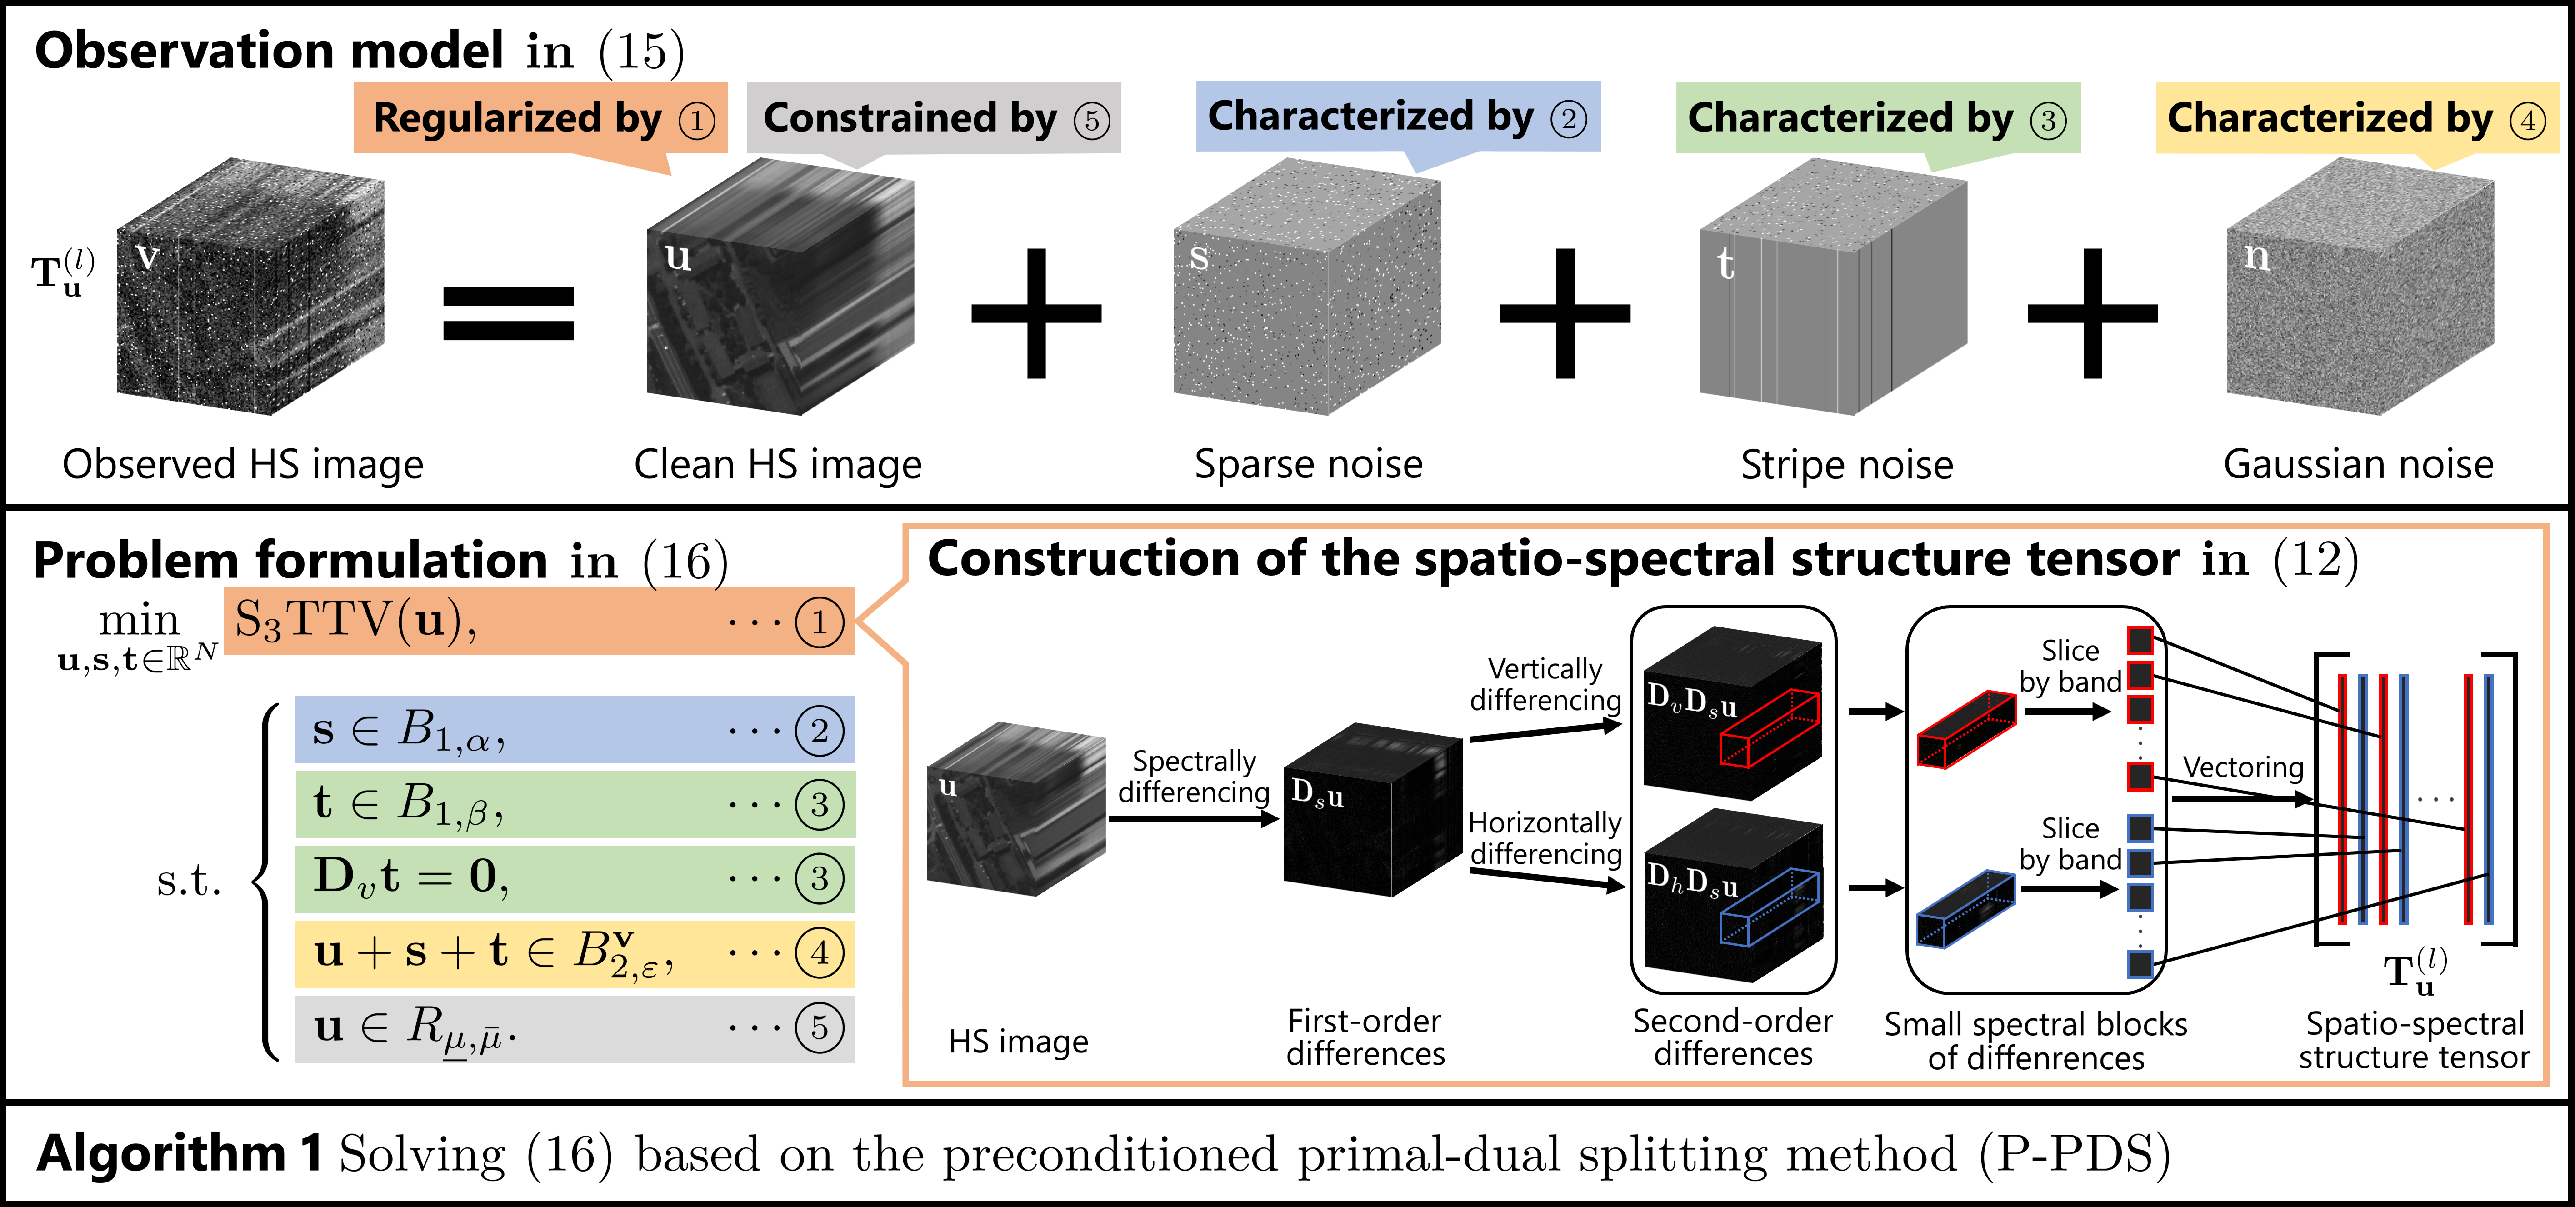
\includegraphics[width=\hsize]{./fig_supplement/Illustration_proposed_method.pdf}
	\end{center}
	\caption{Illustration of the proposed method, i.e., $\SSSTTV$.}
	\vspace{-2mm}
	\label{fig:schematic_diagram}
\end{figure*}

In the following, we first describe the design of the $\SSSTTV$ regularization function.
Next, we consider a situation where an HS image is contaminated with mixed noise and introduce the corresponding observation model.
Based on this model, we formulate an HS image denoising problem as a constrained convex optimization problem involving the $\SSSTTV$ regularization function.
% Based on this model, we formulate an HS image denoising problem as a constrained convex optimization problem . 
Finally, we derive an algorithm based on P-PDS to efficiently solve the optimization problem.
A schematic diagram of $\SSSTTV$ is shown in Fig.~\ref{fig:schematic_diagram}.

\subsection{Spatio-Spectral Structure Tensor Total Variation ($\SSSTTV$)}
\label{subsec:S3TTV}
%% S3TTV-1 ver2 20231116 1行目のSSSTのあと一言でLuの性質をまとめるのは不可能だから、いったんこれはおいといて、あとで1文使って補足する
Before describing the proposed regularization function, we introduce the notion of \textit{spatio-spectral structure tensor}\footnote{In the SSST paper~\cite{Kurihara2017SSST}, a structure tensor with the same name as the one we proposed (i.e., spatio-spectral structure tensor) is introduced. However, they are essentially different because the structure tensor in SSST consists of first-order differences, whereas that in our regularization function consists of second-order spatio-spectral differences.}.
First, for a given HS image $\HSIClean$, we calculate the second-order spatial-spectral differences $\DiffOpv \DiffOps \HSIClean$ and $\DiffOph \DiffOps \HSIClean$.
Next, we extract \textit{small spectral blocks} by cropping the second-order spatio-spectral differences to the size $\NumBlockVertical \times \NumBlockHorizontal (\NumBlockVertical << \NumVertical, \NumBlockHorizontal << \NumHorizontal)$ for all bands\footnote{At the boundaries, the block cannot be cropped to an $\NumBlockVertical \times \NumBlockHorizontal \times \NumBand$ size. For example, when the difference is cropped to a $3 \times 3 \times \NumBand$ block at a center $(1, 1)$, a $2 \times 2 \times \NumBand$ block is created. In this case, we pad the lacking areas with pixels on the opposite boundaries to make the block $\NumBlockVertical \times \NumBlockHorizontal \times \NumBand$.}.
% Next, we divide the second-order spatio-spectral differences into the \textit{small spectral blocks} that are rectangular with $\NumBlockVertical (\NumBlockVertical << \NumVertical)$ vertical pixels and $\NumBlockHorizontal (\NumBlockHorizontal << \NumHorizontal)$ horizontal pixels in the spatial domain and contain all $\NumBand$ bands\footnote{When extracting small spectral blocks at the boundaries of the second-order spatio-spectral difference cube, we treat the cube as if it were repeated vertically and horizontally. For example, the pixels outside on the right are interpolated by those on the left.}.
% The vectorized second-order spatio-spectral differences of $\IndexBand$-band in the $\IndexBlock$-th small spectral block are denoted by $\lbrack \DiffOpv \DiffOps \HSIClean \rbrack_{\IndexBand}^{(\IndexBlock)} \in \RealSpace{\NumBlockVertical \NumBlockHorizontal}$ and $\lbrack \DiffOph \DiffOps \HSIClean \rbrack_{\IndexBand}^{(\IndexBlock)} \in \RealSpace{\NumBlockVertical \NumBlockHorizontal}$.
Then, the $\IndexBlock$-th spatio-spectral structure tensor $\SmallBlock{\IndexBlock}$ is defined by vectorizing the second-order spatio-spectral differences in the $\IndexBlock$-th small spectral block by band and arranging them in parallel as follows:
\begin{equation}
\begin{split}
    \label{eq:SSST}
    \SmallBlock{\IndexBlock} :=  
    &\bigl( \lbrack \DiffOpv \DiffOps \HSIClean \rbrack_{1}^{(\IndexBlock)} \: 
    \lbrack\DiffOph \DiffOps \HSIClean \rbrack_{1}^{(\IndexBlock)} \\ 
    & \quad \cdots \lbrack \DiffOpv \DiffOps \HSIClean \rbrack_{\NumBand}^{(\IndexBlock)} \:
    \lbrack\DiffOph \DiffOps \HSIClean \rbrack_{\NumBand}^{(\IndexBlock)} 
    \bigr) \in \RealSpace{\NumBlockVertical \NumBlockHorizontal \times 2\NumBand}.
\end{split}
\end{equation}
where $\lbrack \DiffOpv \DiffOps \HSIClean \rbrack_{\IndexBand}^{(\IndexBlock)} \in \RealSpace{\NumBlockVertical \NumBlockHorizontal}$ and $\lbrack \DiffOph \DiffOps \HSIClean \rbrack_{\IndexBand}^{(\IndexBlock)} \in \RealSpace{\NumBlockVertical \NumBlockHorizontal}$ are the second-order spatio-spectral differences of $\IndexBand$-th band in the $\IndexBlock$-th small spectral block.
% where $\NumBlockVertical$ and $\NumBlockHorizontal$ are the number of vertical and horizontal pixels in a band of a small spectral block, respectively, and $\lbrack \DiffOpv \DiffOps \HSIClean \rbrack_{\IndexBand}^{(\IndexBlock)} \in \RealSpace{\NumBlockVertical \NumBlockHorizontal}$ and $\lbrack \DiffOph \DiffOps \HSIClean \rbrack_{\IndexBand}^{(\IndexBlock)} \in \RealSpace{\NumBlockVertical \NumBlockHorizontal}$ are the spatio-spectral difference vectors in the $\IndexBlock$-th small spectral block of $\IndexBand$-th band.
Since HS images have the strong correlation across all bands, $\lbrack \DiffOpv \DiffOps \HSIClean \rbrack_{1}^{(\IndexBlock)}, \ldots, \lbrack \DiffOpv \DiffOps \HSIClean \rbrack_{\NumBand}^{(\IndexBlock)}$ and $\lbrack \DiffOph \DiffOps \HSIClean \rbrack_{1}^{(\IndexBlock)}, \ldots, \lbrack \DiffOph \DiffOps \HSIClean \rbrack_{\NumBand}^{(\IndexBlock)}$ are similar vectors, respectively, i.e., the columns of $\SmallBlock{\IndexBlock}$ are approximately linearly dependent.
% For small spectral blocks around image boundaries, we use periodic boundary expansion.
The flow of constructing the spatio-spectral structure tensor is depicted in the middle right of Fig.~\ref{fig:schematic_diagram}.

%% S3TTV-1 ver1
% Before describing the proposed regularization function, we introduce \textit{spatio-spectral structure tensor}\footnote{In the SSST paper~\cite{Kurihara2017SSST}, a structure tensor with the same name as the one we proposed (i.e., spatio-spectral structure tensor) is introduced. However, they are essentially different because the structure tensor in SSST consists of first-order differences, whereas that in our regularization consists of second-order spatio-spectral differences.}, which is a matrix in a norm of the function.
% % Before describing the proposed regularization function, we introduce \textit{spatio-spectral structure tensor}\footnote{In the SSST paper~\cite{Kurihara2017SSST}, a structure tensor with the same name as the one we proposed (i.e., spatio-spectral structure tensor) is introduced. However, they are essentially different because the structure tensor in SSST consists of first-order differences, whereas that in our regularization consists of second-order spatio-spectral differences.}, which is a matrix to model the correlation of second-order differences.
% First, we calculate the spatial-spectral second-order differences $\DiffOpv \DiffOps \HSIClean$ and $\DiffOph \DiffOps \HSIClean$ for an HS image $\HSIClean$.
% % First, we calculate the spatial-spectral second-order differences of an HS image $\HSIClean$, $\DiffOpv \DiffOps \HSIClean$ and $\DiffOph \DiffOps \HSIClean$.
% Next, we divide the second-order spatio-spectral differences into 3D small blocks which are rectangular in the spatial domain and contain all bands.
% % Next, we divide the second-order spatio-spectral differences into 3D small blocks as shown in Fig.~\ref{fig:Construction_structure_tensor}.
% % The shape of each small block is rectangle in the spatial domain and contains all bands.
% Then, the $\IndexBlock$-th spatio-spectral structure tensor for $\HSIClean$ is defined by
% \begin{equation}
% \begin{split}
%     \label{eq:SSST}
%     \SmallBlock{\IndexBlock} :=  
%     &\bigl( \lbrack \DiffOpv \DiffOps \HSIClean \rbrack_{1}^{(\IndexBlock)} \: 
%     \lbrack\DiffOph \DiffOps \HSIClean \rbrack_{1}^{(\IndexBlock)} \\ 
%     & \quad \cdots \lbrack \DiffOpv \DiffOps \HSIClean \rbrack_{\NumBand}^{(\IndexBlock)} \:
%     \lbrack\DiffOph \DiffOps \HSIClean \rbrack_{\NumBand}^{(\IndexBlock)} 
%     \bigr) \in \RealSpace{\NumBlockVertical \NumBlockHorizontal \times 2\NumBand},
% \end{split}
% \end{equation}
% where $\NumBlockVertical$ and $\NumBlockHorizontal$ are the number of vertical and horizontal pixels in a one band of a small block, respectively, and $\lbrack \DiffOpv \DiffOps \HSIClean \rbrack_{\IndexBand}^{(\IndexBlock)} \in \RealSpace{\NumBlockVertical \NumBlockHorizontal}$ and $\lbrack \DiffOph \DiffOps \HSIClean \rbrack_{\IndexBand}^{(\IndexBlock)} \in \RealSpace{\NumBlockVertical \NumBlockHorizontal}$ are the $\IndexBand$-th band in the $\IndexBlock$-th small block.
% To handle small blocks around image boundaries, we use periodic boundary expansion.
% The flow of constructing the spatio-spectral structure tensor is depicted in Fig.~\ref{fig:Construction_structure_tensor}.

To capture the spatial piecewise-smoothness, the spatial similarity between adjacent bands, and the spectral correlation of an HS image, we propose a regularization function using the spatio-spectral structure tensors as follows:
\begin{equation}
    \label{eq:S3TTV_Lu}
    \textstyle \SSSTTV (\HSIClean) := \sum_{\IndexBlock=1}^{\NumBlock} \| \SmallBlock{\IndexBlock} \|_{*},
\end{equation}
where $\NumBlock$ is the number of the extracted small spectral blocks.
We call this function as \textit{Spatio-Spectral Structure Tensor Total Variation} ($\SSSTTV$).
Here, $\SmallBlock{\IndexBlock}$ is represented with an operator $\ExpantionOp{\IndexBlock} \in \RealSpace{2 \NumBlockVertical \NumBlockHorizontal \NumBand \times 2 \NumVertical \NumHorizontal \NumBand}$ that extracts the $\IndexBlock$-th small spectral block as
\begin{equation}
    \label{eq:rewrite_Lu}
    \SmallBlock{\IndexBlock}
    = \ExpantionOp{\IndexBlock} \DiffOpSp \DiffOps \HSIClean.
\end{equation}

Rather than directly suppressing some norm of the spatial differences, $\SSSTTV$ suppresses that of the spatial differences of the spectral differences (i.e., the second-order spatio-spectral differences), which preserves spatial similarity between adjacent bands.
% $\SSSTTV$ does not directly suppress some norm of spatial differences, but suppresses that of spatial differences of spectral differences (i.e., second-order spatio-spectral differences), similar to SSTV. 
% Therefore, $\SSSTTV$ can remove noise while preserving the consistency of the spatial structure between adjacent bands.
% Therefore, $\SSSTTV$ can remove noise while maintaining the consistency of spatial components between adjacent bands.
In addition, since the second-order difference vectors of each band are horizontally aligned in the structure tensors, $\SSSTTV$ can capture strong correlation across all bands when the sum of singular values of $\SmallBlock{\IndexBlock}$ is reduced.
This is because the stronger the correlation across all bands in HS images is, the more approximately linearly dependent the columns of $\SmallBlock{\IndexBlock}$ are.
% This is because strong correlation across all bands in HS image makes the columns of $\SmallBlock{\IndexBlock}$ approximately linearly dependent.


\subsection{HS Image Denoising Problem by $\SSSTTV$}
\label{subsec:HSI_Denoising_Problem}
An observed HS image $\HSIObsv \in \RealSpace{\NumElement}$ contaminated by mixed noise is modeled by
\begin{equation}
    \label{eq:Obsevation_model}
    \HSIObsv = \bar{\HSIClean} + \bar{\NoiseSparse} + \bar{\NoiseStripe} + \NoiseGauss,
\end{equation}
where $\bar{\HSIClean}$ is a clean HS image, $\bar{\NoiseSparse}$ is sparse noise, $\bar{\NoiseStripe}$ is stripe noise, and $\NoiseGauss$ is Gaussian noise, respectively.
% where $\bar{\HSIClean}$ is a clean HS image, $\bar{\NoiseSparse}$ is a sparse noise that models outliers and missing data, $\bar{\NoiseStripe}$ is a stripe noise caused by , and $\NoiseGauss$ represent a clean HS image,  and a random noise, respectively.

Based on the above observation model, we formulate an HS image denoising problem involving $\SSSTTV$ as a constrained convex optimization problem with the following form:
\begin{equation}
    \label{prob:S3TTV_denoising}
    \min_{\HSIClean, \NoiseSparse, \NoiseStripe \in \RealSpace{\NumElement}} \SSSTTV(\HSIClean) \: \mathrm{s.t.} \:
    \begin{cases} 
        \NoiseSparse \in \BallSparse, \\ 
        \NoiseStripe \in \BallStripe, \\
        \DiffOpv \NoiseStripe = \mathbf{0}, \\
        \HSIClean + \NoiseSparse + \NoiseStripe \in \BallFidel, \\  
        \HSIClean \in \SetRange,
    \end{cases}
\end{equation}
where
\begin{align}
    \label{eq:constraint_sparse}
    &\BallSparse := \{ \VarOne \in \RealSpace{\NumElement} | \:
    \|\VarOne\|_{1} \leq \RadiusSparse \},  \\
    \label{eq:constraint_stripe}
    &\BallStripe := \{ \VarOne \in \RealSpace{\NumElement} | \:
    \|\VarOne\|_{1} \leq \RadiusStripe \},  \\
    \label{eq:constraint_fidel}
    &\BallFidel := \{ \VarOne \in \RealSpace{\NumElement} | \:
    \|\VarOne - \HSIObsv\|_2 \leq \RadiusFidel \},  \\
    \label{eq:constraint_box}
    &\SetRange := \{ \VarOne \in \RealSpace{\NumElement} | \:
    \MinRange \leq \ElementOne{\IndexOne} \leq \MaxRange  \: (\IndexOne = 1,\dots , \NumElement) \}.
\end{align}
% and $\SetZero$ denotes the (closed convex) set only containing the zero vector.

The first constraint characterizes sparse noise $\NoiseSparse$ with the zero-centered $\ell_1$-ball of the radius $\RadiusSparse > 0$.
The second constraint controls the intensity of stripe noise $\NoiseStripe$ and the third constraint captures the vertical flatness property by imposing zero to the vertical gradient of $\NoiseStripe$.
These constraints effectively characterize stripe noise~\cite{Naganuma2022Destriping}.
The fourth constraint serves as data-fidelity with the $\HSIObsv$-centered $\ell_2$-ball of the radius $\RadiusFidel > 0$.
% The third and fourth constraints model the sparsity and flatness of the (vertical) stripe noise.
% However, unlike the original paper, we use constraint that controls the intensity of stripe noise $\NoiseStripe$ instead of adding it to the objective function.
% This is because $\RadiusStripe$ can be determined based solely on the intensity of stripe noise (independent of the other terms in the objective function), making it much easier to adjust the hyperparameters.
% For the same reason, we employ data fidelity constraint and the constraint characterizing sparse noise, as addressed, for example, in~\cite{Constraint_Afonso2011,Constraint_Chierchia2015, Constraint_Ono2015, Constraint_Ono2017, Constraint_Ono2019}.
% Because $\RadiusFidel$ and $\RadiusSparse$ can be determined based solely on the intensity of each noise (independently of the other terms in the objective function), such a data fidelity constraint makes the adjustment of the hyperparameters much easier than when a data fidelity term is added to the objective function. 
% These advantages are also addressed, for example, in~\cite{Constraint_Afonso2011,Constraint_Chierchia2015, Constraint_Ono2015, Constraint_Ono2017, Constraint_Ono2019}.
The fifth constraint is a box constraint with $\MinRange < \MaxRange$ which represents the dynamic range of $\HSIClean$.
For normalized HS images, we can set $\MinRange = 0$ and $\MaxRange = 1$.


Using the first, second, and fourth constraints instead of adding terms to the objective function makes it much easier to adjust the parameters $\RadiusSparse$, $\RadiusStripe$, and $\RadiusFidel$.
% Using the first, second, and third constraints instead of adding terms to the objective function makes it easier to adjust the parameters $\RadiusFidel$, $\RadiusSparse$, and $\RadiusStripe$~\cite{Constraint_Afonso2011,Constraint_Chierchia2015, Constraint_Ono2015, Constraint_Ono2017, Constraint_Ono2019}.
This is because by expressing multiple terms as constraints, rather than adding them to the objective function, the hyperparameters associated with each term are converted to be independent of each other, and appropriate parameters can be determined without interdependence.
% This is because these constraints are decoupled and the appropriate parameters can be determined independently.
Such advantage has been addressed, e.g., in~\cite{Constraint_Afonso2011,Constraint_Chierchia2015, Constraint_Ono2015, Constraint_Ono2017, Constraint_Ono2019}.
\begin{figure}[!t]
	\begin{algorithm}[H]
	    \caption{P-PDS-based solver for (18)}
	   % \caption{The DP-PDS algorithm for \eqref{prob:denoising2PPDS}}
		\label{algo_DPPDS}
		\begin{algorithmic}[1]
			% \renewcommand{\algorithmicrequire}{\textbf{Input:}}
			% \renewcommand{\algorithmicensure}{\textbf{Output:}}
			\REQUIRE $\HSIClean^{(0)}, \NoiseSparse^{(0)}, \NoiseStripe^{(0)},  \VarDualMatrix{1,\IndexBlock}^{(0)}(\IndexBlock = 1, \ldots \NumBlock), \VarDual{2}^{(0)}, \VarDual{3}^{(0)}$
			\ENSURE $\HSIClean^{(\IndexAlg)}$
			\WHILE {A stopping criterion is not satisfied}
    			\STATE $\HSIClean^{(\IndexAlg+1)} \leftarrow$ \\ $ \qquad  \Projection{\SetRange}\left( \HSIClean^{(\IndexAlg)} - \ParamStepsize{\HSIClean}  \bigl(\sum_{\IndexBlock=1}^{\NumBlock} \DiffOpBandT \DiffOpSpT \ExpantionOp{\IndexBlock}^{\top} \VarDualMatrix{1,\IndexBlock}^{(\IndexAlg)} + \VarDual{3}^{(\IndexAlg)} \bigr) \right)$;
    			\STATE $\NoiseSparse^{(\IndexAlg+1)} \leftarrow \prox_{\ParamStepsize{\NoiseSparse}, \FuncIndicator{\BallSparse}} \left( \NoiseSparse^{(\IndexAlg)} - \ParamStepsize{\NoiseSparse} \VarDual{3}^{(\IndexAlg)} \right)$;
                    \STATE $\NoiseStripe^{(\IndexAlg+1)} \leftarrow \prox_{\ParamStepsize{\NoiseStripe}, \FuncIndicator{\BallStripe}} \left( \NoiseStripe^{(\IndexAlg)} - \ParamStepsize{\NoiseStripe} \bigl( \DiffOpVertT \VarDual{2}^{(\IndexAlg)} + \VarDual{3}^{(\IndexAlg)} \bigr) \right)$;
                    \STATE $\ResHSIClean \leftarrow 2\HSIClean^{(\IndexAlg+1)} - \HSIClean^{(\IndexAlg)}$;
                    \STATE $\ResNoiseSparse \leftarrow 2\NoiseSparse^{(\IndexAlg+1)} - \NoiseSparse^{(\IndexAlg)}$;
                    \STATE $\ResNoiseStripe \leftarrow 2\NoiseStripe^{(\IndexAlg+1)} - \NoiseStripe^{(\IndexAlg)}$;
    			\FOR{$\IndexBlock = 1, \ldots, \NumBlock$}
    			    \STATE $\VarDualMatrix{1,\IndexBlock}^{'} \leftarrow \VarDualMatrix{1,\IndexBlock}^{(\IndexAlg)} + \ParamStepsize{\VarDualMatrix{1, \IndexBlock}} \ExpantionOp{\IndexBlock} \DiffOpSp \DiffOpBand \ResHSIClean$;
    			    \STATE $\VarDualMatrix{1,\IndexBlock}^{(\IndexAlg+1)} \leftarrow \VarDualMatrix{1,\IndexBlock}^{'} - \ParamStepsize{\VarDualMatrix{1, \IndexBlock}} \prox_{\ParamStepsize{\VarDualMatrix{1, \IndexBlock}}^{-1}, \| \cdot \|_{*}} \left(\ParamStepsize{\VarDualMatrix{1, \IndexBlock}}^{-1} \VarDualMatrix{1,\IndexBlock}^{'}\right) $;
    		    \ENDFOR
                    \STATE $\VarDual{2}^{(\IndexAlg+1)} \leftarrow \VarDual{2}^{(\IndexAlg)} + \ParamStepsize{\VarDual{2}} \DiffOpVert \ResNoiseStripe$;
    			\STATE $\VarDual{3}^{'} \leftarrow \VarDual{3}^{(\IndexAlg)} + \ParamStepsize{\VarDual{3}} \left( \ResHSIClean + \ResNoiseSparse + \ResNoiseStripe \right)$;
    			\STATE $\VarDual{3}^{(\IndexAlg+1)} \leftarrow \VarDual{3}^{'} - \ParamStepsize{\VarDual{3}} \Projection{\BallFidel} \left(\ParamStepsize{\VarDual{3}}^{-1} \VarDual{3}^{'}  \right)$;
        % 		\STATE $\VarDual{2}^{(\IndexAlg+1)} \leftarrow \VarDual{2}^{'} - \ParamStepsize{\VarDual{2}} \prox_{\frac{1}{\ParamStepsize{\VarDual{2}}} \iota_{\BallFidel}} \left(\frac{1}{\ParamStepsize{\VarDual{2}}} \VarDual{2}^{'}  \right)$;
    			\STATE $\IndexAlg \leftarrow \IndexAlg + 1$;
			\ENDWHILE
		\end{algorithmic}
	\end{algorithm}
	\vspace{-2mm}
\end{figure}


\subsection{Optimization}
\label{subsec:Optim}
We develop an efficient solver for Prob.~\eqref{prob:S3TTV_denoising} based on P-PDS~\cite{Pock2011PPDS}.
Using the indicator functions $\FuncIndicator{\SetZero}$, $\FuncIndicator{\BallFidel}$, $\FuncIndicator{\BallStripe}$, $\FuncIndicator{\BallSparse}$, and $\FuncIndicator{\SetRange}$, we rewrite Prob.~\eqref{prob:S3TTV_denoising} into an equivalent form:
\begin{align}
    \label{prob:denoising2PPDS}
    \min_{
    \substack{
        \HSIClean, \NoiseSparse, \NoiseStripe\\ 
        \VarDual{1,1}, \ldots , \VarDual{1,\NumBlock}, 
        \VarDual{2}, \VarDual{3}}} \:
    & \sum_{\IndexBlock=1}^{\NumBlock} \| 
    \VarDual{1, \IndexBlock} \|_{*}
    + \FuncIndicator{\SetZero} (\VarDual{2})
    + \FuncIndicator{\BallFidel} (\VarDual{3}) \nonumber \\
    & + \FuncIndicator{\BallSparse} (\NoiseSparse) 
    + \FuncIndicator{\BallStripe} (\NoiseStripe)
    + \FuncIndicator{\SetRange} (\HSIClean),  \nonumber \\
    & \mathrm{s.t.} \:
    \begin{cases} 
    \VarDual{1,1} = \ExpantionOp{1} \DiffOpSp \DiffOps \HSIClean, \\ 
    \vdots \\ 
    \VarDual{1,\NumBlock} = \ExpantionOp{\NumBlock} \DiffOpSp \DiffOps \HSIClean, \\ 
    \VarDual{2} = \DiffOpv \NoiseStripe, \\
    \VarDual{3} = \HSIClean + \NoiseSparse + \NoiseStripe. 
    \end{cases}
\end{align}
% \begin{align}
%     \label{prob:denoising2PPDS}
%     \min_{
%     \substack{
%         \HSIClean, \NoiseSparse, 
%         \VarDual{1}, \\ 
%         \VarDual{2,1}, \ldots , \VarDual{1,\NumBlock}}} \:
%     & \FuncIndicator{\BallFidel} (\VarDual{2}) 
%     + \sum_{\IndexBlock=1}^{\NumBlock} \| \VarDual{2, \IndexBlock} \|_{*}
%     + \FuncIndicator{\BallSparse} (\NoiseSparse) 
%     + \FuncIndicator{\SetRange} (\HSIClean)  \nonumber \\
%     \mathrm{s.t.} \: & 
%     \begin{cases} 
%     \VarDual{1,1} = \ExpantionOp{1} \DiffOpSp \DiffOps \HSIClean, \\ 
%     \vdots \\ 
%     \VarDual{1,\NumBlock} = \ExpantionOp{\NumBlock} \DiffOpSp \DiffOps \HSIClean, \\ 
%     \VarDual{2} = \HSIClean + \NoiseSparse, 
%     \end{cases}
% \end{align}
Then, by defining,
\begin{align}
    \label{eq:FuncMapping}
    & \FuncPrimal{1} (\HSIClean) := \FuncIndicator{\SetRange} (\HSIClean), \nonumber \\
    & \FuncPrimal{2} (\NoiseSparse) := \FuncIndicator{\BallSparse} (\NoiseSparse), \nonumber \\
    & \FuncPrimal{3} (\NoiseStripe) := \FuncIndicator{\BallStripe} (\NoiseStripe), \nonumber \\
    & \FuncDual{1} (\VarDual{1, 1}) := \| \VarDual{1, 1} \|_{*}, \ldots, \FuncDual{\NumBlock}(\VarDual{1, \NumBlock}) := \| \VarDual{1, \NumBlock} \|_{*}, \nonumber \\
    & \FuncDual{\NumBlock + 1} (\VarDual{2}) := \FuncIndicator{\SetZero} (\VarDual{2}), \nonumber \\
    & \FuncDual{\NumBlock + 2} (\VarDual{3}) := \FuncIndicator{\BallFidel} (\VarDual{3}),
\end{align}
Prob.~\eqref{prob:denoising2PPDS} is reduced to Prob.~\eqref{prob:convex_optim_prob}.
% Let $\HSIClean$, $\NoiseSparse$, and $\NoiseStripe$ be the primal variables and $\VarDual{1,1}, \ldots , \VarDual{1,\NumBlock}, \VarDual{2}, \VarDual{3}$ be the dual variables in Prob.~\eqref{prob:convex_optim_prob}, then Prob.~\eqref{prob:denoising2PPDS} are equivalent forms to Prob.~\eqref{prob:convex_optim_prob}.
Therefore, P-PDS is applicable to Prob.~\eqref{prob:denoising2PPDS}.
% \begin{figure}[!t]
	\begin{algorithm}[H]
	    \caption{P-PDS-based solver for (18)}
	   % \caption{The DP-PDS algorithm for \eqref{prob:denoising2PPDS}}
		\label{algo_DPPDS}
		\begin{algorithmic}[1]
			% \renewcommand{\algorithmicrequire}{\textbf{Input:}}
			% \renewcommand{\algorithmicensure}{\textbf{Output:}}
			\REQUIRE $\HSIClean^{(0)}, \NoiseSparse^{(0)}, \NoiseStripe^{(0)},  \VarDualMatrix{1,\IndexBlock}^{(0)}(\IndexBlock = 1, \ldots \NumBlock), \VarDual{2}^{(0)}, \VarDual{3}^{(0)}$
			\ENSURE $\HSIClean^{(\IndexAlg)}$
			\WHILE {A stopping criterion is not satisfied}
    			\STATE $\HSIClean^{(\IndexAlg+1)} \leftarrow$ \\ $ \qquad  \Projection{\SetRange}\left( \HSIClean^{(\IndexAlg)} - \ParamStepsize{\HSIClean}  \bigl(\sum_{\IndexBlock=1}^{\NumBlock} \DiffOpBandT \DiffOpSpT \ExpantionOp{\IndexBlock}^{\top} \VarDualMatrix{1,\IndexBlock}^{(\IndexAlg)} + \VarDual{3}^{(\IndexAlg)} \bigr) \right)$;
    			\STATE $\NoiseSparse^{(\IndexAlg+1)} \leftarrow \prox_{\ParamStepsize{\NoiseSparse}, \FuncIndicator{\BallSparse}} \left( \NoiseSparse^{(\IndexAlg)} - \ParamStepsize{\NoiseSparse} \VarDual{3}^{(\IndexAlg)} \right)$;
                    \STATE $\NoiseStripe^{(\IndexAlg+1)} \leftarrow \prox_{\ParamStepsize{\NoiseStripe}, \FuncIndicator{\BallStripe}} \left( \NoiseStripe^{(\IndexAlg)} - \ParamStepsize{\NoiseStripe} \bigl( \DiffOpVertT \VarDual{2}^{(\IndexAlg)} + \VarDual{3}^{(\IndexAlg)} \bigr) \right)$;
                    \STATE $\ResHSIClean \leftarrow 2\HSIClean^{(\IndexAlg+1)} - \HSIClean^{(\IndexAlg)}$;
                    \STATE $\ResNoiseSparse \leftarrow 2\NoiseSparse^{(\IndexAlg+1)} - \NoiseSparse^{(\IndexAlg)}$;
                    \STATE $\ResNoiseStripe \leftarrow 2\NoiseStripe^{(\IndexAlg+1)} - \NoiseStripe^{(\IndexAlg)}$;
    			\FOR{$\IndexBlock = 1, \ldots, \NumBlock$}
    			    \STATE $\VarDualMatrix{1,\IndexBlock}^{'} \leftarrow \VarDualMatrix{1,\IndexBlock}^{(\IndexAlg)} + \ParamStepsize{\VarDualMatrix{1, \IndexBlock}} \ExpantionOp{\IndexBlock} \DiffOpSp \DiffOpBand \ResHSIClean$;
    			    \STATE $\VarDualMatrix{1,\IndexBlock}^{(\IndexAlg+1)} \leftarrow \VarDualMatrix{1,\IndexBlock}^{'} - \ParamStepsize{\VarDualMatrix{1, \IndexBlock}} \prox_{\ParamStepsize{\VarDualMatrix{1, \IndexBlock}}^{-1}, \| \cdot \|_{*}} \left(\ParamStepsize{\VarDualMatrix{1, \IndexBlock}}^{-1} \VarDualMatrix{1,\IndexBlock}^{'}\right) $;
    		    \ENDFOR
                    \STATE $\VarDual{2}^{(\IndexAlg+1)} \leftarrow \VarDual{2}^{(\IndexAlg)} + \ParamStepsize{\VarDual{2}} \DiffOpVert \ResNoiseStripe$;
    			\STATE $\VarDual{3}^{'} \leftarrow \VarDual{3}^{(\IndexAlg)} + \ParamStepsize{\VarDual{3}} \left( \ResHSIClean + \ResNoiseSparse + \ResNoiseStripe \right)$;
    			\STATE $\VarDual{3}^{(\IndexAlg+1)} \leftarrow \VarDual{3}^{'} - \ParamStepsize{\VarDual{3}} \Projection{\BallFidel} \left(\ParamStepsize{\VarDual{3}}^{-1} \VarDual{3}^{'}  \right)$;
        % 		\STATE $\VarDual{2}^{(\IndexAlg+1)} \leftarrow \VarDual{2}^{'} - \ParamStepsize{\VarDual{2}} \prox_{\frac{1}{\ParamStepsize{\VarDual{2}}} \iota_{\BallFidel}} \left(\frac{1}{\ParamStepsize{\VarDual{2}}} \VarDual{2}^{'}  \right)$;
    			\STATE $\IndexAlg \leftarrow \IndexAlg + 1$;
			\ENDWHILE
		\end{algorithmic}
	\end{algorithm}
	\vspace{-2mm}
\end{figure}
%\begin{table*}[t]
%    \begin{center}
%        \caption{MPSNRs of the Simulated HS Image Denoising Results.}
%        \label{tab:MPSNR}
%            \scalebox{0.85}{
%        \begin{tabular}{cc ccccccccc}
%            \toprule
%                Image & Noise & SSTV~\cite{Aggarwal2016SSTV} & HSSTV1~\cite{Takeyama2020HSSTV} & HSSTV2~\cite{Takeyama2020HSSTV} & $\llHTV$~\cite{Wang2021l0l1HTV} & STV~\cite{Lefkimmiatis2015STV} & SSST~\cite{Kurihara2017SSST} & LRTDTV~\cite{Wang2018LRTDTV} & TPTV~\cite{Chen2023TPTV} & $\SSSTTV$ \\
%            \cmidrule(lr){1-11}
%            % \vspace{-0.5mm}
%                \multirow{6}{*}{Jasper Ridge} & Case 1 & 
%                39.32 & 38.98 & 38.92 & 38.47 & 29.81 & 36.56 & 37.85 & \textbf{40.29} & \underline{39.82}\\
%                & Case 2 & 
%                34.24 & 34.01 & 34.67 & 34.00 & 27.23 & 32.07 & 34.87 & \underline{35.79} & \textbf{36.00} \\
%                & Case 3 & 
%                39.07 & \underline{39.29} & 38.31 & 38.92 & 30.72 & 37.63 & 35.99 & 38.14 & \textbf{40.10} \\
%                & Case 4 & 
%                34.21 & 34.81 & 33.90 & 34.68 & 28.08 & 34.88 & 33.69 & \underline{35.51} & \textbf{35.72} \\
%                & Case 5 & 
%                39.30 & 39.06 & 38.55 & 38.35 & 29.54 & 35.67 & 36.05 & \underline{39.24} & \textbf{39.65} \\
%                & Case 6 & 
%                34.59 & 34.22 & 34.99 & 34.15 & 26.95 & 30.95 & 33.64 & \underline{35.23} & \textbf{35.89} \\
%
%            \cmidrule(lr){1-11}
%            
%            \multirow{6}{*}{Pavia University} & Case 1 & 
%            	38.43 & 38.34 & 38.23 & 37.88 & 29.84 & 35.16 & 35.08 & \underline{38.74} & \textbf{39.24} \\
%                & Case 2 & 
%                32.87 & 33.38 & 33.07 & 32.67 & 27.49 & 31.63 & 32.53 & \textbf{34.12} & \underline{33.94}  \\
%                & Case 3 & 
%                39.34 & \underline{39.43} & 38.43 & 39.04 & 30.74 & 36.52 & 32.34 & 38.14 & \textbf{39.80}  \\
%                & Case 4 & 
%                34.26 &\underline{34.88} & 33.82 & 34.75 & 28.33 & 34.69 & 30.82 & 34.03 & \textbf{35.17} \\
%                & Case 5 & 
%                \underline{38.56} & 38.48 & 38.22 & 37.73 & 29.62 & 34.25 & 32.44 & 38.29 & \textbf{38.78} \\
%                & Case 6 & 
%                32.88 & 33.42 & 33.19 & 32.52 & 27.24 & 30.50 & 30.89 & \underline{33.67} & \textbf{33.88} \\
%	            
%            \bottomrule
%        \end{tabular}
%        		}
%    \end{center}
%    % \vspace{-3mm}
%\end{table*}


\begin{table*}[t]
	\begin{center}
		\caption{MPSNRs of the Simulated HS Image Denoising Results.}
		\label{tab:MPSNR}
		\scalebox{0.75}{
			\begin{tabular}{cc ccccccccccc}
				\toprule
				Image & Noise & SSTV~\cite{Aggarwal2016SSTV} & HSSTV1~\cite{Takeyama2020HSSTV} & HSSTV2~\cite{Takeyama2020HSSTV} & $\llHTV$~\cite{Wang2021l0l1HTV} & STV~\cite{Lefkimmiatis2015STV} & SSST~\cite{Kurihara2017SSST} & LRTDTV~\cite{Wang2018LRTDTV} & FGSLR~\cite{Chen2022FGSLR} & TPTV~\cite{Chen2023TPTV} & FastHyMix~\cite{Zhuang2023FastHyMix} & $\SSSTTV$ \\
				\cmidrule(lr){1-13}
				% \vspace{-0.5mm}
				\multirow{8}{*}{Jasper Ridge} 
				& Case 1 &
				36.16 & \underline{36.25} & 35.66 & 35.40 & 28.15 & 35.03 & 35.08 & 33.68 & 34.25 & \textbf{38.77} & 35.43 \\
				& Case 2 & 
				\underline{39.32} & 38.98 & 38.92 & 38.47 & 29.81 & 36.56 & 37.85 & 35.65 & 39.01 & 27.86 & \textbf{39.82} \\
				& Case 3 & 
				34.24 & 34.01 & 34.67 & 34.00 & 27.23 & 32.07 & \underline{34.87} & 33.44 & 33.68 & 25.53 & \textbf{36.00} \\
				& Case 4 &
				42.50 & 41.45 & \underline{44.46} & 42.95 & 39.09 & 41.31 & 37.07 & 41.65 & \textbf{51.34} & 34.93 & 43.95 \\
				& Case 5 & 
				39.03 & \underline{39.26} & 38.33 & 38.88 & 30.72 & 37.63 & 36.00 & 35.62 & 37.92 & 35.21 & \textbf{39.90} \\
				& Case 6 & 
				34.19 & 34.79 & 33.91 & 34.52 & 28.08 & \underline{34.88} & 33.70 & 33.43 & 33.44 & 34.30 & \textbf{35.41} \\
				& Case 7 & 
				\underline{39.30} & 39.06 & 38.55 & 38.35 & 29.54 & 35.67 & 36.09 & 35.46 & 37.91 & 37.29 & \textbf{39.65} \\
				& Case 8 & 
				34.59 & 34.22 & \underline{34.99} & 34.15 & 26.95 & 30.95 & 33.64 & 33.23 & 33.08 & 23.19 & \textbf{35.89} \\
				
				\cmidrule(lr){1-13}
				
				\multirow{8}{*}{Pavia University}
				& Case 1 &
				35.64 & \underline{36.05} & 34.98 & 35.08 & 28.33 & 34.85 & 32.67 & 32.52 & 31.41 & \textbf{37.53} & 35.37 \\
				& Case 2 & 
				38.43 & 38.34 & 38.23 & 37.88 & 29.84 & 35.16 & 35.08 & 35.33 & 36.80 & \underline{38.91} & \textbf{39.24} \\
				& Case 3 & 
				32.87 & 33.38 & 33.07 & 32.67 & 27.49 & 31.63 & 32.53 & 31.88 & 31.04 & \textbf{35.91} & \underline{33.94} \\
				& Case 4 &
				41.01 & 40.50 & \underline{43.96} & 41.81 & 39.28 & 40.43 & 32.22 & 40.07 & \textbf{48.14} & 34.24 & 42.62 \\
				& Case 5 & 
				39.32 & \underline{39.42} & 38.44 & 39.06 & 30.74 & 36.52 & 32.34 & 35.41 & 35.75 & 34.70 & \textbf{39.78} \\
				& Case 6 & 
				34.24 & \underline{34.87} & 33.82 & 34.65 & 28.33 & 34.69 & 30.87 & 31.84 & 31.56 & 33.57 & \textbf{35.17} \\
				& Case 7 & 
				\underline{38.56} & 38.48 & 38.22 & 37.73 & 29.62 & 34.25 & 32.43 & 35.12 & 35.72 & 32.02 & \textbf{38.78} \\
				& Case 8 & 
				32.88 & \underline{33.42} & 33.19 & 32.52 & 27.24 & 30.50 & 30.88 & 31.65 & 31.06 & 31.77 & \textbf{33.88} \\
				
				\cmidrule(lr){1-13}
				
				\multirow{8}{*}{Beltsville}
				& Case 1 &
				35.20 & \underline{35.90} & 34.87 & 34.70 & 29.11 & 35.86 & 34.23 & 34.68 & 32.24 & \textbf{39.36} & 35.33 \\
				& Case 2 & 
				37.87 & 38.18 & 37.62 & 37.32 & 30.83 & 36.81 & \underline{38.71} & 36.73 & 37.82 & 37.86 & \textbf{39.40} \\
				& Case 3 & 
				32.95 & 33.94 & 32.93 & 32.76 & 28.39 & 32.39 & 34.18 & \underline{34.45} & 31.76 & \textbf{36.12} & 34.23 \\
				& Case 4 &
				41.16 & 40.84 & 41.37 & 41.45 & 37.96 & 40.21 & 38.69 & \underline{42.90} & \textbf{52.72} & 36.22 & 40.72 \\
				& Case 5 & 
				38.43 & \underline{38.73} & 37.99 & 38.11 & 30.73 & 37.04 & 33.47 & 36.64 & 36.68 & 35.11 & \textbf{39.65} \\
				& Case 6 & 
				33.91 & 34.64 & 33.72 & 34.20 & 28.62 & \underline{34.81} & 30.60 & 34.25 & 32.84 & 34.12 & \textbf{35.29} \\
				& Case 7 & 
				38.00 & \underline{38.21} & 37.62 & 37.21 & 30.05 & 35.43 & 32.97 & 36.45 & 36.99 & 37.18 & \textbf{38.85} \\
				& Case 8 & 
				33.14 & 33.98 & 33.25 & 32.72 & 27.84 & 30.97 & 30.59 & \underline{34.05} & 32.26 & 33.33 & \textbf{34.43} \\
				
				\bottomrule
			\end{tabular}
		}
	\end{center}
	% \vspace{-3mm}
\end{table*}
\begin{table*}[t]
    \begin{center}
        \caption{MSSIMs of the Simulated HS Image Denoising Results.}
        \label{tab:MSSIM}
        		\scalebox{0.75}{
        \begin{tabular}{cc ccccccccccc}
            \toprule
                Image & Noise & SSTV~\cite{Aggarwal2016SSTV} & HSSTV1~\cite{Takeyama2020HSSTV} & HSSTV2~\cite{Takeyama2020HSSTV} & $\llHTV$~\cite{Wang2021l0l1HTV} & STV~\cite{Lefkimmiatis2015STV} & SSST~\cite{Kurihara2017SSST} & LRTDTV~\cite{Wang2018LRTDTV} & FGSLR~\cite{Chen2022FGSLR} & TPTV~\cite{Chen2023TPTV} & FastHyMix~\cite{Zhuang2023FastHyMix} & $\SSSTTV$ \\
            \cmidrule(lr){1-13}
            % \vspace{-0.5mm}
				\multirow{8}{*}{Jasper Ridge}
				& Case 1 & 
				0.9218 & \underline{0.9367} & 0.9170 & 0.9013 & 0.7495 & 0.9318 & 0.9147 & 0.9175 & 0.8703 & \textbf{0.9659} & 0.9070 \\
				& Case 2 & 
                0.9588 & \textbf{0.9632} & 0.9552 & 0.9468 & 0.8227 & 0.9486 & 0.9542 & 0.9450 & 0.9504 & 0.8648 & \underline{0.9601} \\
                & Case 3 & 
                0.9026 & 0.9071 & 0.9082 & 0.8897 & 0.7165 & 0.8736 & 0.9122 & \underline{0.9144} & 0.8613 & 0.7726 & \textbf{0.9201} \\
                & Case 4 & 
                0.9782 & 0.9759 & 0.9774 & 0.9782 & 0.9739 & 0.9780 & 0.9572 & \underline{0.9830} & \textbf{0.9889} & 0.9090 & 0.9788 \\
                & Case 5 & 
                0.9539 & \textbf{0.9613} & 0.9481 & 0.9490 & 0.8428 & 0.9586 & 0.9319 & 0.9434 & 0.9363 & 0.9037 & \underline{0.9608} \\
                & Case 6 & 
                0.8808 & 0.9054 & 0.8775 & 0.8832 & 0.7446 & \textbf{0.9296} & 0.8794 & \underline{0.9108} & 0.8519 & 0.8888 & 0.9077 \\
                & Case 7 & 
                0.9585 & \textbf{0.9634} & 0.9518 & 0.9449 & 0.8144 & 0.9390 & 0.9328 & 0.9421 & 0.9416 & 0.9503 & \underline{0.9592} \\
                & Case 8 & 
                0.9071 & 0.9108 & \underline{0.9114} & 0.8895 & 0.7061 & 0.8439 & 0.8814 & 0.9086 & 0.8471 & 0.5912 & \textbf{0.9191} \\

            \cmidrule(lr){1-13}
            
            	\multirow{8}{*}{Pavia University}
            	& Case 1 &
            	0.9207 & \underline{0.9347} & 0.9067 & 0.9088 & 0.7170 & 0.9231 & 0.8600 & 0.9013 & 0.8074 & \textbf{0.9533} & 0.9119 \\
            	& Case 2 & 
            	0.9559 & \underline{0.9585} & 0.9478 & 0.9486 & 0.7889 & 0.9307 & 0.9166 & 0.9412 & 0.9307 & \textbf{0.9698} & 0.9582 \\
                & Case 3 & 
                0.8731 & 0.8882 & 0.8731 & 0.8672 & 0.6754 & 0.8533 & 0.8573 & 0.8829 & 0.8011 & \textbf{0.9445} & \underline{0.8928} \\
                & Case 4 & 
                0.9726 & 0.9716 & 0.9753 & 0.9730 & 0.9723 & 0.9727 & 0.9055 & \textbf{0.9793} & 0.9750 & 0.9310 & \underline{0.9754} \\
                & Case 5 & 
                0.9622 & \textbf{0.9657} & 0.9514 & 0.9584 & 0.8191 & 0.9435 & 0.8789 & 0.9421 & 0.9162 & 0.9163 & \underline{0.9625} \\
                & Case 6 & 
                0.8933 & \underline{0.9133} & 0.8830 & 0.8998 & 0.7180 & \textbf{0.9213} & 0.8148 & 0.8955 & 0.8166 & 0.8955 & 0.9089 \\
                & Case 7 & 
                \underline{0.9573} & \textbf{0.9598} & 0.9482 & 0.9473 & 0.7812 & 0.9160 & 0.8776 & 0.9390 & 0.9207 & 0.9122 & 0.9550 \\
                & Case 8 & 
                0.8736 & \underline{0.8892} & 0.8752 & 0.8640 & 0.6639 & 0.8152 & 0.8139 & 0.8790 & 0.8059 & 0.8712 & \textbf{0.8915} \\
                
            \cmidrule(lr){1-13}
            
	            \multirow{8}{*}{Beltsville}
	            & Case 1 & 
	            0.9099 & 0.9290 & 0.9035 & 0.8978 & 0.7282 & \underline{0.9327} & 0.8776 & 0.9134 & 0.8137 & \textbf{0.9642} & 0.9052 \\
	            & Case 2 &
	            0.9497 & 0.9550 & 0.9458 & 0.9425 & 0.8012 & 0.9410 & 0.9508 & 0.9482 & 0.9421 & \textbf{0.9663} & \underline{0.9605} \\
	            & Case 3 & 
	            0.8710 & 0.8931 & 0.8694 & 0.8696 & 0.6911 & 0.8641 & 0.8784 & \underline{0.9094} & 0.8033 & \textbf{0.9458} & 0.8974 \\
	            & Case 4 & 
	            0.9719 & 0.9715 & 0.9716 & 0.9716 & 0.9564 & 0.9709 & 0.9568 & \textbf{0.9829} & \underline{0.9806} & 0.9413 & 0.9709 \\
	            & Case 5 & 
	            0.9524 & \underline{0.9590} & 0.9470 & 0.9490 & 0.8003 & 0.9459 & 0.8899 & 0.9483 & 0.9293 & 0.9136 & \textbf{0.9634} \\
	            & Case 6 & 
	            0.8776 & 0.9030 & 0.8724 & 0.8848 & 0.7071 & \textbf{0.9187} & 0.7916 & \underline{0.9097} & 0.8393 & 0.8932 & 0.9079 \\
	            & Case 7 & 
	            0.9512 & 0.9566 & 0.9456 & 0.9417 & 0.7740 & 0.9249 & 0.8879 & 0.9461 & 0.9294 & \underline{0.9539} & \textbf{0.9578} \\
	            & Case 8 & 
	            0.8753 & 0.8956 & 0.8761 & 0.8683 & 0.6637 & 0.8270 & 0.7906 & \textbf{0.9057} & 0.8564 & 0.8681 & \underline{0.9006} \\
            \bottomrule
        \end{tabular}
        		}
    \end{center}
    % \vspace{-3mm}
\end{table*}

We show the detailed algorithm in Alg.~1.
The proximity operators of $\FuncIndicator{\SetRange}$, $\FuncIndicator{\SetZero}$, and  $\FuncIndicator{\BallFidel}$ are calculated by
\begin{align}
    \label{eq:prox_box_constraint}
    \lbrack \prox_{\ParamStepsize{} \FuncIndicator{\SetRange}} (\VarOne) \rbrack_{i} 
    &= \lbrack \Projection{\SetRange} (\VarOne) \rbrack_{i} =
    \begin{cases} 
            \MinRange, & \text{if } \ElementOne{i} < \MinRange, \\ 
            \MaxRange, & \text{if } \ElementOne{i}> \MaxRange, \\ 
            \ElementOne{i}, & \text{otherwise,} 
    \end{cases} \\
    \label{eq:prox_zeroset}
    \prox_{\gamma \FuncIndicator{\SetZero}}(\VarOne) &= \mathbf{0}, \\
    \label{eq:prox_l2ball_constraint}
    \prox_{\gamma \FuncIndicator{\BallFidel}}(\VarOne) &= \Projection{\BallFidel} (\VarOne) = 
    \begin{cases}
        \VarOne, & \text{if } \VarOne \in \BallFidel, \\ 
        \HSIObsv + \frac{\varepsilon (\VarOne - \HSIObsv)}{\| \VarOne - \HSIObsv \|_2}, & \text{otherwise.}
    \end{cases}
\end{align}
The proximity operators of $\FuncIndicator{\BallSparse} (\NoiseSparse)$ and $\FuncIndicator{\BallStripe} (\NoiseStripe)$ can be efficiently computed by a fast $\ell_{1}$-ball projection algorithm~\cite{L1ball2016}.
The proximity operator for the nuclear norm $\| \cdot \|_{*}$ is calculated by
\begin{align}
	\label{eq:prox_nuclear_norm}
	& \prox_{\ParamStepsize{} \| \cdot \|_{*}} (\MatrixOne) 
	= \LeftSingularMatrix \SingularMatrix{\ParamStepsize{}} \RightSingularMatrixT, \notag \\
	& \SingularMatrix{\ParamStepsize{}}
	= \diag \bigl( \max \{ \SingularValue{1} - \ParamStepsize{}, 0\}, \cdots, \max \{ \SingularValue{\NumSingularValue} - \ParamStepsize{}, 0 \} \bigr),
\end{align}
where $\NumSingularValue$ is the number of nonzero singular values, i.e., $\min \{\NumBlockVertical \NumBlockHorizontal, 2 \NumBand \}$, and the singular value decomposition of $\MatrixOne$ is $\LeftSingularMatrix \diag \left( \SingularValue{1}, \ldots, \SingularValue{\NumSingularValue} \right) \RightSingularMatrixT$.

Based on Eq.~\eqref{eq:Preconditioners}, the stepsize parameters $\ParamStepsize{\HSIClean}$, $\ParamStepsize{\NoiseSparse}$, $\ParamStepsize{\NoiseStripe}$, $\ParamStepsize{\VarDual{1, 1}}$, \ldots, $\ParamStepsize{\VarDual{1, \NumBlock}}$, $\ParamStepsize{\VarDual{2}}$, and $\ParamStepsize{\VarDual{3}}$ are given as
\begin{align}
    \label{eq:stepsize_denoising}
    & \ParamStepsize{\HSIClean} = \frac{1}{8 \NumBlock + 1}, \: \ParamStepsize{\NoiseSparse} = 1, \: \ParamStepsize{\NoiseStripe} = \frac{1}{3}, \nonumber \\
    & \ParamStepsize{\VarDual{1, 1}} = \ldots= \ParamStepsize{\VarDual{1, \NumBlock}} = \frac{1}{4}, \nonumber \\
    & \ParamStepsize{\VarDual{2}} = \frac{1}{2}, \: \ParamStepsize{\VarDual{3}} = \frac{1}{3}.
\end{align}

% \begin{align} %stepsize parameters毎に段変え
%     \label{eq:stepsize_denoising}
%     & \ParamStepsize{\HSIClean} = \frac{1}{8 \NumBlock + 1}, \nonumber \\
%     & \ParamStepsize{\NoiseSparse} = 1, \nonumber \\
%     & \ParamStepsize{\NoiseStripe} = \frac{1}{3}, \nonumber \\
%     & \ParamStepsize{\VarDual{1, 1}} = \ldots= \ParamStepsize{\VarDual{1, \NumBlock}} = \frac{1}{4}, \nonumber \\
%     & \ParamStepsize{\VarDual{2}} = \frac{1}{3}, \nonumber \\
%     & \ParamStepsize{\VarDual{3}} = \frac{1}{2}.
% \end{align}
% \begin{align} stepsize parametersが行列のとき
%     \label{eq:stepsize_denoising}
%     & \ParamStepsize{\HSIClean} = \frac{1}{8 \NumBlock + 1} \MatrixIdentity, \nonumber \\
%     & \ParamStepsize{\NoiseSparse} = \MatrixIdentity, \nonumber \\
%     & \ParamStepsize{\NoiseStripe} = \frac{1}{3} \MatrixIdentity, \nonumber \\
%     & \ParamStepsize{\VarDual{1, 1}} = \ldots= \ParamStepsize{\VarDual{1, \NumBlock}} = \frac{1}{4} \MatrixIdentity, \nonumber \\
%     & \ParamStepsize{\VarDual{2}} = \frac{1}{3} \MatrixIdentity, \nonumber \\
%     & \ParamStepsize{\VarDual{3}} = \frac{1}{2} \MatrixIdentity.
% \end{align}
% The identity matrices of any sizes satisfies $\OpNorm{\mathbf{I}} = 1$.
% The operator norms of $\OpNorm{\ExpantionOp{\IndexBlock} \DiffOpSp \DiffOps}$ and $\OpNorm{\DiffOpv}$ are not easily available\footnote{Note that the operators $\ExpantionOp{\IndexBlock}$, $\DiffOpSp$, $\DiffOps$, and $\DiffOpv$ are not implemented as matrices. Therefore, we cannot easily calculate the operator norms of the matrices representing these operators.}, but they are suppressed by $\OpNorm{\ExpantionOp{\IndexBlock}} \leq \sqrt{2 \NumBlockVertical \NumBlockHorizontal / \NumVertical \NumHorizontal}$, $\OpNorm{\DiffOpSp} \leq 2\sqrt{2}$, $\OpNorm{\DiffOps} \leq 2$, $\OpNorm{\DiffOpv} \leq 2$, and $\OpNorm{\ExpantionOp{\IndexBlock} \DiffOpSp \DiffOps} \leq \OpNorm{\ExpantionOp{\IndexBlock}} \OpNorm{\DiffOpSp} \OpNorm{\DiffOps}$.
% By substituting these upper bounds into Eq.~\eqref{eq:stepsize_upper}, the specific stepsize parameters are obtained as:
% \begin{align}
%     \label{eq:stepsize_denoising_sp}
%     & \ParamStepsize{\HSIClean} = \frac{\NumVertical \NumHorizontal}{\NumVertical \NumHorizontal + 64 \NumBlock \NumBlockVertical \NumBlockHorizontal}, \ParamStepsize{\NoiseSparse} = 1,  \ParamStepsize{\NoiseStripe} = \frac{1}{5}, \nonumber \\
%     & \ParamStepsize{\VarDual{1, 1}} = \ldots= \ParamStepsize{\VarDual{1, \NumBlock}} = \ParamStepsize{\VarDual{2}} = \ParamStepsize{\VarDual{3}} = \frac{1}{3}.
% \end{align}
% According to Eq.~\eqref{eq:stepsize}, the stepsize parameters $\ParamStepsize{\HSIClean}$, $\ParamStepsize{\NoiseSparse}$, $\ParamStepsize{\NoiseStripe}$, $\ParamStepsize{\VarDual{1, 1}}$, \ldots, $\ParamStepsize{\VarDual{1, \NumBlock}}$, $\ParamStepsize{\VarDual{2}}$, and $\ParamStepsize{\VarDual{3}}$ are automatically determined as follows:
% \begin{align}
%     \label{eq:stepsize_denoising}
%     & \ParamStepsize{\HSIClean} = \frac{1}{1 + \sum_{\IndexBlock=1}^{\NumBlock} \OpNormSq{\ExpantionOp{\IndexBlock} \DiffOpSp \DiffOps}}, \ParamStepsize{\NoiseSparse} = 1, \ParamStepsize{\NoiseStripe} = \frac{1}{1 + \OpNormSq{\DiffOpv}}, \nonumber \\
%     & \ParamStepsize{\VarDual{1, 1}} = \ldots= \ParamStepsize{\VarDual{1, \NumBlock}} = \ParamStepsize{\VarDual{2}} = \ParamStepsize{\VarDual{3}} = \frac{1}{3}.
% \end{align}
% However, since $\OpNormSq{\ExpantionOp{\IndexBlock} \DiffOpSp \DiffOps}$ and $\OpNormSq{\DiffOpv}$ are not easily available, we compute their upper bounds and determine the stepsize parameters $\ParamStepsize{\HSIClean}$ and $\ParamStepsize{\NoiseStripe}$ according to Eq.~\eqref{eq:stepsize_upper}.
% Here, $\OpNormUp{\HSIClean, \IndexBlock}$ is the upper bound of $\OpNormSq{\ExpantionOp{\IndexBlock} \DiffOpSp \DiffOps}$, $\OpNormUp{\NoiseStripe}$ is the upper bound of $\OpNormSq{\DiffOpv}$.
% The upper bound $\OpNormUp{\HSIClean, \IndexBlock}$ is calculated as follows:
% \begin{align}
%     \label{ieq:upperbound_u}
%     \OpNormSq{\ExpantionOp{\IndexBlock} \DiffOpSp \DiffOps} & \leq \OpNormSq{\ExpantionOp{\IndexBlock}} * \OpNormSq{\DiffOpSp} * \OpNormSq{\DiffOps}, \nonumber \\
%     & < \OpNormSq{\ExpantionOp{\IndexBlock}} * (\OpNormSq{\DiffOpv} + \OpNormSq{\DiffOph}) * \OpNormSq{\DiffOps}, \nonumber \\
%     & < \frac{2 \NumBlockVertical \NumBlockHorizontal \NumBlock}{\NumVertical \NumHorizontal} * (4 + 4) * 4, \nonumber \\
%     & = \frac{64 \NumBlockVertical \NumBlockHorizontal \NumBlock}{\NumVertical \NumHorizontal} =: \OpNormUp{\HSIClean, \IndexBlock},
% \end{align}
% Similarly, the upper bound $\OpNormUp{\NoiseStripe}$ is calculated as follows:
% \begin{equation}
%     \label{ieq:upperbound_t}
%     \OpNormSq{\DiffOpv} < 4 =: \OpNormUp{\NoiseStripe}.
% \end{equation}
% Therefore, according to Eq.~\eqref{eq:stepsize_upper}, the stepsize parameters $\ParamStepsize{\HSIClean}$ and $\ParamStepsize{\NoiseStripe}$ are determined instead of Eq.~\eqref{eq:stepsize_denoising} as follows:
% \begin{equation}
%     \label{eq:stepsize_denoising_ut}
%     \ParamStepsize{\HSIClean} = \frac{1}{1 + \sum_{\IndexBlock=1}^{\NumBlock} \OpNormUp{\HSIClean, \IndexBlock}}, \ParamStepsize{\NoiseStripe} = \frac{1}{1 + \OpNormUp{\NoiseStripe}}.
% \end{equation}

% \begin{table}[!t]
    \begin{center}
        \caption{Computational Complexity of Each Operation.}
        \label{tab:ComputationalComplexity}
        		\scalebox{0.95}{
        \begin{tabular}{cc}
            \toprule
                Operation & $\mathcal{O}$-notation \\
            \cmidrule(lr){1-2}
            % \addlinespace[0.5mm]
            \vspace{-0.5mm}
               $\DiffOpSp \OperationVec, (\OperationVec \in \RealSpace{\NumAll})$ & $\Order{\NumAll}$ \\
               $\DiffOpSpT \OperationVec, (\OperationVec \in \RealSpace{2\NumAll})$ & $\Order{\NumAll}$ \\
               $\DiffOpBand \OperationVec, (\OperationVec \in \RealSpace{\NumAll})$ & $\Order{\NumAll}$ \\
               $\DiffOpBandT \OperationVec, (\OperationVec \in \RealSpace{\NumAll})$ & $\Order{\NumAll}$ \\
               $\DiffOpVert \OperationVec, (\OperationVec \in \RealSpace{\NumAll})$ & $\Order{\NumAll}$ \\
               $\DiffOpVertT \OperationVec, (\OperationVec \in \RealSpace{\NumAll})$ & $\Order{\NumAll}$ \\ 
               $\ExpantionOp{\IndexBlock} \OperationVec, (\OperationVec \in \RealSpace{\NumAll})$ & $\Order{\NumBlockVert \NumBlockHori \NumBand}$ \\
               $\ExpantionOp{\IndexBlock}^{\top} \OperationVec, (\OperationVec \in \RealSpace{\NumBlockVert \NumBlockHori \NumBand})$ & $\Order{\NumBlockVert \NumBlockHori \NumBand}$ \\
               % $\Projection{\SetRange}(\OperationVec)$ in~\eqref{eq:prox_box_constraint} & $\Order{\NumAll}$\\
               $\Projection{\SetRange}(\OperationVec), (\OperationVec \in \RealSpace{\NumAll})$ & $\Order{\NumAll}$\\
               $\prox_{\ParamStepsize{\NoiseSparse} \FuncIndicator{\BallSparse}} (\OperationVec)$ in~[71], $(\OperationVec \in \RealSpace{\NumAll})$ & $\Order{\NumAll \log{\NumAll}}$ \\
               $\prox_{\ParamStepsize{\NoiseStripe} \FuncIndicator{\BallStripe}} (\OperationVec)$ in~[71] $(\OperationVec \in \RealSpace{\NumAll})$ & $\Order{\NumAll \log{\NumAll}}$ \\
               $\Projection{\BallFidel} (\OperationVec), (\OperationVec \in \RealSpace{\NumAll})$ & $\Order{\NumAll}$\\
               $\prox_{\ParamStepsize{} \| \cdot \|_{*}} (\OperationMatrix) (\OperationMatrix \in \RealSpace{\NumBlockVert \NumBlockHori \times 2\NumBand})$ & $\Order{\NumBlockVert \NumBlockHori \NumBand \min({\NumBlockVert \NumBlockHori, 2 \NumBand})}$ \\
            \bottomrule
        \end{tabular}
        		}
    \end{center}
    \vspace{-3mm}
\end{table}
% For the computational complexity, 

\section{Experiments}
\label{sec:experiments}
To demonstrate the effectiveness of $\SSSTTV$, we conducted mixed noise removal experiments on HS image contaminated with simulated or real noise.
We compared $\SSSTTV$ with three types of methods; SSTV-based methods, i.e., SSTV~\cite{Aggarwal2016SSTV}, HSSTV~\cite{Takeyama2020HSSTV}, and $\llHTV$~\cite{Wang2021l0l1HTV}, STV-based methods, i.e., STV~\cite{Lefkimmiatis2015STV} and SSST~\cite{Kurihara2017SSST}, and TV-LR hybrid methods, i.e., LRTDTV~\cite{Wang2018LRTDTV} and TPTV~\cite{Chen2023TPTV}.
Here, HSSTV with $\ell_{1}$-norm and $\ell_{1,2}$-norm are denoted by HSSTV1 and HSSTV2, respectively.
For a fair comparison, the regularization functions of the P-PDS applicable methods, i.e., SSTV, HSSTV1, HSSTV2, $\llHTV$, STV, and SSST, were replaced with the $\SSSTTV$ regularization function in Prob.~\eqref{prob:S3TTV_denoising}, and we solve each problem by P-PDS.
For LRTDTV and TPTV, we used implementation codes published by the authors\footnote{The LRTDTV and TPTV implementation codes are available at 
 \\ https://github.com/zhaoxile/Hyperspectral-Image-Restoration-via-Total-Variation-Regularized-Low-rank-Tensor-Decomposition, https://github.com/chuchulyf/ETPTV, respectively.}.
% For the parameters of existing methods, we used the values recommended in each reference.
% The experimental environment is MATLAB (R2023a) on a Windows 11 computer 
% %\begin{table*}[t]
%    \begin{center}
%        \caption{MPSNRs of the Simulated HS Image Denoising Results.}
%        \label{tab:MPSNR}
%            \scalebox{0.85}{
%        \begin{tabular}{cc ccccccccc}
%            \toprule
%                Image & Noise & SSTV~\cite{Aggarwal2016SSTV} & HSSTV1~\cite{Takeyama2020HSSTV} & HSSTV2~\cite{Takeyama2020HSSTV} & $\llHTV$~\cite{Wang2021l0l1HTV} & STV~\cite{Lefkimmiatis2015STV} & SSST~\cite{Kurihara2017SSST} & LRTDTV~\cite{Wang2018LRTDTV} & TPTV~\cite{Chen2023TPTV} & $\SSSTTV$ \\
%            \cmidrule(lr){1-11}
%            % \vspace{-0.5mm}
%                \multirow{6}{*}{Jasper Ridge} & Case 1 & 
%                39.32 & 38.98 & 38.92 & 38.47 & 29.81 & 36.56 & 37.85 & \textbf{40.29} & \underline{39.82}\\
%                & Case 2 & 
%                34.24 & 34.01 & 34.67 & 34.00 & 27.23 & 32.07 & 34.87 & \underline{35.79} & \textbf{36.00} \\
%                & Case 3 & 
%                39.07 & \underline{39.29} & 38.31 & 38.92 & 30.72 & 37.63 & 35.99 & 38.14 & \textbf{40.10} \\
%                & Case 4 & 
%                34.21 & 34.81 & 33.90 & 34.68 & 28.08 & 34.88 & 33.69 & \underline{35.51} & \textbf{35.72} \\
%                & Case 5 & 
%                39.30 & 39.06 & 38.55 & 38.35 & 29.54 & 35.67 & 36.05 & \underline{39.24} & \textbf{39.65} \\
%                & Case 6 & 
%                34.59 & 34.22 & 34.99 & 34.15 & 26.95 & 30.95 & 33.64 & \underline{35.23} & \textbf{35.89} \\
%
%            \cmidrule(lr){1-11}
%            
%            \multirow{6}{*}{Pavia University} & Case 1 & 
%            	38.43 & 38.34 & 38.23 & 37.88 & 29.84 & 35.16 & 35.08 & \underline{38.74} & \textbf{39.24} \\
%                & Case 2 & 
%                32.87 & 33.38 & 33.07 & 32.67 & 27.49 & 31.63 & 32.53 & \textbf{34.12} & \underline{33.94}  \\
%                & Case 3 & 
%                39.34 & \underline{39.43} & 38.43 & 39.04 & 30.74 & 36.52 & 32.34 & 38.14 & \textbf{39.80}  \\
%                & Case 4 & 
%                34.26 &\underline{34.88} & 33.82 & 34.75 & 28.33 & 34.69 & 30.82 & 34.03 & \textbf{35.17} \\
%                & Case 5 & 
%                \underline{38.56} & 38.48 & 38.22 & 37.73 & 29.62 & 34.25 & 32.44 & 38.29 & \textbf{38.78} \\
%                & Case 6 & 
%                32.88 & 33.42 & 33.19 & 32.52 & 27.24 & 30.50 & 30.89 & \underline{33.67} & \textbf{33.88} \\
%	            
%            \bottomrule
%        \end{tabular}
%        		}
%    \end{center}
%    % \vspace{-3mm}
%\end{table*}


\begin{table*}[t]
	\begin{center}
		\caption{MPSNRs of the Simulated HS Image Denoising Results.}
		\label{tab:MPSNR}
		\scalebox{0.75}{
			\begin{tabular}{cc ccccccccccc}
				\toprule
				Image & Noise & SSTV~\cite{Aggarwal2016SSTV} & HSSTV1~\cite{Takeyama2020HSSTV} & HSSTV2~\cite{Takeyama2020HSSTV} & $\llHTV$~\cite{Wang2021l0l1HTV} & STV~\cite{Lefkimmiatis2015STV} & SSST~\cite{Kurihara2017SSST} & LRTDTV~\cite{Wang2018LRTDTV} & FGSLR~\cite{Chen2022FGSLR} & TPTV~\cite{Chen2023TPTV} & FastHyMix~\cite{Zhuang2023FastHyMix} & $\SSSTTV$ \\
				\cmidrule(lr){1-13}
				% \vspace{-0.5mm}
				\multirow{8}{*}{Jasper Ridge} 
				& Case 1 &
				36.16 & \underline{36.25} & 35.66 & 35.40 & 28.15 & 35.03 & 35.08 & 33.68 & 34.25 & \textbf{38.77} & 35.43 \\
				& Case 2 & 
				\underline{39.32} & 38.98 & 38.92 & 38.47 & 29.81 & 36.56 & 37.85 & 35.65 & 39.01 & 27.86 & \textbf{39.82} \\
				& Case 3 & 
				34.24 & 34.01 & 34.67 & 34.00 & 27.23 & 32.07 & \underline{34.87} & 33.44 & 33.68 & 25.53 & \textbf{36.00} \\
				& Case 4 &
				42.50 & 41.45 & \underline{44.46} & 42.95 & 39.09 & 41.31 & 37.07 & 41.65 & \textbf{51.34} & 34.93 & 43.95 \\
				& Case 5 & 
				39.03 & \underline{39.26} & 38.33 & 38.88 & 30.72 & 37.63 & 36.00 & 35.62 & 37.92 & 35.21 & \textbf{39.90} \\
				& Case 6 & 
				34.19 & 34.79 & 33.91 & 34.52 & 28.08 & \underline{34.88} & 33.70 & 33.43 & 33.44 & 34.30 & \textbf{35.41} \\
				& Case 7 & 
				\underline{39.30} & 39.06 & 38.55 & 38.35 & 29.54 & 35.67 & 36.09 & 35.46 & 37.91 & 37.29 & \textbf{39.65} \\
				& Case 8 & 
				34.59 & 34.22 & \underline{34.99} & 34.15 & 26.95 & 30.95 & 33.64 & 33.23 & 33.08 & 23.19 & \textbf{35.89} \\
				
				\cmidrule(lr){1-13}
				
				\multirow{8}{*}{Pavia University}
				& Case 1 &
				35.64 & \underline{36.05} & 34.98 & 35.08 & 28.33 & 34.85 & 32.67 & 32.52 & 31.41 & \textbf{37.53} & 35.37 \\
				& Case 2 & 
				38.43 & 38.34 & 38.23 & 37.88 & 29.84 & 35.16 & 35.08 & 35.33 & 36.80 & \underline{38.91} & \textbf{39.24} \\
				& Case 3 & 
				32.87 & 33.38 & 33.07 & 32.67 & 27.49 & 31.63 & 32.53 & 31.88 & 31.04 & \textbf{35.91} & \underline{33.94} \\
				& Case 4 &
				41.01 & 40.50 & \underline{43.96} & 41.81 & 39.28 & 40.43 & 32.22 & 40.07 & \textbf{48.14} & 34.24 & 42.62 \\
				& Case 5 & 
				39.32 & \underline{39.42} & 38.44 & 39.06 & 30.74 & 36.52 & 32.34 & 35.41 & 35.75 & 34.70 & \textbf{39.78} \\
				& Case 6 & 
				34.24 & \underline{34.87} & 33.82 & 34.65 & 28.33 & 34.69 & 30.87 & 31.84 & 31.56 & 33.57 & \textbf{35.17} \\
				& Case 7 & 
				\underline{38.56} & 38.48 & 38.22 & 37.73 & 29.62 & 34.25 & 32.43 & 35.12 & 35.72 & 32.02 & \textbf{38.78} \\
				& Case 8 & 
				32.88 & \underline{33.42} & 33.19 & 32.52 & 27.24 & 30.50 & 30.88 & 31.65 & 31.06 & 31.77 & \textbf{33.88} \\
				
				\cmidrule(lr){1-13}
				
				\multirow{8}{*}{Beltsville}
				& Case 1 &
				35.20 & \underline{35.90} & 34.87 & 34.70 & 29.11 & 35.86 & 34.23 & 34.68 & 32.24 & \textbf{39.36} & 35.33 \\
				& Case 2 & 
				37.87 & 38.18 & 37.62 & 37.32 & 30.83 & 36.81 & \underline{38.71} & 36.73 & 37.82 & 37.86 & \textbf{39.40} \\
				& Case 3 & 
				32.95 & 33.94 & 32.93 & 32.76 & 28.39 & 32.39 & 34.18 & \underline{34.45} & 31.76 & \textbf{36.12} & 34.23 \\
				& Case 4 &
				41.16 & 40.84 & 41.37 & 41.45 & 37.96 & 40.21 & 38.69 & \underline{42.90} & \textbf{52.72} & 36.22 & 40.72 \\
				& Case 5 & 
				38.43 & \underline{38.73} & 37.99 & 38.11 & 30.73 & 37.04 & 33.47 & 36.64 & 36.68 & 35.11 & \textbf{39.65} \\
				& Case 6 & 
				33.91 & 34.64 & 33.72 & 34.20 & 28.62 & \underline{34.81} & 30.60 & 34.25 & 32.84 & 34.12 & \textbf{35.29} \\
				& Case 7 & 
				38.00 & \underline{38.21} & 37.62 & 37.21 & 30.05 & 35.43 & 32.97 & 36.45 & 36.99 & 37.18 & \textbf{38.85} \\
				& Case 8 & 
				33.14 & 33.98 & 33.25 & 32.72 & 27.84 & 30.97 & 30.59 & \underline{34.05} & 32.26 & 33.33 & \textbf{34.43} \\
				
				\bottomrule
			\end{tabular}
		}
	\end{center}
	% \vspace{-3mm}
\end{table*}
% \begin{table*}[t]
    \begin{center}
        \caption{MSSIMs of the Simulated HS Image Denoising Results.}
        \label{tab:MSSIM}
        		\scalebox{0.75}{
        \begin{tabular}{cc ccccccccccc}
            \toprule
                Image & Noise & SSTV~\cite{Aggarwal2016SSTV} & HSSTV1~\cite{Takeyama2020HSSTV} & HSSTV2~\cite{Takeyama2020HSSTV} & $\llHTV$~\cite{Wang2021l0l1HTV} & STV~\cite{Lefkimmiatis2015STV} & SSST~\cite{Kurihara2017SSST} & LRTDTV~\cite{Wang2018LRTDTV} & FGSLR~\cite{Chen2022FGSLR} & TPTV~\cite{Chen2023TPTV} & FastHyMix~\cite{Zhuang2023FastHyMix} & $\SSSTTV$ \\
            \cmidrule(lr){1-13}
            % \vspace{-0.5mm}
				\multirow{8}{*}{Jasper Ridge}
				& Case 1 & 
				0.9218 & \underline{0.9367} & 0.9170 & 0.9013 & 0.7495 & 0.9318 & 0.9147 & 0.9175 & 0.8703 & \textbf{0.9659} & 0.9070 \\
				& Case 2 & 
                0.9588 & \textbf{0.9632} & 0.9552 & 0.9468 & 0.8227 & 0.9486 & 0.9542 & 0.9450 & 0.9504 & 0.8648 & \underline{0.9601} \\
                & Case 3 & 
                0.9026 & 0.9071 & 0.9082 & 0.8897 & 0.7165 & 0.8736 & 0.9122 & \underline{0.9144} & 0.8613 & 0.7726 & \textbf{0.9201} \\
                & Case 4 & 
                0.9782 & 0.9759 & 0.9774 & 0.9782 & 0.9739 & 0.9780 & 0.9572 & \underline{0.9830} & \textbf{0.9889} & 0.9090 & 0.9788 \\
                & Case 5 & 
                0.9539 & \textbf{0.9613} & 0.9481 & 0.9490 & 0.8428 & 0.9586 & 0.9319 & 0.9434 & 0.9363 & 0.9037 & \underline{0.9608} \\
                & Case 6 & 
                0.8808 & 0.9054 & 0.8775 & 0.8832 & 0.7446 & \textbf{0.9296} & 0.8794 & \underline{0.9108} & 0.8519 & 0.8888 & 0.9077 \\
                & Case 7 & 
                0.9585 & \textbf{0.9634} & 0.9518 & 0.9449 & 0.8144 & 0.9390 & 0.9328 & 0.9421 & 0.9416 & 0.9503 & \underline{0.9592} \\
                & Case 8 & 
                0.9071 & 0.9108 & \underline{0.9114} & 0.8895 & 0.7061 & 0.8439 & 0.8814 & 0.9086 & 0.8471 & 0.5912 & \textbf{0.9191} \\

            \cmidrule(lr){1-13}
            
            	\multirow{8}{*}{Pavia University}
            	& Case 1 &
            	0.9207 & \underline{0.9347} & 0.9067 & 0.9088 & 0.7170 & 0.9231 & 0.8600 & 0.9013 & 0.8074 & \textbf{0.9533} & 0.9119 \\
            	& Case 2 & 
            	0.9559 & \underline{0.9585} & 0.9478 & 0.9486 & 0.7889 & 0.9307 & 0.9166 & 0.9412 & 0.9307 & \textbf{0.9698} & 0.9582 \\
                & Case 3 & 
                0.8731 & 0.8882 & 0.8731 & 0.8672 & 0.6754 & 0.8533 & 0.8573 & 0.8829 & 0.8011 & \textbf{0.9445} & \underline{0.8928} \\
                & Case 4 & 
                0.9726 & 0.9716 & 0.9753 & 0.9730 & 0.9723 & 0.9727 & 0.9055 & \textbf{0.9793} & 0.9750 & 0.9310 & \underline{0.9754} \\
                & Case 5 & 
                0.9622 & \textbf{0.9657} & 0.9514 & 0.9584 & 0.8191 & 0.9435 & 0.8789 & 0.9421 & 0.9162 & 0.9163 & \underline{0.9625} \\
                & Case 6 & 
                0.8933 & \underline{0.9133} & 0.8830 & 0.8998 & 0.7180 & \textbf{0.9213} & 0.8148 & 0.8955 & 0.8166 & 0.8955 & 0.9089 \\
                & Case 7 & 
                \underline{0.9573} & \textbf{0.9598} & 0.9482 & 0.9473 & 0.7812 & 0.9160 & 0.8776 & 0.9390 & 0.9207 & 0.9122 & 0.9550 \\
                & Case 8 & 
                0.8736 & \underline{0.8892} & 0.8752 & 0.8640 & 0.6639 & 0.8152 & 0.8139 & 0.8790 & 0.8059 & 0.8712 & \textbf{0.8915} \\
                
            \cmidrule(lr){1-13}
            
	            \multirow{8}{*}{Beltsville}
	            & Case 1 & 
	            0.9099 & 0.9290 & 0.9035 & 0.8978 & 0.7282 & \underline{0.9327} & 0.8776 & 0.9134 & 0.8137 & \textbf{0.9642} & 0.9052 \\
	            & Case 2 &
	            0.9497 & 0.9550 & 0.9458 & 0.9425 & 0.8012 & 0.9410 & 0.9508 & 0.9482 & 0.9421 & \textbf{0.9663} & \underline{0.9605} \\
	            & Case 3 & 
	            0.8710 & 0.8931 & 0.8694 & 0.8696 & 0.6911 & 0.8641 & 0.8784 & \underline{0.9094} & 0.8033 & \textbf{0.9458} & 0.8974 \\
	            & Case 4 & 
	            0.9719 & 0.9715 & 0.9716 & 0.9716 & 0.9564 & 0.9709 & 0.9568 & \textbf{0.9829} & \underline{0.9806} & 0.9413 & 0.9709 \\
	            & Case 5 & 
	            0.9524 & \underline{0.9590} & 0.9470 & 0.9490 & 0.8003 & 0.9459 & 0.8899 & 0.9483 & 0.9293 & 0.9136 & \textbf{0.9634} \\
	            & Case 6 & 
	            0.8776 & 0.9030 & 0.8724 & 0.8848 & 0.7071 & \textbf{0.9187} & 0.7916 & \underline{0.9097} & 0.8393 & 0.8932 & 0.9079 \\
	            & Case 7 & 
	            0.9512 & 0.9566 & 0.9456 & 0.9417 & 0.7740 & 0.9249 & 0.8879 & 0.9461 & 0.9294 & \underline{0.9539} & \textbf{0.9578} \\
	            & Case 8 & 
	            0.8753 & 0.8956 & 0.8761 & 0.8683 & 0.6637 & 0.8270 & 0.7906 & \textbf{0.9057} & 0.8564 & 0.8681 & \underline{0.9006} \\
            \bottomrule
        \end{tabular}
        		}
    \end{center}
    % \vspace{-3mm}
\end{table*}

\subsection{Simulated HS Image Experiments}
% \input{fig_result_image_Case1_gray}
\input{fig_result_image_Case1_hot}
% \input{fig_result_image_Case2}
% \input{fig_result_image_Case3_gray}
\input{fig_result_image_Case3_hot}
% \input{fig_result_image_Case6_gray}
\input{fig_result_image_Case6_hot}
We adopt two HS image datasets which have different structures information.

\subsubsection{Jasper Ridge}  This HS image was captured using an Airborne Visible/Infrared Imaging Spectrometer (AVIRIS) sensor in a rural area of California, USA.
Jasper Ridge consists of a large river in the center and fine structure on the left and right.
The resolution of the original data is $512 \times 614$ pixels with 224 spectral bands per pixel.
% The spatial size of the original data is $512 \times 614$ pixels, and each pixel have spectral information with 224 bands ranging from 380 nm to 2500 nm.
After removing several noisy bands and cropping the original data, we obtained the HS image with $100 \times 100$ pixels and 198 bands.

\subsubsection{Pavia University}  This HS image was captured using a Reflective Optics System Imaging Spectrometer (ROSIS) sensor in Pavia, northern Italy.
Pavia University consists of complex structures.
The resolution of the original data is $610 \times 610$ pixels with 103 spectral bands per pixel.
% The spatial size of the original data is $610 \times 610$ pixels, and each pixel has spectral information with 103 bands.
After removing several noisy bands and cropping the original data, we obtained the HS image with $120 \times 120$ pixels and 99 bands.

All the intensities of both HS images were normalized within the range $[0, 1]$.

HS images are often degraded by a mixture of various types of noise in real-world scenarios.
Thus, in the experiments, we consider the following six cases of noise contamination:
% Thus, we set six conditions of Gaussian noise with different standard deviations $\StanDevGauss$, salt-and-pepper noise with different rates $\RateSparse$, and stripe noise with different rates $\RateStripe$.
\begin{itemize}
	\setlength{\leftskip}{18pt}
	% \item [Case 1:] The observed HS image is contaminated by white Gaussian noise with the standard deviation $\StanDevGauss = 0.05$.
	% \item [Case 2:] The observed HS image is contaminated by white Gaussian noise with the standard deviation $\StanDevGauss = 0.1$.
	\item [Case 1:] The observed HS image is contaminated by white Gaussian noise with the standard deviation $\StanDevGauss = 0.05$ and salt-and-pepper noise with the rate $\RateSparse = 0.05$.
	\item [Case 2:] The observed HS image is contaminated by white Gaussian noise with the standard deviation $\StanDevGauss = 0.1$ and salt-and-pepper noise with the rate $\RateSparse = 0.05$.
 	\item [Case 3:] The observed HS image is contaminated by white Gaussian noise with the standard deviation $\StanDevGauss = 0.05$ and vertical stripe noise whose intensity is uniformly random in the range $[-0.5, 0.5]$ with the rate $\RateStripe = 0.05$.
	\item [Case 4:] The observed HS image is contaminated by white Gaussian noise with the standard deviation $\StanDevGauss = 0.1$ and vertical stripe noise whose intensity is uniformly random in the range $[-0.5, 0.5]$ with the rate $\RateStripe = 0.05$.
        \item [Case 5:] The observed HS image is contaminated by white Gaussian noise with the standard deviation $\StanDevGauss = 0.05$, salt-and-pepper noise with the rate $\RateSparse = 0.05$, and vertical stripe noise whose intensity is uniformly random in the range $[-0.5, 0.5]$ with the rate $\RateStripe = 0.05$.
	\item [Case 6:] The observed HS image is contaminated by white Gaussian noise with the standard deviation $\StanDevGauss = 0.1$, salt-and-pepper noise with the rates $\RateSparse = 0.05$, and vertical stripe noise whose intensity is uniformly random in the range $[-0.5, 0.5]$ with the rates $\RateStripe = 0.05$.
	% \item [Case 5:] The observed HS image is contaminated by white Gaussian noise with the standard deviation $\StanDevGauss = 0.05$ and salt-and-pepper noise with the rate $\RateSparse = 0.05$. In addition, the observed HS image is corrupted by vertical stripe noise whose intensity is uniformly random in the range $[-0.3, 0.3]$.
	% \item [Case 6:] The observed HS image is contaminated by white Gaussian noise with the standard deviation $\StanDevGauss = 0.1$ and salt-and-pepper noise with the rate $\RateSparse = 0.05$. In addition, the observed HS image is corrupted by vertical stripe noise whose intensity is uniformly random in the range $[-0.3, 0.3]$.
\end{itemize}

The block size of $\SSSTTV$ was set to $10 \times 10 \times \NumBand$.
The radii $\RadiusSparse$, $\RadiusStripe$, and $\RadiusFidel$ were set as follows:
\begin{equation}
    \label{eq:RadiusSet}
    \RadiusSparse = \ParamsRadius \tfrac{\NumElement \RateSparse}{2}, \:
    \RadiusStripe = \ParamsRadius \tfrac{0.5 \NumElement \RateStripe (1 - \RateSparse)}{2}, \: \RadiusFidel = \ParamsRadius \sqrt{\StanDevGauss^2 \NumElement (1 - \RateSparse)},
\end{equation}
where the parameter $\ParamsRadius$ was set to $0.95$.
The stopping criterion of Alg.~1 were set as follows:
\begin{equation}
    \label{eq:StopCri_simulated}
    \frac{\| \HSIClean^{(\IndexAlg+1)} - \HSIClean^{(\IndexAlg)} \|_2}{\| \HSIClean^{(\IndexAlg)}\|_{2}} < 1.0 \times 10^{-5}.
\end{equation}
% The radiuses $\RadiusFidel$ in (\ref{eq:constraint_l2ball}) and $\RadiusSparse$ (\ref{eq:constraint_l1ball}) were set to $\ParamsRadius \sqrt{\StanDevGauss^2 \NumBand \NumPixel (1 - \RateSparse)}$, $\ParamsRadius \tfrac{\NumBand \NumPixel \RateSparse}{2}$, respectively, where the parameter $\ParamsRadius$ was set to $0.93$.
% The radiuses $\RadiusFidel$ and $\RadiusSparse$ were set as $\RadiusFidel = \ParamsRadius \sqrt{\StanDevGauss^2 \NumVertical \NumHorizontal \NumBand (1 - \RateSparse)}$, $\RadiusSparse = \ParamsRadius \tfrac{\NumVertical \NumHorizontal \NumBand \RateSparse}{2}$, respectively, where the parameter $\ParamsRadius$ was set to $0.93$.
% The stopping criterion of Alg.~1 were set to $\frac{\| \HSIClean^{(\IndexAlg+1)} - \HSIClean^{(\IndexAlg)} \|_2}{\| \HSIClean^{(\IndexAlg)}\|_{2}} < 1.0 \times 10^{-5}$.

For the quantitative evaluation, we employed the mean peak signal-to-noise ratio (MPSNR):
\begin{equation}
    \label{eq:MPSNR}
    \mathrm{MPSNR} = \frac{1}{\NumBand} \sum_{\IndexBand=1}^{\NumBand} 10\log_{10}\frac{\NumVertical \NumHorizontal}{\|\HSIClean_{\IndexBand} - \bar{\HSIClean}_{\IndexBand}\|_{2}^{2}},
\end{equation}
and the mean structural similarity index (MSSIM)~\cite{Wang2004SSIM}:
\begin{equation}
    \label{eq:MSSIM}
    \mathrm{MSSIM} = \frac{1}{\NumBand} \sum_{\IndexBand=1}^{\NumBand} \mathrm{SSIM}(\HSIClean_{\IndexBand}, \bar{\HSIClean}_{\IndexBand}),
\end{equation}
% the spectral angle mapper (SAM)
where $\HSIClean_{\IndexBand}$ and $\bar{\HSIClean}_{\IndexBand}$ are the $\IndexBand$-th band of the ground true HS image $\HSIClean$ and the estimated HS image $\bar{\HSIClean}$, respectively.
Generally, higher MPSNR and MSSIM values are corresponding to better denoising performances.

% % \input{fig_result_image_Case1_gray}
% \input{fig_result_image_Case1_hot}
% % \input{fig_result_image_Case2}
% % \input{fig_result_image_Case3_gray}
% \input{fig_result_image_Case3_hot}
% % \input{fig_result_image_Case6_gray}
% \input{fig_result_image_Case6_hot}
\setcounter{subsubsection}{0}
\subsubsection{Quantitative Comparison}
\label{subsubsec:QuantitativeComparison}
Tables~\ref{tab:MPSNR} and~\ref{tab:MSSIM} show MPSNRs and MSSIMs in the experiments on the HS image contaminated with simulated noise.
The best and second best results are highlighted in bold and underlined, respectively.
STV is worse in all cases.
The SSST results show high performance in stripe noise removal, especially in Case 4 for MSSIMs.
% The SSST results show favorable stripe noise removal, especially in Case 4 for the MSSIMs.
% The results of SSST shows robustness to stripe noise, especially in Case 4 for the MSSIMs.
However, its effectiveness is degraded when the HS image is contaminated with sparse noise.
As for LRTDTV, its performance drops when stripe noise is included.
% Conversely, the performance of LRTDTV worsens when stripe noise is contaminated.
% Conversely, the performance of LRTDTV declines when stripe noise is contaminated.
The SSTV-type methods, including SSTV, HSSTV1, HSSTV2, and $\llHTV$, outperform STV, SSST, and LRTDTV.
Among the SSTV-type methods, HSSTV1 performs better for MSSIMs of Pavia University.
TPTV yields overall higher MPSNRs and MSSIMs than the other existing methods, most notably for the MSSIMs of Jasper Ridge.
% TPTV yields higher results than the other existing methods, most notably for the MSSIMs in Jasper Ridge.
% TPTV shows higher evaluation results than the other existing methods, most notably for the MSSIMs in Jasper Ridge.
% TPTV shows more valuable results than the other existing methods, most notably for the MSSIMs in Jasper Ridge.
% The SSTV-type methods, including SSTV, HSSTV1, HSSTV2, and $\llHTV$, outperform these methods.
% Among SSTV-type methods, HSSTV1 performs better for MSSIMs in Pavia University.
% TPTV shows stronger results than the other existing methods, most notably for the MSSIMs in Jasper Ridge.
However, in Cases 3 and 4, MPSNRs of TPTV are worse than those of the SSTV-based methods.
On the other hand, $\SSSTTV$ achieves the best MPSNRs in most cases, and in the two exceptions, it still ranks second highest.
Moreover, $\SSSTTV$ shows a high overall performance independent of the HS images.


\subsubsection{Visual Quality Comparison}
Figs.~\ref{fig:result_image_Case1}-\ref{fig:result_image_Case6} show the results of HS image denoising and destriping.
The lower row images are the absolute difference between the original image and each restored image.

Fig.~\ref{fig:result_image_Case1} shows the denoising results for Jasper Ridge in Case 1, i.e. under contamination by both Gaussian and sparse noise.
In the restored images by STV and SSST in $\IndexSTV$ and $\IndexSSST$, spatial over-smoothing occurs because the nuclear norm of the “first-order" differences is directly suppressed.
% In $\IndexSSTV$, $\IndexHSSTVOne$, $\IndexHSSTVTwo$, $\IndexllHTV$, and $\IndexLRTDTV$, SSTV-based methods (SSTV, HSSTV1, HSSTV2, and $\llHTV$) and LRTDTV restore more structure than STV and SSST.
The restored images by SSTV-based methods (SSTV, HSSTV1, HSSTV2, and $\llHTV$) and LRTDTV in $\IndexSSTV$, $\IndexHSSTVOne$, $\IndexHSSTVTwo$, $\IndexllHTV$, and $\IndexLRTDTV$ have more structure than those by STV and SSST.
However, edges and textures appear in these difference images between the ground-truth and these restored images.
Especially in the enlarged images, the edges of the road are clearly visible.
In other words, these detailed structures are lost in the restored images.
% These results indicate that detailed structure is lost.
On the other hand, as shown in $\IndexTPTV$ and $\IndexSSSTTV$, TPTV and $\SSSTTV$ achieve higher restoration performance than the methods presented above. 
% Furthermore, the difference image of $\SSSTTV$ in $\IndexSSSTTV$ is closest to black.
% This suggests that $\SSSTTV$ can remove noise while retaining edges and textures with highest accuracy.

Fig.~\ref{fig:result_image_Case3} shows the denoising results for Pavia University in Case 3, i.e. under contamination by both Gaussian and stripe noise.
As indicated by the rightward arrow in $\IndexTPTV$, the black line exists in the restored HS image by TPTV.
More stripe noise remains in the restored HS image by LRTDTV, including that indicated by the leftward arrows.
% In $\IndexTPTV$, black stripe noise indicated by the rightward arrow, exists in the restored HS image by TPTV.
These occur due to the mischaracterization of stripe noise.
As for other methods, including our method, stripe noise is adequately removed.
This is thanks to the second and third constraints in Eq.~\eqref{prob:S3TTV_denoising} that characterize stripe noise.
Furthermore, the methods that mainly use the second-order spatio-spectral differences, i.e., SSTV, HSSTV1, HSSTV2, $\llHTV$, and our method fully recover HS images without over-smoothing.
% Furthermore, the methods mainly using the second-order spatio-spectral differences (SSTV, HSSTV1, HSSTV2, $\llHTV$, and our method) fully recover HS images without over-smoothing observed in the results of STV and SSST.

Fig.~\ref{fig:result_image_Case6} shows the denoising results for Jasper Ridge in Case 6, which is the most contaminated case with Gaussian, sparse, and stripe noise.
For STV and SSST in $\IndexSTV$ and $\IndexSSST$, no stripe noise remains in the restored images, but edges and textures are lost along with the noise.
SSTV, HSSTV1, HSSTV2, and $\llHTV$ in $\IndexSSTV$, $\IndexHSSTVOne$, $\IndexHSSTVTwo$, and $\IndexllHTV$ restore edges and textures more clearly than STV and SSST, but still remove some edges and textures (see the difference images in $\IndexSSTV$, $\IndexHSSTVOne$, $\IndexHSSTVTwo$, and $\IndexllHTV$ of Fig.~\ref{fig:result_image_Case6}).
% SSTV, HSSTV1, HSSTV2, and $\llHTV$ in $\IndexSSTV$, $\IndexHSSTVOne$, $\IndexHSSTVTwo$, and $\IndexllHTV$ can remove some noise without causing obvious over-smoothing like STV and SSST. 
% However, in the difference images, edges and textures are more present than in the results of Case 1 in Fig.~\ref{fig:result_image_Case1}.
This would be due to the fact that these methods suffer more from the limitation of referring only to adjacent pixels/bands.
LRTDTV and TPTV almost recover edges and textures in the restored images of $\IndexLRTDTV$ and $\IndexTPTV$, but as in Case 3, stripe noise remains at the positions indicated by the arrows.
On the other hand, the difference image of $\SSSTTV$ in $\IndexSSSTTV$ is closer to black than the other methods.
Furthermore, no edges or textures are visible in the enlarged image.
These suggest that $\SSSTTV$ removes Gaussian, sparse, and stripe noise most effectively and recovers edges and textures with the highest accuracy.
% These suggest that the proposed method is least sensitive to Gaussian noise, sparse noise, and stripe noise, and can recover edges and textures with highest accuracy.
% These suggest that the proposed method is the most robust against Gaussian noise, sparse noise, and stripe noise, and can recover edges and textures with highest accuracy.

\subsection{Real HS Image Experiment}
\label{subsec:RealHSIExpt}
\begin{figure*}[t]
    \begin{center}
        \begin{minipage}{0.125\hsize}
            \centerline{\includegraphics[width=\hsize]{./result_image/IndianPines/restored_image/b88_m1.5/image_noisy.eps}} % noisy image
        \end{minipage}
        \begin{minipage}{0.125\hsize}
            \centerline{\includegraphics[width=\hsize]{./result_image/IndianPines/restored_image/b88_m1.5/image_SSTV.eps}} % SSTV image
        \end{minipage}
        \begin{minipage}{0.125\hsize}
            \centerline{\includegraphics[width=\hsize]{./result_image/IndianPines/restored_image/b88_m1.5/image_HSSTV_L1.eps}} % HSSTV L1 image
        \end{minipage}
        \begin{minipage}{0.125\hsize}
            \centerline{\includegraphics[width=\hsize]{./result_image/IndianPines/restored_image/b88_m1.5/image_HSSTV_L12.eps}} % HSSTV L12 image
        \end{minipage}
        \begin{minipage}{0.125\hsize}
            \centerline{\includegraphics[width=\hsize]{./result_image/IndianPines/restored_image/b88_m1.5/image_l0l1HTV.eps}} % l0l1HTV image
        \end{minipage}
        \begin{minipage}{0.125\hsize}
        	\centerline{\includegraphics[width=\hsize]{./result_image/IndianPines/restored_image/b88_m1.5/image_STV.eps}} % STV image
        	% \centerline{\hspace{\hsize}} % Space
        \end{minipage}
        \begin{minipage}{0.125\hsize}
            \centerline{\includegraphics[width=\hsize]{./result_image/IndianPines/restored_image/b88_m1.5/image_SSST.eps}} % SSST image
            % \centerline{\hspace{\hsize}} % Space
        \end{minipage}

        \vspace{1mm}

		\begin{minipage}{0.125\hsize}
			\centerline{\small{(b)}}
		\end{minipage}
		\begin{minipage}{0.125\hsize}
			\centerline{\small{(c)}}
		\end{minipage}
		\begin{minipage}{0.125\hsize}
			\centerline{\small{(d)}}
		\end{minipage}
		\begin{minipage}{0.125\hsize}
			\centerline{\small{(e)}}
		\end{minipage}
        \begin{minipage}{0.125\hsize}
			\centerline{\small{(f)}}
		\end{minipage}
		\begin{minipage}{0.125\hsize}
			\centerline{\small{(g)}}
		\end{minipage}
        \begin{minipage}{0.125\hsize}
			\centerline{\small{(h)}}
		\end{minipage}
  
        \vspace{2mm}

        \begin{minipage}{0.125\hsize}
			\centerline{\hspace{\hsize}} % Space
		\end{minipage}
        \begin{minipage}{0.125\hsize}
            \centerline{\includegraphics[width=\hsize]{./result_image/IndianPines/restored_image/b88_m1.5/image_LRTDTV.eps}} % LRTDTV image
        \end{minipage}
        \begin{minipage}{0.125\hsize}
        	\centerline{\includegraphics[width=\hsize]{./result_image/IndianPines/restored_image/b88_m1.5/image_FGSLR.eps}} % FGSLR image
        \end{minipage}
        \begin{minipage}{0.125\hsize}
            \centerline{\includegraphics[width=\hsize]{./result_image/IndianPines/restored_image/b88_m1.5/image_TPTV.eps}} % TPTV image
        \end{minipage}
        \begin{minipage}{0.125\hsize}
        	\centerline{\includegraphics[width=\hsize]{./result_image/IndianPines/restored_image/b88_m1.5/image_QRNN3D.eps}} % FastHyMix image
        \end{minipage}
        \begin{minipage}{0.125\hsize}
        	\centerline{\includegraphics[width=\hsize]{./result_image/IndianPines/restored_image/b88_m1.5/image_FastHyMix.eps}} % FastHyMix image
        \end{minipage}
        \begin{minipage}{0.125\hsize}
            \centerline{\includegraphics[width=\hsize]{./result_image/IndianPines/restored_image/b88_m1.5/image_S3TTV.eps}} % S3TTV image
        \end{minipage}
        
        \vspace{1mm}


        \begin{minipage}{0.125\hsize}
			\centerline{\hspace{\hsize}} % Space
		\end{minipage}
		\begin{minipage}{0.125\hsize}
			\centerline{\small{(i)}}
		\end{minipage}
		\begin{minipage}{0.125\hsize}
			\centerline{\small{(j)}}
		\end{minipage}
		\begin{minipage}{0.125\hsize}
			\centerline{\small{(k)}}
		\end{minipage}
		\begin{minipage}{0.125\hsize}
			\centerline{\small{(l)}}
		\end{minipage}
		\begin{minipage}{0.125\hsize}
			\centerline{\small{(m)}}
		\end{minipage}
        \begin{minipage}{0.125\hsize}
			\centerline{\small{(n)}}
		\end{minipage}
    \end{center}
	
    \vspace{-3mm}
    \caption{Denoising and destriping results for Indian Pines with the 88th band, multiplied by 1.5 for visibility. (b) Observed noisy image. (c) SSTV. (d) HSSTV1. (e) HSSTV2. (f) $\llHTV$. (g) STV. (h) SSST. (i) LRTDTV. (j) FGSLR. (k) TPTV. (l) FastHyMix. (m) QRNN3D. (n) $\SSSTTV$ (ours).}
    \label{fig:result_image_IndianPines}
\end{figure*}
\begin{figure*}[t]
	\begin{center}
		\begin{minipage}{0.125\hsize}
			\centerline{\includegraphics[width=\hsize]{./result_image/Suwannee/restored_image/b197_m1/image_noisy.eps}} % noisy image
		\end{minipage}
		\begin{minipage}{0.125\hsize}
			\centerline{\includegraphics[width=\hsize]{./result_image/Suwannee/restored_image/b197_m1/image_SSTV.eps}} % SSTV image
		\end{minipage}
		\begin{minipage}{0.125\hsize}
			\centerline{\includegraphics[width=\hsize]{./result_image/Suwannee/restored_image/b197_m1/image_HSSTV_L1.eps}} % HSSTV L1 image
		\end{minipage}
		\begin{minipage}{0.125\hsize}
			\centerline{\includegraphics[width=\hsize]{./result_image/Suwannee/restored_image/b197_m1/image_HSSTV_L12.eps}} % HSSTV L12 image
		\end{minipage}
		\begin{minipage}{0.125\hsize}
			\centerline{\includegraphics[width=\hsize]{./result_image/Suwannee/restored_image/b197_m1/image_l0l1HTV.eps}} % l0l1HTV image
		\end{minipage}
		\begin{minipage}{0.125\hsize}
			\centerline{\includegraphics[width=\hsize]{./result_image/Suwannee/restored_image/b197_m1/image_STV.eps}} % STV image
			% \centerline{\hspace{\hsize}} % Space
		\end{minipage}
		\begin{minipage}{0.125\hsize}
			\centerline{\includegraphics[width=\hsize]{./result_image/Suwannee/restored_image/b197_m1/image_SSST.eps}} % SSST image
			% \centerline{\hspace{\hsize}} % Space
		\end{minipage}
		
		\vspace{1mm}
		
		\begin{minipage}{0.125\hsize}
			\centerline{\small{(b)}}
		\end{minipage}
		\begin{minipage}{0.125\hsize}
			\centerline{\small{(c)}}
		\end{minipage}
		\begin{minipage}{0.125\hsize}
			\centerline{\small{(d)}}
		\end{minipage}
		\begin{minipage}{0.125\hsize}
			\centerline{\small{(e)}}
		\end{minipage}
		\begin{minipage}{0.125\hsize}
			\centerline{\small{(f)}}
		\end{minipage}
		\begin{minipage}{0.125\hsize}
			\centerline{\small{(g)}}
		\end{minipage}
		\begin{minipage}{0.125\hsize}
			\centerline{\small{(h)}}
		\end{minipage}
		
		\vspace{2mm}
		
		
		\begin{minipage}{0.125\hsize}
			\centerline{\hspace{\hsize}} % Space
		\end{minipage}
		\begin{minipage}{0.125\hsize}
			\centerline{\includegraphics[width=\hsize]{./result_image/Suwannee/restored_image/b197_m1/image_LRTDTV.eps}} % LRTDTV image
		\end{minipage}
		\begin{minipage}{0.125\hsize}
			\centerline{\includegraphics[width=\hsize]{./result_image/Suwannee/restored_image/b197_m1/image_FGSLR.eps}} % FGSLR image
		\end{minipage}
		\begin{minipage}{0.125\hsize}
			\centerline{\includegraphics[width=\hsize]{./result_image/Suwannee/restored_image/b197_m1/image_TPTV.eps}} % TPTV image
		\end{minipage}
		\begin{minipage}{0.125\hsize}
			\centerline{\includegraphics[width=\hsize]{./result_image/Suwannee/restored_image/b197_m1/image_QRNN3D.eps}} % QRNN3D image
		\end{minipage}
		\begin{minipage}{0.125\hsize}
			\centerline{\includegraphics[width=\hsize]{./result_image/Suwannee/restored_image/b197_m1/image_FastHyMix.eps}} % FastHyMix image
		\end{minipage}
		\begin{minipage}{0.125\hsize}
			\centerline{\includegraphics[width=\hsize]{./result_image/Suwannee/restored_image/b197_m1/image_S3TTV.eps}} % S3TTV image
		\end{minipage}
		
		\vspace{1mm}
		
		
		\begin{minipage}{0.125\hsize}
			\centerline{\hspace{\hsize}} % Space
		\end{minipage}
		\begin{minipage}{0.125\hsize}
			\centerline{\small{(i)}}
		\end{minipage}
		\begin{minipage}{0.125\hsize}
			\centerline{\small{(j)}}
		\end{minipage}
		\begin{minipage}{0.125\hsize}
			\centerline{\small{(k)}}
		\end{minipage}
		\begin{minipage}{0.125\hsize}
			\centerline{\small{(l)}}
		\end{minipage}
		\begin{minipage}{0.125\hsize}
			\centerline{\small{(m)}}
		\end{minipage}
		\begin{minipage}{0.125\hsize}
			\centerline{\small{(n)}}
		\end{minipage}
	\end{center}
	
	\vspace{-3mm}
	\caption{Denoising and destriping results for Suwannee with the 197th band. (b) Observed noisy image. (c) SSTV. (d) HSSTV1. (e) HSSTV2. (f) $\llHTV$. (g) STV. (h) SSST. (i) LRTDTV. (j) FGSLR. (k) TPTV. (l) FastHyMix. (m) QRNN3D. (n) $\SSSTTV$ (ours).}
	\label{fig:result_image_Suwannee}
\end{figure*}
We employed the following two datasets:
\subsubsection{Indian Pines}  This HS image was captured using the AVIRIS sensor over the Indian Pines test site in North-western Indiana.
The resolution of the original data is $145 \times 145$ pixels, and each pixel has spectral information with 224 bands ranging from 400 nm to 2500 nm.
% The spatial size of the original data is $512 \times 614$ pixels, and each pixel have spectral information with 224 bands ranging from 380 nm to 2500 nm.
After removing several noisy bands and cropping the original data, we obtained the HS image with $120 \times 120$ pixels and 198 bands.

\subsubsection{Suwannee} This HS image was captured using a SpecTIR sensor over the Suwannee River Basin in Florida, USA.
The resolution of the original HS image is $1200 \times 320$ pixels, and each pixel has spectral information with 360 bands ranging from 400 nm to 2500 nm.
We cropped the HS image to $100 \times 100$ pixels and 360 bands.

All the intensities of both HS images were normalized within the range $[0, 1]$.
The block size of $\SSSTTV$ was set to $10 \times 10 \times \NumBand$.
For the radii $\RadiusSparse$, $\RadiusStripe$, and $\RadiusFidel$, we adjusted them to appropriate values after empirically estimating the intensity of the noise in the real HS image.
Specifically, for the Indian Pines, $\RadiusSparse$, $\RadiusStripe$, and $\RadiusFidel$ were set to 200, 100, and 30, respectively, and for Suwannee, they were set to 800, 5000, and 100, respectively.
The stopping criterion of Alg.~1 were set as follows:
\begin{equation}
    \label{eq:StopCri_real}
    \frac{\| \HSIClean^{(\IndexAlg+1)} - \HSIClean^{(\IndexAlg)} \|_2}{\| \HSIClean^{(\IndexAlg)}\|_{2}} < 1.0 \times 10^{-5}.
\end{equation}

Since no reference clean HS image is available, we compare the denoising performance using visual results.
Fig.~\ref{fig:result_image_IndianPines} shows the HS image denoising and destriping results for Indian Pines.
% For visibility, all restored images of Indian Pines are multiplied by 1.5.
HSSTV1, STV, and SSST cause over-smoothing in the restored images of 
$\IndexHSSTVOne$, $\IndexSTV$, and $\IndexSSST$.
For LRTDTV and TPTV in $\IndexLRTDTV$ and $\IndexTPTV$, noise remains in the restored images.
On the other hand, SSTV, HSSTV2, $\llHTV$, and $\SSSTTV$ achieve sufficient noise removal while preserving edges and textures. 
This is due to the characterization of the spatial similarity between adjacent bands of HS images using the second-order spatio-spectral differences.
% This is due to the fact that these methods incorporate the second-order spatio-spectral differences and separate HS images from noise based on the spatial similarity between adjacent bands that HS images inherently have.
In the enlarged area, SSTV, HSSTV2, and $\SSSTTV$ restore the edges indicated by the arrows, while $\llHTV$ loses them.
% In the enlarged areas, $\llHTV$ preserves only diagonal edges, while  also preserve the square edges in the bottom right.


Fig.~\ref{fig:result_image_Suwannee} shows the HS image denoising and destriping results for Suwannee.
The restored images by STV, LRTDTV, and TPTV in $\IndexSTV$, $\IndexLRTDTV$, and $\IndexTPTV$ still retain vertical stripe noise.
For LRTDTV and TPTV, this is due to the limitation of stripe noise removal, similar to the results seen in the simulation experiments of Figs.~\ref{fig:result_image_Case3} and \ref{fig:result_image_Case6}.
In the case of STV, its regularization method, which mainly captures the spatial piecewise-smoothness in HS images, is insufficient to separate the HS image and vertically smooth stripe noise.
On the other hand, SSTV, HSSTV1, HSSTV2, $\llHTV$, SSST, and $\SSSTTV$ sufficiently remove stripe noise.
This indicates that the second and third constraints characterizing stripe noise in Eq.~\eqref{prob:S3TTV_denoising} are effective for real stripe noise.
However, the edges of the restored images by HSSTV1 and SSST in $\IndexHSSTVOne$ and $\IndexSSST$ are smoothed in the enlarged areas.
Unlike these methods, SSTV, HSSTV2, $\llHTV$, and the proposed method, $\SSSTTV$, achieve the preservation of the narrow river structure while removing noise.


\subsection{Summary}
\label{subsec:Expt_summary}
We summarize the insights from the experiments as follows.
\begin{enumerate}
    \item The simulated HS image data experiments demonstrate that $\SSSTTV$ outperforms existing methods in removing mixed noise while preserving edges and textures in HS images with high accuracy. 
    This indicates that $\SSSTTV$ is the most effective in removing mixed noise.
    \item The real HS image data experiments show that $\SSSTTV$ has high performance even when observed HS images are degraded by real noise.
\end{enumerate}


% \setcounter{subsubsection}{0}
% \subsubsection{Discussion}


\section{Conclusion}
\label{sec:conclusion}
In this paper, we have proposed a new regularization method, named $\SSSTTV$, for denoising and destriping of HS images.
$\SSSTTV$ is defined as the sum of the nuclear norms of matrices consisting of second-order spatio-spectral differences in small spectral blocks, which fully captures the spatial piecewise-smoothness, the spatial similarity between adjacent bands, and the spectral correlation across all bands of HS images.
We have formulated the denoising and destriping problem as a constrained convex optimization problem including $\SSSTTV$, and developed the optimization algorithm based on P-PDS. 
Experiments on HS images with simulated or real noise have demonstrated the superiority of $\SSSTTV$ over existing methods. 
$\SSSTTV$ will have a strong impact on the field of remote sensing, including applications using HS images taken in highly degraded measurement environments.


% \section*{Acknowledgments}
% This should be a simple paragraph before the References to thank those individuals and institutions who have supported your work on this article.



% {\appendix[Proof of the Zonklar Equations]
% Use $\backslash${\tt{appendix}} if you have a single appendix:
% Do not use $\backslash${\tt{section}} anymore after $\backslash${\tt{appendix}}, only $\backslash${\tt{section*}}.
% If you have multiple appendixes use $\backslash${\tt{appendices}} then use $\backslash${\tt{section}} to start each appendix.
% You must declare a $\backslash${\tt{section}} before using any $\backslash${\tt{subsection}} or using $\backslash${\tt{label}} ($\backslash${\tt{appendices}} by itself
%  starts a section numbered zero.)}



%{\appendices
%\section*{Proof of the First Zonklar Equation}
%Appendix one text goes here.
% You can choose not to have a title for an appendix if you want by leaving the argument blank
%\section*{Proof of the Second Zonklar Equation}
%Appendix two text goes here.}



\bibliographystyle{IEEEbib}
\bibliography{refs}


% \newpage

% \section{Biography Section}
% If you have an EPS/PDF photo (graphicx package needed), extra braces are
%  needed around the contents of the optional argument to biography to prevent
%  the LaTeX parser from getting confused when it sees the complicated
%  $\backslash${\tt{includegraphics}} command within an optional argument. (You can create
%  your own custom macro containing the $\backslash${\tt{includegraphics}} command to make things
%  simpler here.)
 
% \vspace{11pt}

% \bf{If you include a photo:}\vspace{-33pt}
% \begin{IEEEbiography}[{\includegraphics[width=1in,height=1.25in,clip,keepaspectratio]{fig1}}]{Michael Shell}
% Use $\backslash${\tt{begin\{IEEEbiography\}}} and then for the 1st argument use $\backslash${\tt{includegraphics}} to declare and link the author photo.
% Use the author name as the 3rd argument followed by the biography text.
% \end{IEEEbiography}

\vspace{11pt}

% \bf{If you will not include a photo:}\vspace{-33pt}
% \begin{IEEEbiographynophoto}{John Doe}
% Use $\backslash${\tt{begin\{IEEEbiographynophoto\}}} and the author name as the argument followed by the biography text.
% \end{IEEEbiographynophoto}

\begin{IEEEbiography}[{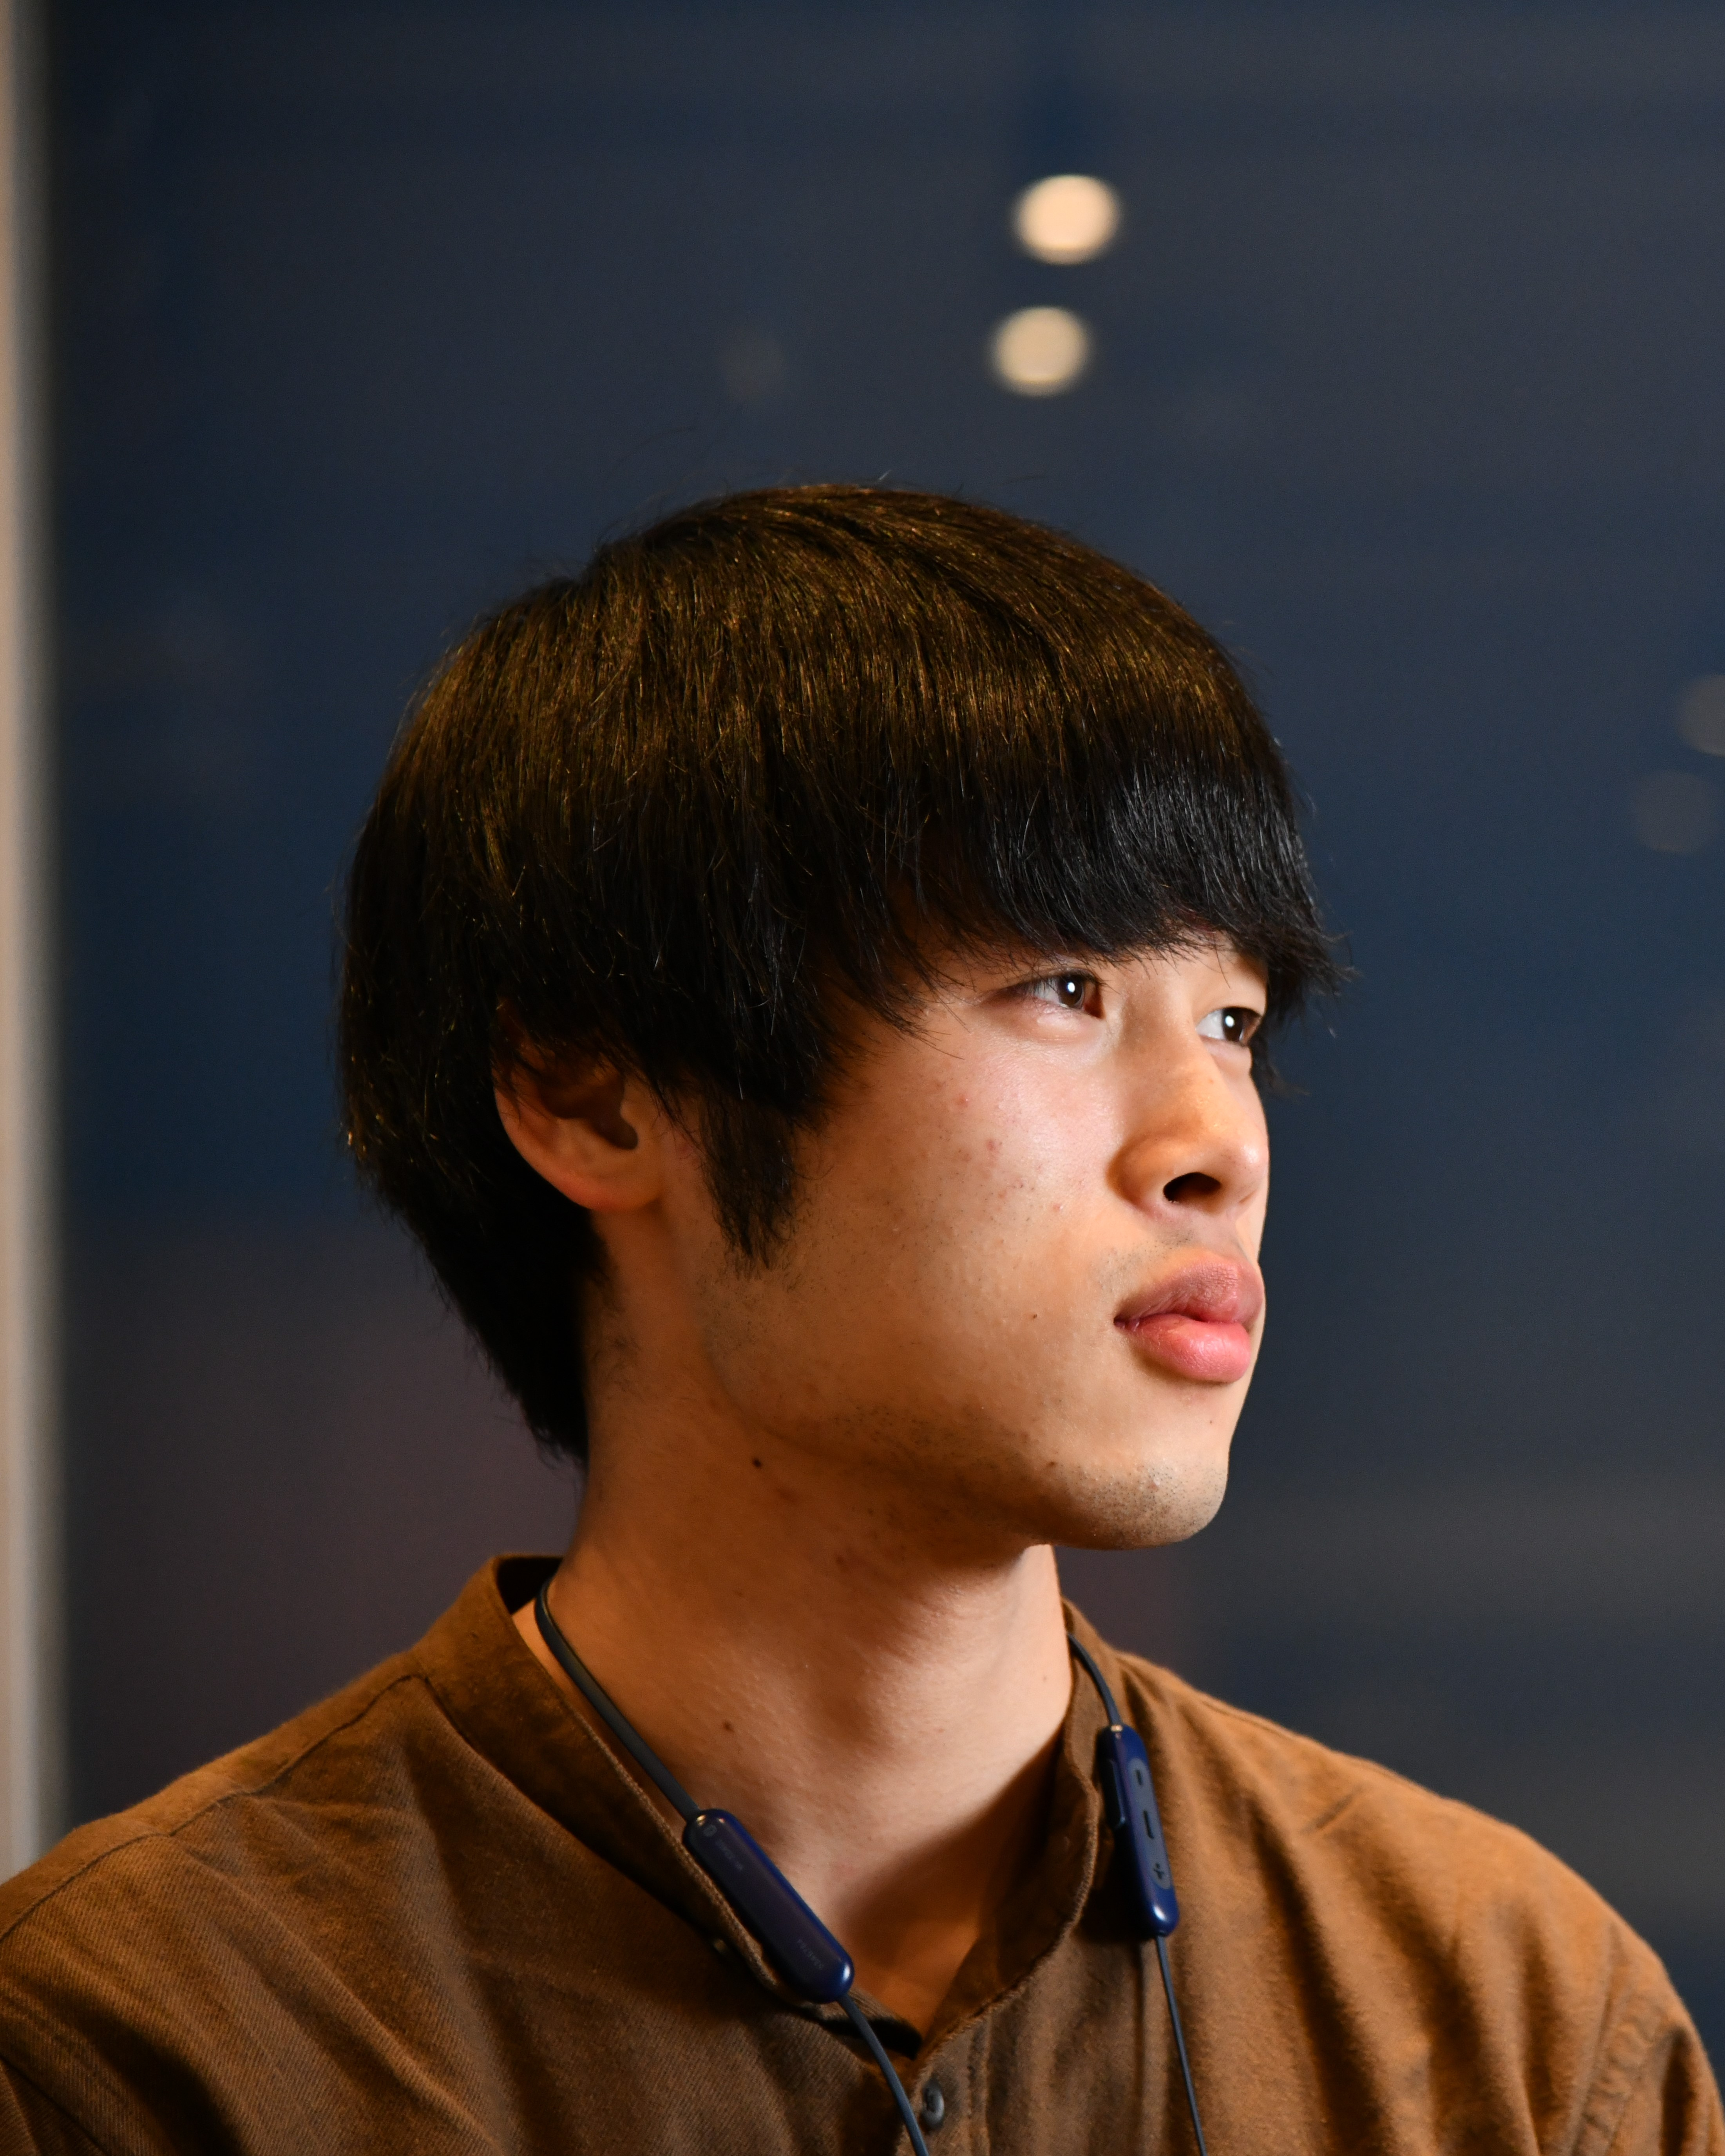
\includegraphics[width=1in,height=1.25in,clip,keepaspectratio]{./fig_supplement/ST_prof_4_5.JPG}}]{Shingo Takemoto}
    (S’22) received a B.E. degree and M.E. degree in Information and Computer Sciences in 2021 from Sophia University and in 2023 from Tokyo Institute of Technology, respectively. 
    
    He is currently pursuing an Ph.D. degree at the Department of Computer Science in the Tokyo Institute of Technology. 
    His current research interests are in signal and image processing and optimization theory.
    
    Mr. Takemoto received the Student Award from IEEE SPS Tokyo Joint Chapter in 2022.
\end{IEEEbiography}

\begin{IEEEbiography}[{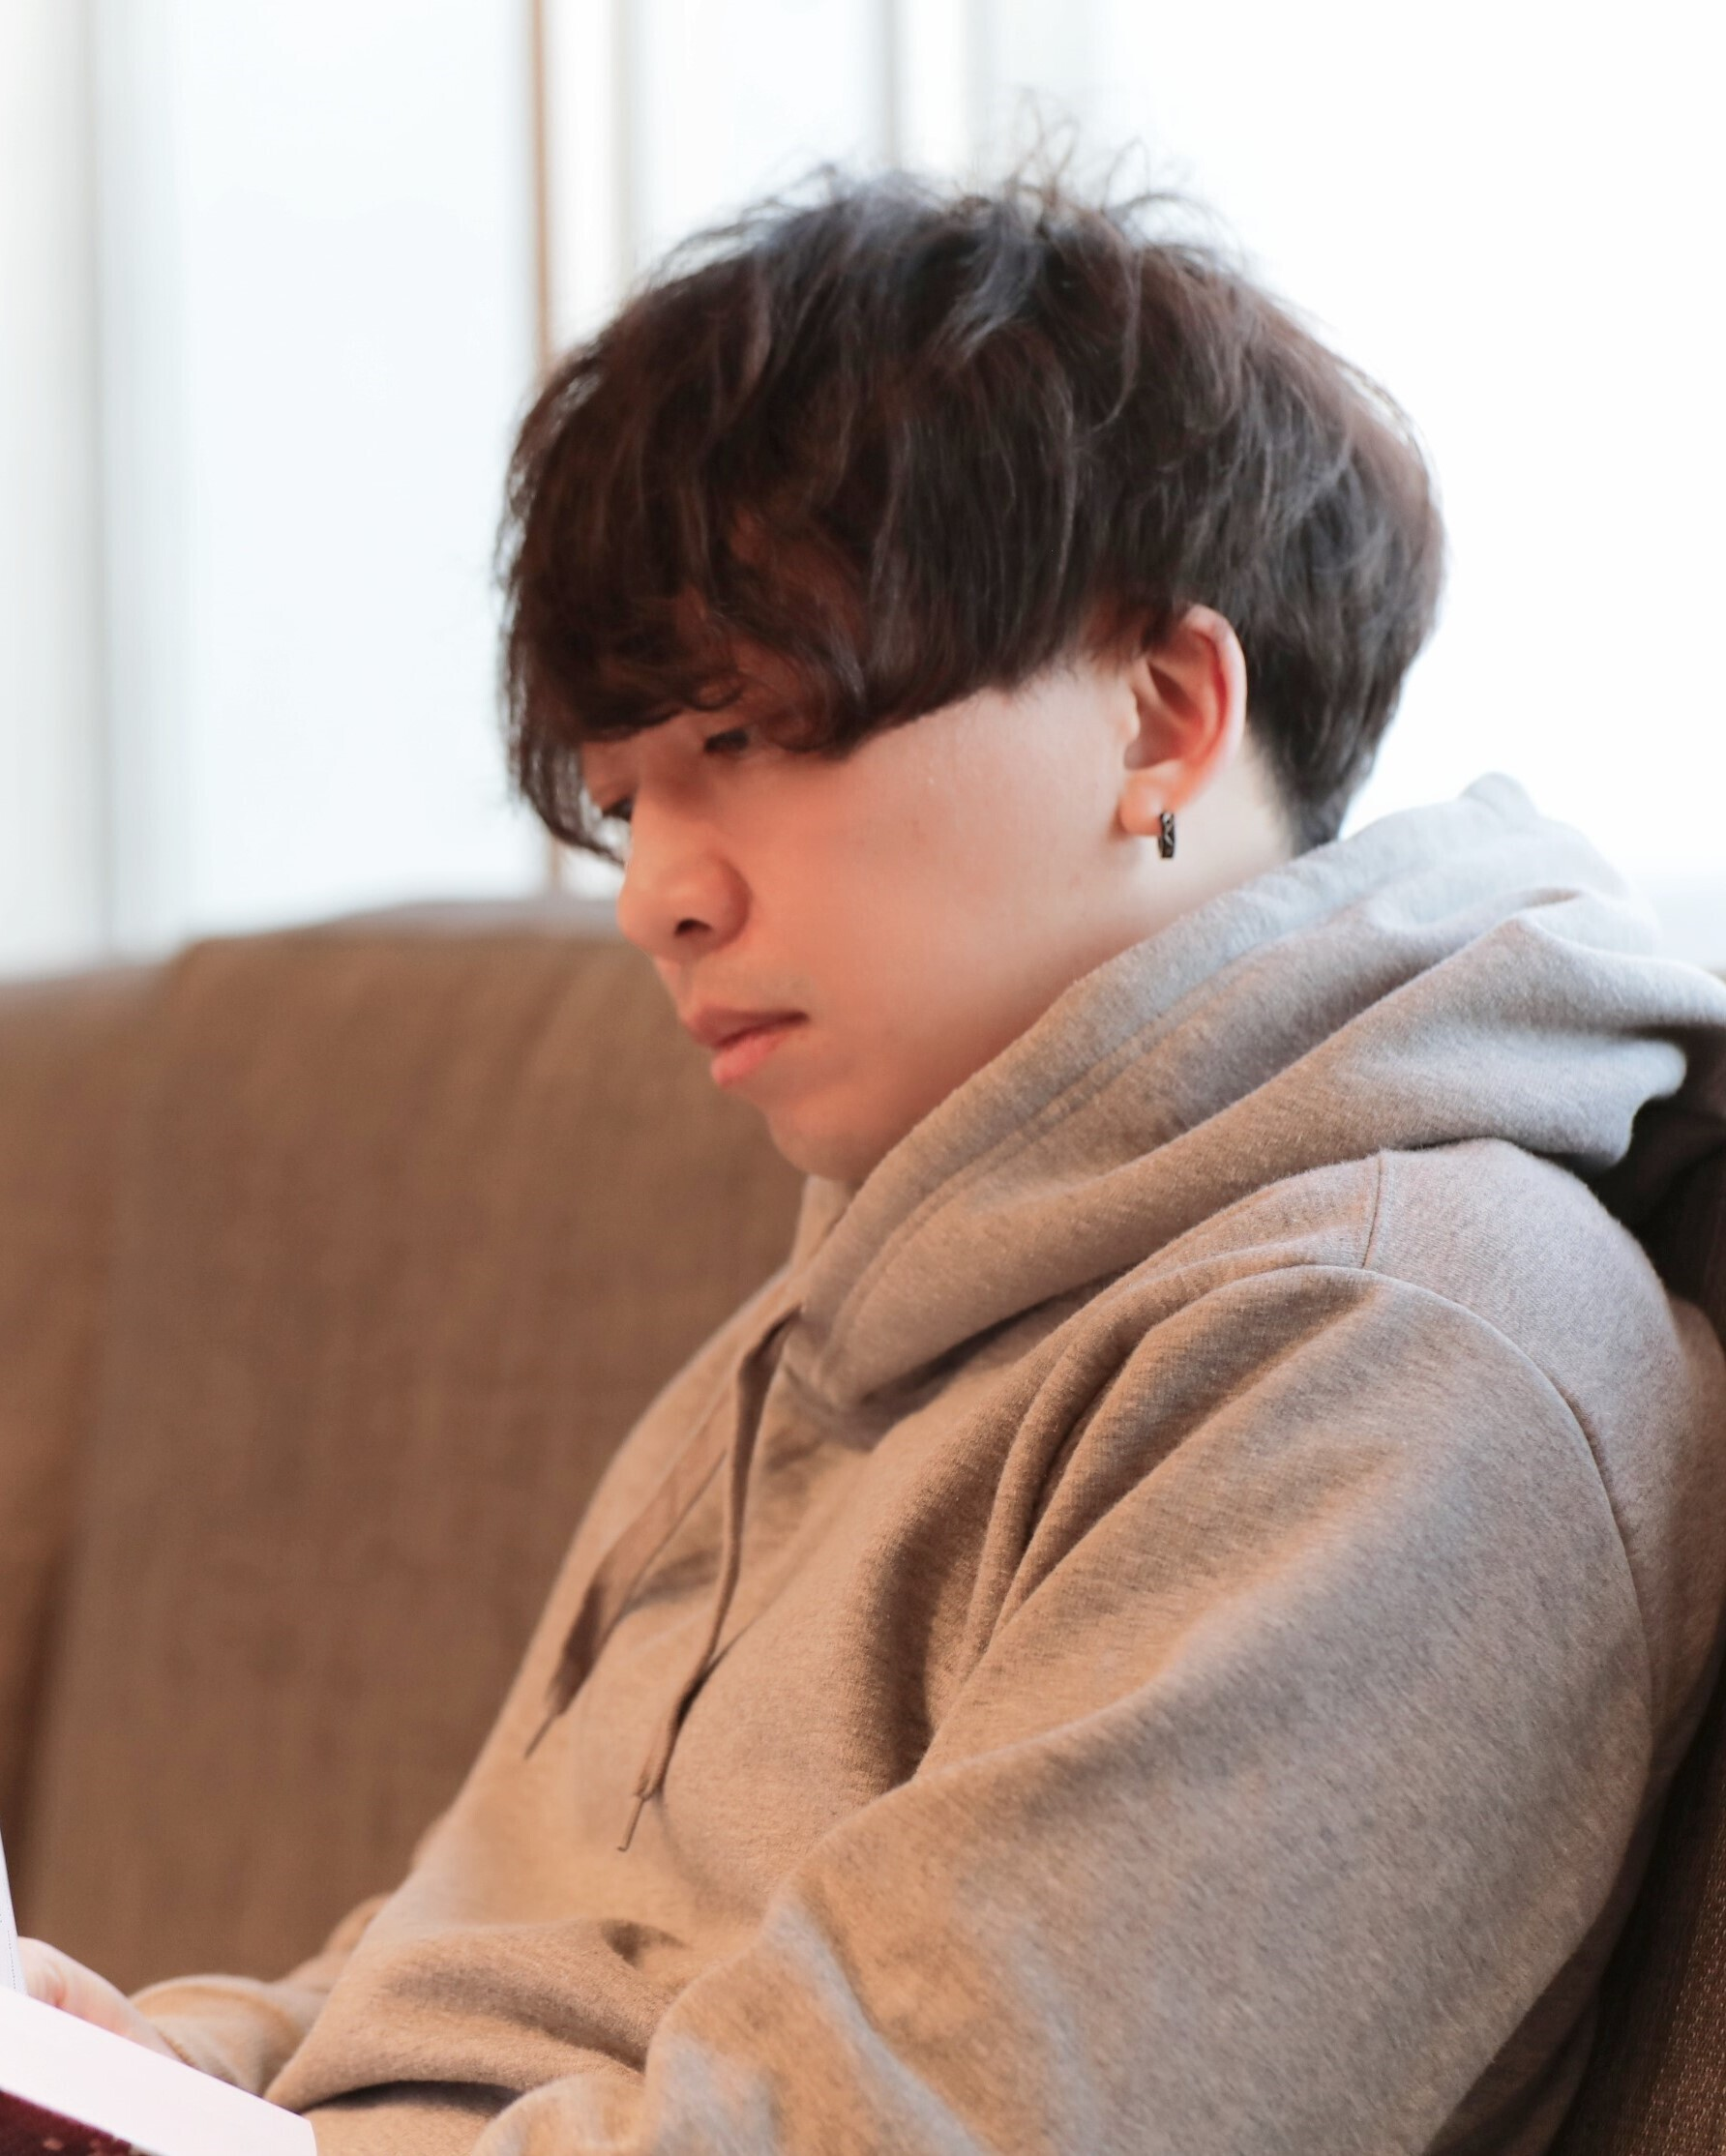
\includegraphics[width=1in,height=1.25in,clip,keepaspectratio]{./fig_supplement/prof_ono_book_bio.jpg}}]{Shunsuke Ono}
(S’11–M’15–SM'23) received a B.E. degree in Computer Science in 2010 and M.E. and Ph.D. degrees in Communications and Computer Engineering in 2012 and 2014 from the Tokyo Institute of Technology, respectively.

From April 2012 to September 2014, he was a Research Fellow (DC1) of the Japan Society for the Promotion of Science (JSPS). He is currently an Associate Professor in the Department of Computer Science, School of Computing, Tokyo Institute of Technology. From October 2016 to March 2020 and from October 2021 to present, he was/is a Researcher of Precursory Research for Embryonic Science and Technology (PRESTO), Japan Science and Technology Agency (JST), Tokyo, Japan. His research interests include signal processing, image analysis, remote sensing, mathematical optimization, and data science.

Dr. Ono received the Young Researchers’ Award and the Excellent Paper Award from the IEICE in 2013 and 2014, respectively, the Outstanding Student Journal Paper Award and the Young Author Best Paper Award from the IEEE SPS Japan Chapter in 2014 and 2020, respectively, the Funai Research Award from the Funai Foundation in 2017, the Ando Incentive Prize from the Foundation of Ando Laboratory in 2021, the Young Scientists’ Award from MEXT in 2022, and the Outstanding Editorial Board Member Award from IEEE SPS in 2023. He has been an Associate Editor of IEEE TRANSACTIONS ON SIGNAL AND INFORMATION PROCESSING OVER NETWORKS since 2019.
\end{IEEEbiography}




\vfill

\end{document}


